% Options for packages loaded elsewhere
\PassOptionsToPackage{unicode}{hyperref}
\PassOptionsToPackage{hyphens}{url}
%
\documentclass[
  11pt,
  letterpaper,
]{scrbook}

\usepackage{amsmath,amssymb}
\usepackage{iftex}
\ifPDFTeX
  \usepackage[T1]{fontenc}
  \usepackage[utf8]{inputenc}
  \usepackage{textcomp} % provide euro and other symbols
\else % if luatex or xetex
  \usepackage{unicode-math}
  \defaultfontfeatures{Scale=MatchLowercase}
  \defaultfontfeatures[\rmfamily]{Ligatures=TeX,Scale=1}
\fi
\usepackage{lmodern}
\ifPDFTeX\else  
    % xetex/luatex font selection
\fi
% Use upquote if available, for straight quotes in verbatim environments
\IfFileExists{upquote.sty}{\usepackage{upquote}}{}
\IfFileExists{microtype.sty}{% use microtype if available
  \usepackage[]{microtype}
  \UseMicrotypeSet[protrusion]{basicmath} % disable protrusion for tt fonts
}{}
\makeatletter
\@ifundefined{KOMAClassName}{% if non-KOMA class
  \IfFileExists{parskip.sty}{%
    \usepackage{parskip}
  }{% else
    \setlength{\parindent}{0pt}
    \setlength{\parskip}{6pt plus 2pt minus 1pt}}
}{% if KOMA class
  \KOMAoptions{parskip=half}}
\makeatother
\usepackage{xcolor}
\usepackage{svg}
\usepackage{soul}
\setlength{\emergencystretch}{3em} % prevent overfull lines
\setcounter{secnumdepth}{5}
% Make \paragraph and \subparagraph free-standing
\ifx\paragraph\undefined\else
  \let\oldparagraph\paragraph
  \renewcommand{\paragraph}[1]{\oldparagraph{#1}\mbox{}}
\fi
\ifx\subparagraph\undefined\else
  \let\oldsubparagraph\subparagraph
  \renewcommand{\subparagraph}[1]{\oldsubparagraph{#1}\mbox{}}
\fi

\usepackage{color}
\usepackage{fancyvrb}
\newcommand{\VerbBar}{|}
\newcommand{\VERB}{\Verb[commandchars=\\\{\}]}
\DefineVerbatimEnvironment{Highlighting}{Verbatim}{commandchars=\\\{\}}
% Add ',fontsize=\small' for more characters per line
\usepackage{framed}
\definecolor{shadecolor}{RGB}{241,243,245}
\newenvironment{Shaded}{\begin{snugshade}}{\end{snugshade}}
\newcommand{\AlertTok}[1]{\textcolor[rgb]{0.68,0.00,0.00}{#1}}
\newcommand{\AnnotationTok}[1]{\textcolor[rgb]{0.37,0.37,0.37}{#1}}
\newcommand{\AttributeTok}[1]{\textcolor[rgb]{0.40,0.45,0.13}{#1}}
\newcommand{\BaseNTok}[1]{\textcolor[rgb]{0.68,0.00,0.00}{#1}}
\newcommand{\BuiltInTok}[1]{\textcolor[rgb]{0.00,0.23,0.31}{#1}}
\newcommand{\CharTok}[1]{\textcolor[rgb]{0.13,0.47,0.30}{#1}}
\newcommand{\CommentTok}[1]{\textcolor[rgb]{0.37,0.37,0.37}{#1}}
\newcommand{\CommentVarTok}[1]{\textcolor[rgb]{0.37,0.37,0.37}{\textit{#1}}}
\newcommand{\ConstantTok}[1]{\textcolor[rgb]{0.56,0.35,0.01}{#1}}
\newcommand{\ControlFlowTok}[1]{\textcolor[rgb]{0.00,0.23,0.31}{#1}}
\newcommand{\DataTypeTok}[1]{\textcolor[rgb]{0.68,0.00,0.00}{#1}}
\newcommand{\DecValTok}[1]{\textcolor[rgb]{0.68,0.00,0.00}{#1}}
\newcommand{\DocumentationTok}[1]{\textcolor[rgb]{0.37,0.37,0.37}{\textit{#1}}}
\newcommand{\ErrorTok}[1]{\textcolor[rgb]{0.68,0.00,0.00}{#1}}
\newcommand{\ExtensionTok}[1]{\textcolor[rgb]{0.00,0.23,0.31}{#1}}
\newcommand{\FloatTok}[1]{\textcolor[rgb]{0.68,0.00,0.00}{#1}}
\newcommand{\FunctionTok}[1]{\textcolor[rgb]{0.28,0.35,0.67}{#1}}
\newcommand{\ImportTok}[1]{\textcolor[rgb]{0.00,0.46,0.62}{#1}}
\newcommand{\InformationTok}[1]{\textcolor[rgb]{0.37,0.37,0.37}{#1}}
\newcommand{\KeywordTok}[1]{\textcolor[rgb]{0.00,0.23,0.31}{#1}}
\newcommand{\NormalTok}[1]{\textcolor[rgb]{0.00,0.23,0.31}{#1}}
\newcommand{\OperatorTok}[1]{\textcolor[rgb]{0.37,0.37,0.37}{#1}}
\newcommand{\OtherTok}[1]{\textcolor[rgb]{0.00,0.23,0.31}{#1}}
\newcommand{\PreprocessorTok}[1]{\textcolor[rgb]{0.68,0.00,0.00}{#1}}
\newcommand{\RegionMarkerTok}[1]{\textcolor[rgb]{0.00,0.23,0.31}{#1}}
\newcommand{\SpecialCharTok}[1]{\textcolor[rgb]{0.37,0.37,0.37}{#1}}
\newcommand{\SpecialStringTok}[1]{\textcolor[rgb]{0.13,0.47,0.30}{#1}}
\newcommand{\StringTok}[1]{\textcolor[rgb]{0.13,0.47,0.30}{#1}}
\newcommand{\VariableTok}[1]{\textcolor[rgb]{0.07,0.07,0.07}{#1}}
\newcommand{\VerbatimStringTok}[1]{\textcolor[rgb]{0.13,0.47,0.30}{#1}}
\newcommand{\WarningTok}[1]{\textcolor[rgb]{0.37,0.37,0.37}{\textit{#1}}}

\providecommand{\tightlist}{%
  \setlength{\itemsep}{0pt}\setlength{\parskip}{0pt}}\usepackage{longtable,booktabs,array}
\usepackage{calc} % for calculating minipage widths
% Correct order of tables after \paragraph or \subparagraph
\usepackage{etoolbox}
\makeatletter
\patchcmd\longtable{\par}{\if@noskipsec\mbox{}\fi\par}{}{}
\makeatother
% Allow footnotes in longtable head/foot
\IfFileExists{footnotehyper.sty}{\usepackage{footnotehyper}}{\usepackage{footnote}}
\makesavenoteenv{longtable}
\usepackage{graphicx}
\makeatletter
\def\maxwidth{\ifdim\Gin@nat@width>\linewidth\linewidth\else\Gin@nat@width\fi}
\def\maxheight{\ifdim\Gin@nat@height>\textheight\textheight\else\Gin@nat@height\fi}
\makeatother
% Scale images if necessary, so that they will not overflow the page
% margins by default, and it is still possible to overwrite the defaults
% using explicit options in \includegraphics[width, height, ...]{}
\setkeys{Gin}{width=\maxwidth,height=\maxheight,keepaspectratio}
% Set default figure placement to htbp
\makeatletter
\def\fps@figure{htbp}
\makeatother
\newlength{\cslhangindent}
\setlength{\cslhangindent}{1.5em}
\newlength{\csllabelwidth}
\setlength{\csllabelwidth}{3em}
\newlength{\cslentryspacingunit} % times entry-spacing
\setlength{\cslentryspacingunit}{\parskip}
\newenvironment{CSLReferences}[2] % #1 hanging-ident, #2 entry spacing
 {% don't indent paragraphs
  \setlength{\parindent}{0pt}
  % turn on hanging indent if param 1 is 1
  \ifodd #1
  \let\oldpar\par
  \def\par{\hangindent=\cslhangindent\oldpar}
  \fi
  % set entry spacing
  \setlength{\parskip}{#2\cslentryspacingunit}
 }%
 {}
\usepackage{calc}
\newcommand{\CSLBlock}[1]{#1\hfill\break}
\newcommand{\CSLLeftMargin}[1]{\parbox[t]{\csllabelwidth}{#1}}
\newcommand{\CSLRightInline}[1]{\parbox[t]{\linewidth - \csllabelwidth}{#1}\break}
\newcommand{\CSLIndent}[1]{\hspace{\cslhangindent}#1}

\usepackage{booktabs}
\usepackage{caption}
\usepackage{longtable}
\makeatletter
\@ifpackageloaded{tcolorbox}{}{\usepackage[skins,breakable]{tcolorbox}}
\@ifpackageloaded{fontawesome5}{}{\usepackage{fontawesome5}}
\definecolor{quarto-callout-color}{HTML}{909090}
\definecolor{quarto-callout-note-color}{HTML}{0758E5}
\definecolor{quarto-callout-important-color}{HTML}{CC1914}
\definecolor{quarto-callout-warning-color}{HTML}{EB9113}
\definecolor{quarto-callout-tip-color}{HTML}{00A047}
\definecolor{quarto-callout-caution-color}{HTML}{FC5300}
\definecolor{quarto-callout-color-frame}{HTML}{acacac}
\definecolor{quarto-callout-note-color-frame}{HTML}{4582ec}
\definecolor{quarto-callout-important-color-frame}{HTML}{d9534f}
\definecolor{quarto-callout-warning-color-frame}{HTML}{f0ad4e}
\definecolor{quarto-callout-tip-color-frame}{HTML}{02b875}
\definecolor{quarto-callout-caution-color-frame}{HTML}{fd7e14}
\makeatother
\makeatletter
\makeatother
\makeatletter
\@ifpackageloaded{bookmark}{}{\usepackage{bookmark}}
\makeatother
\makeatletter
\@ifpackageloaded{caption}{}{\usepackage{caption}}
\AtBeginDocument{%
\ifdefined\contentsname
  \renewcommand*\contentsname{Table of contents}
\else
  \newcommand\contentsname{Table of contents}
\fi
\ifdefined\listfigurename
  \renewcommand*\listfigurename{List of Figures}
\else
  \newcommand\listfigurename{List of Figures}
\fi
\ifdefined\listtablename
  \renewcommand*\listtablename{List of Tables}
\else
  \newcommand\listtablename{List of Tables}
\fi
\ifdefined\figurename
  \renewcommand*\figurename{Figure}
\else
  \newcommand\figurename{Figure}
\fi
\ifdefined\tablename
  \renewcommand*\tablename{Table}
\else
  \newcommand\tablename{Table}
\fi
}
\@ifpackageloaded{float}{}{\usepackage{float}}
\floatstyle{ruled}
\@ifundefined{c@chapter}{\newfloat{codelisting}{h}{lop}}{\newfloat{codelisting}{h}{lop}[chapter]}
\floatname{codelisting}{Listing}
\newcommand*\listoflistings{\listof{codelisting}{List of Listings}}
\makeatother
\makeatletter
\@ifpackageloaded{caption}{}{\usepackage{caption}}
\@ifpackageloaded{subcaption}{}{\usepackage{subcaption}}
\makeatother
\makeatletter
\@ifpackageloaded{tcolorbox}{}{\usepackage[skins,breakable]{tcolorbox}}
\makeatother
\makeatletter
\@ifundefined{shadecolor}{\definecolor{shadecolor}{rgb}{.97, .97, .97}}
\makeatother
\makeatletter
\makeatother
\makeatletter
\makeatother
\ifLuaTeX
  \usepackage{selnolig}  % disable illegal ligatures
\fi
\IfFileExists{bookmark.sty}{\usepackage{bookmark}}{\usepackage{hyperref}}
\IfFileExists{xurl.sty}{\usepackage{xurl}}{} % add URL line breaks if available
\urlstyle{same} % disable monospaced font for URLs
\hypersetup{
  pdftitle={Quantitative methods and statistics (In Sport and Exercise Science)},
  pdfauthor={Daniel Hammarström},
  hidelinks,
  pdfcreator={LaTeX via pandoc}}

\title{Quantitative methods and statistics (In Sport and Exercise
Science)}
\author{Daniel Hammarström}
\date{2023-07-31}

\begin{document}
\frontmatter
\maketitle
\ifdefined\Shaded\renewenvironment{Shaded}{\begin{tcolorbox}[interior hidden, borderline west={3pt}{0pt}{shadecolor}, enhanced, breakable, frame hidden, sharp corners, boxrule=0pt]}{\end{tcolorbox}}\fi

\renewcommand*\contentsname{Table of contents}
{
\setcounter{tocdepth}{2}
\tableofcontents
}
\mainmatter
\bookmarksetup{startatroot}

\hypertarget{quantitative-methods-and-statistics-in-sport-and-exercise-science}{%
\chapter{Quantitative methods and statistics (In Sport and Exercise
Science)}\label{quantitative-methods-and-statistics-in-sport-and-exercise-science}}

\bookmarksetup{startatroot}

\hypertarget{introduction}{%
\chapter{Introduction}\label{introduction}}

Welcome to the course \textbf{Quantitative methods and Statistics
(IDR4000)}. The course aims to give students an overview of
methodological aspects within the field of sport and
exercise-physiology. Specifically, planning, conducting and analyzing
research projects with human participants will be covered. These course
notes covers \emph{almost} the entire course through the combination of
video lectures, tutorials and references to the course literature and
external resources.

This book contains lecture notes for the course. Assignments, tutorials
and other cours material has been moved to the
\href{https://dhammarstrom.github.io/quant-methods-workshops/}{course
workshop site}

\hypertarget{prerequisites}{%
\section{Prerequisites}\label{prerequisites}}

\bookmarksetup{startatroot}

\hypertarget{introduction-to-data-science}{%
\chapter{Introduction to data
science}\label{introduction-to-data-science}}

\hypertarget{about-data-in-the-world-of-sport-and-exercise}{%
\section{About data in the world of sport and
exercise}\label{about-data-in-the-world-of-sport-and-exercise}}

Data are everywhere. Most of us always walk around with a data
collection device in our pockets. This device (your mobile phone)
records and store data about you throughout the day. Such data are the
basis of the \emph{quantified self-movement}\footnote{Cheat sheets are
  available in R Studio: \emph{Help \textgreater{} Cheatsheets}}, which
has grown in popularity as capabilities to record data from daily life
have improved. People interested in quantifying their personal life does
so for different reasons, but often with the intent to improve their
health\footnote{See this website for
  \href{https://quantifiedself.com/show-and-tell/}{intriguing examples}}.

Much of this kind of data is readily available to us because data
privacy policies regard it as personal \footnote{See
  e.g.~\href{https://www.apple.com/legal/privacy/en-ww/}{Apples Privacy
  Policy}.}. With some effort, you can get your data out of your iPhone
to explore, for example, your daily step count. I discovered that my
phone(s) has been collecting data for me since 2016, and I tend to walk
fewer steps on Sundays than Saturdays (see Figure
Figure~\ref{fig-iphone}).

\begin{figure}

{\centering 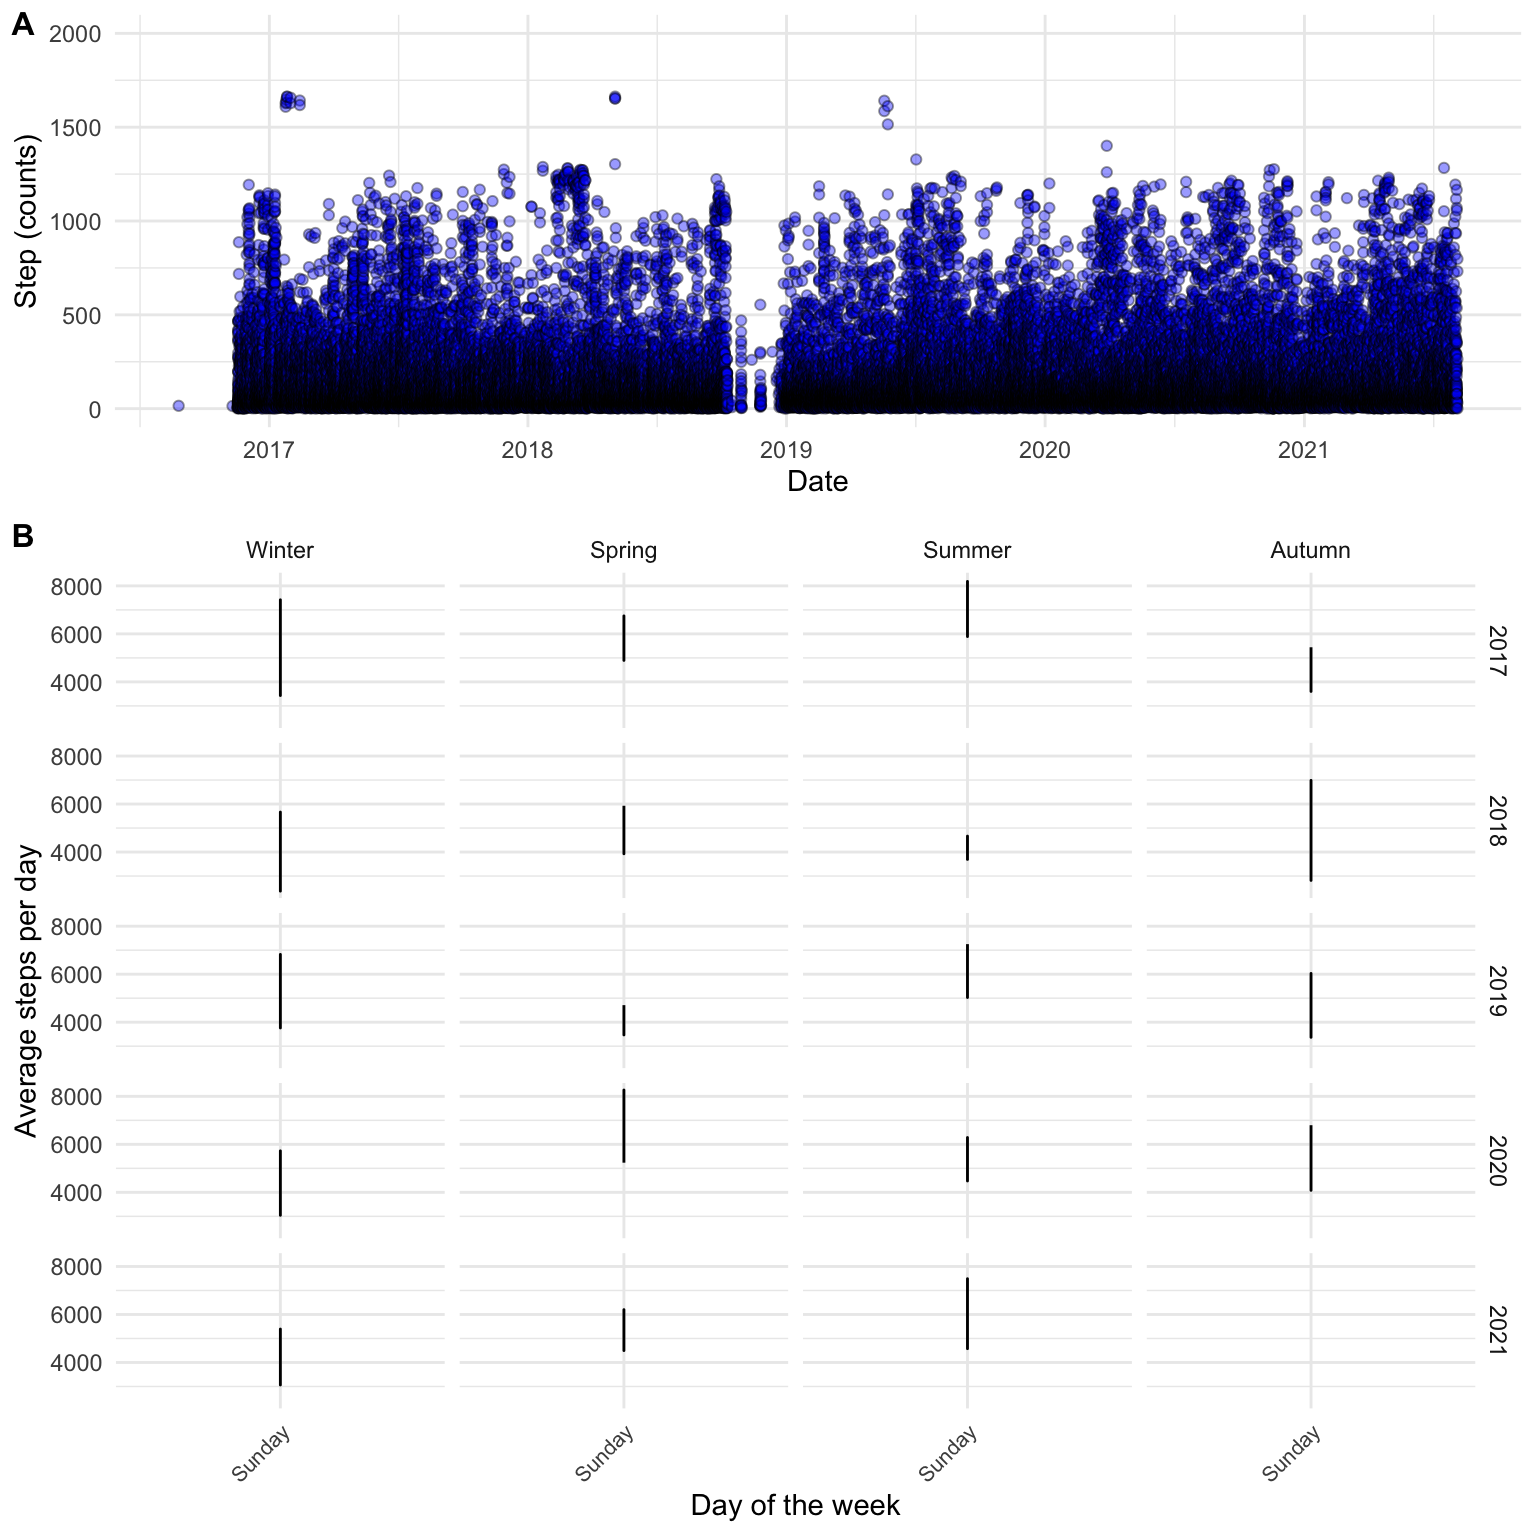
\includegraphics{01-intro-to-data_files/figure-pdf/fig-iphone-1.pdf}

}

\caption{\label{fig-iphone}Step count data from my iPhone displayed as
all avalable data points (A, after data cleaning) and average step per
weekday, per year and season (B).}

\end{figure}

Data are also collected and stored in publicly available databases. Such
databases are created for the purpose of storing specific types of data,
such as soccer\footnote{\href{https://understat.com/}{understat.com}
  stores match specific data from major leagues. Data are available
  through software packages such as
  \href{https://jaseziv.github.io/worldfootballR/index.html}{\texttt{worldfootballR}}}
or biathlon results\footnote{\href{https://biathlonresults.com/}{biathlonresults.com/}
  hosts results from the international biathlon federation. An example
  of analyzed data can be
  \href{https://sciathlon.github.io/post/biathlon_data_analysis/}{seen
  here}.}, or biological information, such as gene sequences\footnote{\href{https://www.ensembl.org/}{Ensembl}
  and the \href{https://www.ncbi.nlm.nih.gov/}{National center for
  biotechnology information} are commonly used databases in the
  biomedical sciences.}. Even data from scientific studies are often
publicly available\footnote{We published our raw data together with a
  recent paper (Mølmen et al 2021
  \href{https://translational-medicine.biomedcentral.com/articles/10.1186/s12967-021-02969-1}{doi:
  10.1186/s12967-021-02969-1.}) together with code to analyze it in a
  \href{https://github.com/dhammarstrom/rnaseq-copd}{public repository}.},
meaning we can perform scientific studies on unique data sets without
collecting the data ourselves.

The above examples show an abundance of available data. The problem is
that to understand a phenomenon better, we need techniques and methods
to make sense of the data, and this is where data science and data
literacy comes in. In the world of sports and exercise, regardless if
you are interested in doing scientific investigations, coaching a soccer
team or individual athletes, or helping patients recover from surgery
using exercise therapy, you are faced with the problem of handling and
making sense of data. Essential skills and a deeper understanding of
data science are transferable between such areas of practice. One
broader aim of this course is for you to develop skills to better
understand data.

\begin{quote}
\textbf{Think about the literature!} Spiegelhalter (The Art of
Statistics, in the introduction chapter) talks about how statistics has
evolved towards the broader field of data science. In data science,
statistical theory and methods are just parts of the problem solving
cycle. Try to think about how you would use the PPDAC cycle as a
exercise coach and a scientist. What are the similarities and
differences?
\end{quote}

\hypertarget{replication-and-reproducibility}{%
\section{Replication and
Reproducibility}\label{replication-and-reproducibility}}

In scientific research, replication is a way to confirm scientific
claims. When an independent group of researchers can confirm a result,
the claim is more likely to be true. However, many results will be
impossible to replicate due to the size of trials, costs, and urgency of
the research question. A recent example is the many vaccine trials
performed to develop a vaccine against COVID-19\footnote{https://www.evaluate.com/vantage/articles/news/snippets/its-official-covid-19-vaccine-trials-rank-among-largest}.
Other examples concern studies with unique study populations, such as
large-scale epidemiological studies (Peng, Dominici, and Zeger 2006),
but the same is true for unique investigations in sport and exercise
science.

When studies are not likely to be \emph{replicated},
\emph{reproducibility} of the analyses and results has been suggested to
be a minimum standard for scientific studies. Reproducibility means that
independent researchers can draw similar results or conclusions from the
same data (Peng, Dominici, and Zeger 2006).

Peng et al. (Peng, Dominici, and Zeger 2006) suggests that a \emph{fully
reproducible} study has

\begin{itemize}
\tightlist
\item
  Available data.
\item
  Computer code (software) that produces the results of the study.
\item
  Documentation that describes the software and data used in the study,
  and
\item
  ways to share the data and code.
\end{itemize}

The above principally relates to the trust we can place in scientific
results. However, the minimum reproducibility standard also has
advantages for the individual researcher (or master's student)! When
working with reproducible methods, we will develop ways of documenting
and automating our analyses. This way of working with analyses will make
it easier to collaborate with others. And, as it turns out, your most
frequent collaborator is you in the future!

Reproducible data analysis means that you will make it explicit and
transparent. In traditional data analysis, most activities are in the
``black box.'' To avoid bias (Ioannidis 2005), the ``black box'' needs
to be opened, and you need to actively make transparent decisions all
along the analytic pipeline (Leek and Peng 2015). This pipeline
preferably involves the whole problem-solving cycle described by
Spiegelhalter (Spiegelhalter 2019). However, the tools we will learn in
this course focus primarily on the steps from the experimental design to
the presentation of statistical results (Leek and Peng 2015). These
steps include data collection (and storage), data cleaning, exploratory
data analysis, statistical modeling, and statistical inference (and
communication) (Leek and Peng 2015).

\hypertarget{tools-in-data-science}{%
\section{Tools in data science}\label{tools-in-data-science}}

Ways to interpret and make sense of data involve different methods.
These methods are often implemented in computer software, which means
that when you want to understand data as a practitioner (scientist,
coach, analyst), you must master some computer software. Microsoft's
Excel is one of the most common software used to understand data, even
among professional data scientists\footnote{(See for example this
  ranking){[}https://www.kdnuggets.com/2019/05/poll-top-data-science-machine-learning-platforms.html{]}.}.
You can do fantastic stuff with Excel! In the world of sport and
exercise, Excel has been used in diverse activities such as scientific
investigations, planning and recording training for world
champions\footnote{The amount of time used by different coaches to
  create their own specific coaching software really makes many of them
  amateur software engineers. See for example this training journal from
  \href{http://obasen.orientering.se/traningsdagbok/installationshandledning.htm}{swedish
  orienteering}.}, and scheduling appointments.

For scientific research, most people use additional software to do
statistical analyses. If you have spent time in higher education, you
have probably heard about SPSS, Stata, or Jamovi. These are all
specialized software used for statistical analyses.

The tools mentioned above can all be used as part of a fully
reproducible workflow. However, some software solutions suit this
requirement better than others. Going back to the description of
reproducible science as made by Peng et al. (Peng, Dominici, and Zeger
2006), we want software where analyses can be

\begin{itemize}
\tightlist
\item
  Human- and computer-readable, meaning that we want to be able to write
  scripts or computer programs that execute the analyses.
\item
  Documented, meaning that along the code, we want to be able to
  describe what the code does.
\item
  Available and able to share with others, meaning that our analyses can
  be run on open and free software to maximize the ability to share
  them.
\end{itemize}

This means that the software we would prefer should be run using scripts
(as opposed to point and click) and be free of charge (and open source,
as opposed to expensive and proprietary). These criteria can be
fulfilled when we use software written around the R language (although
alternatives exist \footnote{In addition to R, Python offers a free open
  source environment for reproducible analyses. The choice between the
  two are
  \href{https://www.datacamp.com/community/tutorials/r-or-python-for-data-analysis}{matter
  of taste}.}).

R is a computer language especially well suited for reproducible data
analysis. As users can contribute software extensions, also called
packages, many specialized software implementations exist for tasks such
as creating figures or analyzing specific data. Around R, people have
been developing auxiliary software for reproducible data analysis. The
negative part of all these opportunities is that using R requires
effort. The learning curve is steep!

Even though you might not use R ever again after this course, trying to
learn it will let you know something about programming, modern data
science capabilities, statistical analysis, and software/computers in
general. These areas are all aspects of our modern society and are
transferable regardless of what computer language we are talking about.

A big challenge when working with complex analyses or other large
projects over time is keeping track of changes. Another challenge might
be effective collaboration with others and with yourself in the future.
To overcome these challenges, we can use a version control system
connected to a social platform for distributing computer code and data.
Github is a web-based platform that provides this functionality. It is a
potent combination if you want to collaborate and share what you are
working on.

\hypertarget{installing-and-getting-to-know-the-required-software}{%
\section{Installing and getting to know the required
software}\label{installing-and-getting-to-know-the-required-software}}

As noted above, there are multiple computer languages and software
solutions that could satisfy our needs. However, in this course, we will
focus on a combination of continuously improved tools to make it easy
for the user to collaborate and communicate data analyses. Below is a
checklist of what you must install on your system to take full advantage
of the proposed tools.

\hypertarget{r-and-rstudio}{%
\subsection{R and RStudio}\label{r-and-rstudio}}

\textbf{R} is a free,
\href{https://en.wikipedia.org/wiki/Open_source}{open-source} software
designed for statistical computing. We will use R as a part of an
environment (using R Studio, introduced below). To download and install
R:

\begin{enumerate}
\def\labelenumi{\arabic{enumi}.}
\item
  Go to \url{https://cran.uib.no/},
\item
  Select your operating system (Download R for Windows, MacOS or Linux).

  \begin{itemize}
  \tightlist
  \item
    If you have Windows, choose \texttt{base}, click on ``Download R
    (\ldots) for windows'', save and run the file. The installation
    process should be self explanatory.
  \item
    If you have MacOS, download and install the latest release.
  \end{itemize}
\item
  Run the installer to install R.
\end{enumerate}

\textbf{\href{https://www.posit.co/}{RStudio}} is a software designed to
make it easier to use R. It is free to download and use. It is designed
as an \textbf{integrated development environment} that lets you organize
your work together with R and other tools. Install it by going to
\url{https://www.posit.co/}.

\begin{enumerate}
\def\labelenumi{\arabic{enumi}.}
\tightlist
\item
  Select ``Products'' and \textbf{RStudio IDE}
\item
  Scroll down and find the \href{https://posit.co/downloads/}{FREE open
  source edition}
\item
  Download the installer made for your operating system.
\end{enumerate}

\hypertarget{git-and-github}{%
\subsection{Git and Github}\label{git-and-github}}

Git is a software that you need to install on your system in order to
use version control. Github is the web platform that allows
collaboration and web-based storage of your work. First, we will install
git.

For windows:

\begin{enumerate}
\def\labelenumi{\arabic{enumi}.}
\item
  If you have Windows, Go to \url{https://git-scm.com/downloads} and
  download the latest version for your operating system.
\item
  Run the installer. Make a note of where you installed it!
\end{enumerate}

For Mac:

\begin{enumerate}
\def\labelenumi{\arabic{enumi}.}
\item
  If you are on Mac, the easiest thing is to first install
  \href{https://brew.sh/}{\emph{Homebrew}}, this will make it easy to
  get the latest version of what we will need. Go to
  \url{https://brew.sh/} and follow the instructions. Note that you will
  need to open the terminal and enter the install command.
\item
  Install git by entering the follwing command in a freshly opened
  terminal:
\end{enumerate}

\texttt{brew\ install\ git}

Check if git was installed by restarting the terminal and write

\texttt{git\ -\/-version}

Additional warnings might appear indicating that you'll need some extra
software. More specifically, you might need Xcode command line tools. To
install these, go to your terminal and enter

\texttt{xcode-select\ -\/-install}

If you had problems with the homebrew installation itself or the brew
installation of git before, try again after installing xcode command
line tools.

\hypertarget{connecting-to-github}{%
\subsection{Connecting to GitHub}\label{connecting-to-github}}

First we will let RStudio know where git is located

\begin{enumerate}
\def\labelenumi{\arabic{enumi}.}
\tightlist
\item
  Open RStudio, go to \emph{Global Options} under the \emph{Tools} menu.
  Go to the \emph{Git/SVN} sub-menu and find the \textbf{folder where
  git.exe} is located by browsing in the \emph{``Git executable''}
  field.
\end{enumerate}

\textbf{On windows:}

If you have installed git using default settings your \texttt{git.exe}
should be located in \texttt{C:/Program\ Files/Git/bin/git.exe}.

\textbf{On Mac}:

If you have installed git using homebrew, your git version \emph{may} be
found in \texttt{/usr/local/bin/git}.

To register for a Github account

\begin{enumerate}
\def\labelenumi{\arabic{enumi}.}
\tightlist
\item
  Go to \href{www.github.com}{Github.com}.
\item
  Find ``Sign up'' and follow the instructions.
\end{enumerate}

Next we need to connect our git software to github. This is done by
\emph{authentication}.
\href{https://docs.github.com/en/authentication/keeping-your-account-and-data-secure/about-authentication-to-github}{There
are several options}, however below are two options that should work
right away!

\hypertarget{installing-github-desktop}{%
\subsubsection{Installing GitHub
desktop}\label{installing-github-desktop}}

\begin{enumerate}
\def\labelenumi{\arabic{enumi}.}
\tightlist
\item
  Go to \href{https://desktop.github.com/}{desktop.github.com}
\item
  Download the installer and follow the instructions.
\item
  Open GitHub Desktop and go to File \textgreater{} Options
  \textgreater{} Accounts and select \textbf{Sign In} to Github.com,
  follow the instructions
\end{enumerate}

\hypertarget{installing-github-cli}{%
\subsubsection{Installing Github CLI}\label{installing-github-cli}}

If you were successful in authenticating with Github desktop as
described above, you should be all set. However, as an alternative you
could install and use Github CLI. This is a collection of command line
commands that makes it easy to use github from the command line. I
recommend installing them:

\begin{enumerate}
\def\labelenumi{\arabic{enumi}.}
\tightlist
\item
  Go to \url{https://cli.github.com/} and follow the instructions.
\end{enumerate}

\begin{itemize}
\tightlist
\item
  For windows, install GitHub CLI with the installer.
\item
  For Mac, use homebrew: \texttt{brew\ install\ gh}
\end{itemize}

Next we will perform the authentication process:

\begin{enumerate}
\def\labelenumi{\arabic{enumi}.}
\tightlist
\item
  Open a terminal and type \texttt{gh\ auth\ login}, follow the
  instructions.
\end{enumerate}

Done!

\hypertarget{a-note-on-git-and-clients}{%
\subsection{A note on Git and clients}\label{a-note-on-git-and-clients}}

As noted above, git is a software containing a number of functions for
version control of files collected in a folder (or repository). A client
in this context refers to a \emph{user interface} that makes it easy to
communicate with git. RStudio has some features that makes it possible
to execute git commands by clicking, however this \emph{client} is not
very powerful, you might want another, or several other alternatives.

First, git is available from the command line. It might look like this:

\texttt{git\ add\ -A}

We will touch upon more git commands for the command line later. The
above adds all changes you have made to a list of changes that will be
included in your next snapshot of your project. More on that later!

Several Git clients can be run at the same time. This means that you
might do some git on the command line in a terminal window in RStudio,
and you might follow the changes in a graphical user interface, such as
\href{https://desktop.github.com/}{GitHub Desktop}. The graphical user
interface lets you navigate more easily and might help you understand
what git is doing. We will be using GitHub desktop, so you make sure you
have installed it (see above).

\hypertarget{quarto-and-friends}{%
\subsection{Quarto and friends}\label{quarto-and-friends}}

The R community has pioneered literate programming for data analysis by
early adoption of file formats that lets the user combine computer code
and output with text (Peng, Dominici, and Zeger 2006). A well adopted
file format in recent years have been
\href{https://rmarkdown.rstudio.com/}{R markdown} which combines R code
with text and lets the user compile reports in multiple output formats
from a source document. R markdown is an ``R-centric'' approach to
literate programming. Even though it lets you combine multiple computer
languages, all code execution goes through R. Recently, a new format has
been introduced, \href{https://quarto.org/}{Quarto}, which is not
executed through R but its own dedicated software, Quarto.

Rmarkdown and Quarto have many similarities in that you can use
markdown, a well established
\href{https://en.wikipedia.org/wiki/Markdown}{markup language} to format
text with a plain text editor (like notepad). This means that for the R
user, most differences between RMarkdown and quarto in formatting your
documents are irrelevant for getting started.

As quarto authoring requires its own software, we need to do some
installation.

\begin{enumerate}
\def\labelenumi{\arabic{enumi}.}
\tightlist
\item
  Go to \href{https://quarto.org/}{quarto.org}
\item
  Click ``\emph{Get Started}'' and follow the instructions.
\end{enumerate}

A nice output from a quarto source documents is a PDF. In order to
create PDFs using R/RStudio/quarto we need to install a version of the
typesetting system \href{https://en.wikipedia.org/wiki/TeX}{TeX}. Quarto
recommends\footnote{See the quarto documentation for details on creating
  pdfs and installing TeX distributions
  https://quarto.org/docs/output-formats/pdf-basics.html} using
\href{https://yihui.org/tinytex/}{tinytex} which is easily installed
after you have installed quarto.

\begin{enumerate}
\def\labelenumi{\arabic{enumi}.}
\tightlist
\item
  Open up RStudio and a fresh terminal
\item
  type \texttt{quarto\ install\ tinytex} and follow the instructions.
\end{enumerate}

You should be ready to go now!

\hypertarget{summing-up-and-where-to-find-help}{%
\section{Summing up and where to find
help}\label{summing-up-and-where-to-find-help}}

We have installed R, RStudio, git, GitHub desktop/CLI, quarto and
tinytex. You have also created a github account. These are the tools
that you will need to go further in this course. But what if you run
into problems? Do not worry, the internet is at your service! A lot of
people work very hard to make it easy for beginners to adopt their
tools. Documentation of the tools we have installed so far is available
through google or any other search engine. People are also very helpful
in answering questions, answers to large and small problems can be found
in forums such as \href{https://stackoverflow.com/}{stack overflow}(see
below).

Learning new skills, like doing data analysis by programming, can be
hard but rewarding. If you want to make your learning experience less
hard, consider these points:

\begin{itemize}
\tightlist
\item
  \textbf{There are (almost always) multiple solutions to a problem}.
  When faced with difficulties, do not give up trying to search for a
  perfect single solution. Instead know that there are multiple ways of
  defining the problem and therefore multiple ways of making stuff work.
\item
  \textbf{Someone else has already had the same problem}. The internet
  is full of questions and answers, also related to what ever problem
  you might have. Learning how to write ``googleable'' questions is a
  great skill. By adding ``in R'' to your problem in a google search
  term often helps finding R related solutions.
\item
  \textbf{Find your motivation}. The skills that you will learn in this
  course are transferable to countless potential work related roles for
  the future you! To be able to showcase these skills may lead you to
  your dream job! Find your motivation for learning how to analyze data
  and communicating insights!
\item
  \textbf{``Microdosing'' statistical learning}. Replace your social
  media influencers with R users and data scientists! I find R people on
  \href{twitter.com}{Twitter} and
  \href{https://joinmastodon.org/}{mastodon}. Tweets and posts in this
  format keeps your R brain going!
\end{itemize}

\hypertarget{a-small-list-of-reference-material-and-resources}{%
\subsection{A (small) list of reference material and
resources}\label{a-small-list-of-reference-material-and-resources}}

\begin{itemize}
\item
  \href{https://r4ds.hadley.nz/}{R for Data Science} is a very
  comprehensive guide to working with R. It can be used chapter by
  chapter or by looking for tips on specific subjects.
\item
  The official
  \href{https://cran.r-project.org/doc/manuals/R-intro.pdf}{An
  Introduction to R} released by the R Core Team gives a thorough
  overview of R. This document can be used to find explanations to basic
  R code.
\item
  \href{https://learningstatisticswithr.com/}{Learning statistics with
  R} Is a free textbook where statistical concepts are integrated with
  learning R. Use this book as a reference.
\item
  \href{https://happygitwithr.com/index.html}{Happy Git and GitHub for
  the useR} is used as background material for our workshop in version
  control and collaborative data analysis.
\item
  \href{https://www.tidyverse.org/}{Tidyverse} Is a collection of R
  packages that makes it easier to be productive in R. Here you will
  find documentation for ggplot, dplyr and tidyr which are all packages
  that we will use extensively in the course.
\item
  \href{https://stackoverflow.com/}{Stack overflow} is a web platform
  where users provide answers to questions raised by other users. Here
  you will find answers to many of your R-related questions. Stack
  overflow will likely come up if you google a R problem by you can also
  search the website.
\item
  \href{https://www.r-bloggers.com/}{R bloggers} collects blog posts
  from R users, here you can find interesting use cases of R and tips.
\end{itemize}

\hypertarget{references-and-footnotes}{%
\section{References and footnotes}\label{references-and-footnotes}}

\bookmarksetup{startatroot}

\hypertarget{storing-data-in-spreadsheets-and-understanding-tabular-data}{%
\chapter{Storing data in spreadsheets and understanding tabular
data}\label{storing-data-in-spreadsheets-and-understanding-tabular-data}}

We have previously mentioned spreadsheets like those created in Excel.
These are great but not great for reproducible science or data analysis.
This drawback is because they are not easily documented and scripted.
The data is part of the analysis! Another danger with spreadsheets (like
MS Excel) is that it re-format your data. Re-formatting is such a big
problem for scientists that they have started
\href{https://www.theverge.com/2020/8/6/21355674/human-genes-rename-microsoft-excel-misreading-dates}{renaming
genes to avoid confusion}.

Errors are frequent in spreadsheets, not only because of renaming
(Ziemann, Eren, and El-Osta 2016), but also because of wrong formatting
of formulas (Stephen, Kenneth, and Barry 2009). These are both reasons
for using spreadsheets only for what they do best: data input and
storage.

\begin{quote}
\textbf{Think about the literature} Broman and Woo (Broman and Woo 2018)
gives several pointers on how to use spreadsheets for data input and
storage. Think about your experince with Excel, what is the most common
mistake you made when handling data in spreadsheets?
\end{quote}

Although data storage and data input are great ways to use spreadsheets,
it's good to know a little about the capabilities of your spreadsheet
software.

\hypertarget{cells-and-simple-functions}{%
\section{Cells and simple functions}\label{cells-and-simple-functions}}

A spreadsheet consists of cells, these can contain values, such as text,
numbers, formulas and functions. Cells may also be formatted with
attributes such as color or text styles. Below is an example of some
data entered in a spreadsheet.

\begin{figure}

{\centering 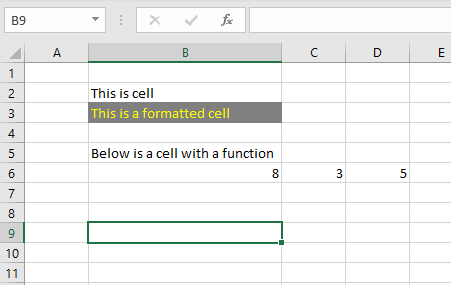
\includegraphics[width=1.2\textwidth,height=\textheight]{./images/excel-spreadsheet.png}

}

\caption{Example entries from an Excel spreadsheet}

\end{figure}

Cell B6 contains a simple formula: \texttt{=\ C6\ +\ D6}. This formula
adds cells \texttt{C6} and \texttt{D6} resulting in the sum, 8. In
formulas, mathematical operators can be used (\(+, -, \times , \div\) ).
Formulas can be also extended with inbuilt function such as showed in
Table~\ref{tbl-excelfunctions}.

\hypertarget{tbl-excelfunctions}{}
\begin{longtable}[]{@{}lll@{}}
\caption{\label{tbl-excelfunctions}Often used functions in
excel}\tabularnewline
\toprule\noalign{}
Function & English & Norwegian \\
\midrule\noalign{}
\endfirsthead
\toprule\noalign{}
Function & English & Norwegian \\
\midrule\noalign{}
\endhead
\bottomrule\noalign{}
\endlastfoot
Sum & \texttt{SUM()} & \texttt{SUMMER()} \\
Average & \texttt{AVERAGE()} & \texttt{GJENNOMSNITT()} \\
Standard deviation & \texttt{STDEV.S()} & \texttt{STDEV.S()} \\
Count & \texttt{COUNT()} & \texttt{ANTALL()} \\
Intercept & \texttt{INTERCEPT()} & \texttt{SKJÆRINGSPUNKT()} \\
Slope & \texttt{SLOPE()} & \texttt{STIGNINGSTALL()} \\
If & \texttt{IF()} & \texttt{HVIS()} \\
\end{longtable}

The sum, average, standard deviation, and count are simple functions for
summarizing data. Intercept and slope are functions used to get simple
associations from two sets of numbers (based on a regression model). The
IF function is an example of a function that can be used to enter data
in a cell conditionally. For example, IF cell A1 contains a certain
number, then cell B1 should display another specified text.

When looking for tips and tricks online, you may come across functions
for excel in other languages than what is installed on your computer. To
translate functions and for a complete overview of functions included in
Microsoft Excel, see this website
\href{https://en.excel-translator.de/}{en.excel-translator.de/}.

\hypertarget{tidy-data-and-data-storage}{%
\section{Tidy data and data storage}\label{tidy-data-and-data-storage}}

Hadley Wickham (the author of many commonly used R packages) quotes
Tolstoy when describing the principle of tidy data (Wickham 2014). This
quote is so famous that it has given name to a principle. The principle
in turn comes in many variants but basically states that when something
goes wrong, it can be wrong in multiple ways. But when it is
right/correct/works/succeeds, it does so in only one way\footnote{See
  https://en.wikipedia.org/wiki/Anna\_Karenina\_principle}. This
principle can be applied to data sets. There are so many ways that
formatting of data sets can be problematic, but a limited set of
principles makes it good.

\begin{figure}

{\centering \includegraphics[width=0.5\textwidth,height=\textheight]{index_files/mediabag/800px-Leon_tolstoi.jpg}

}

\caption[Leo Tolstoy]{Leo Tolstoy at the time when he was (possibly)
authoring Anna Karenina. (Source:
https://en.wikipedia.org/wiki/Leo\_Tolstoy)}

\end{figure}

A tidy data set consists of \emph{values} originating from
\emph{observations} and belonging to \emph{variables}. A variable is a
definition of the values based on attributes. An observation may consist
of several variables (Wickham 2014).

A tidy data set typically has one observation per row and one variable
per column. Let's say that we want to collect data from a strength test.
A participant (\textbf{participant} is a variable) in our study conducts
tests before and after the intervention (\textbf{time} is a variable) in
two exercises (\textbf{exercise} is a variable), and we record the
maximal strength in kg (\textbf{load} is a variable). The data set will
look like the table below (Table~\ref{tbl-tidydata}).

\hypertarget{tbl-tidydata}{}
\begin{longtable}[]{@{}llll@{}}
\caption{\label{tbl-tidydata}Example of tidy data}\tabularnewline
\toprule\noalign{}
Participant & Time & Exercise & Load \\
\midrule\noalign{}
\endfirsthead
\toprule\noalign{}
Participant & Time & Exercise & Load \\
\midrule\noalign{}
\endhead
\bottomrule\noalign{}
\endlastfoot
Bruce Wayne & pre & Bench press & 95 \\
Bruce Wayne & post & Bench press & 128 \\
Bruce Wayne & pre & Leg press & 180 \\
Bruce Wayne & post & Leg press & 280 \\
\end{longtable}

Another example contains variables that actually carries two pieces of
information in one variable. We again did a strength test, this time as
maximal isometric contractions and in each test consisted of two
attempts. We record this in two different variables, attempt 1 and 2.
The resulting data set could look something like in Table
Table~\ref{tbl-tidydata2}.

\hypertarget{tbl-tidydata2}{}
\begin{longtable}[]{@{}lllll@{}}
\caption{\label{tbl-tidydata2}Another example of tidy
data.}\tabularnewline
\toprule\noalign{}
Participant & Time & Exercise & Attempt1 & Attempt2 \\
\midrule\noalign{}
\endfirsthead
\toprule\noalign{}
Participant & Time & Exercise & Attempt1 & Attempt2 \\
\midrule\noalign{}
\endhead
\bottomrule\noalign{}
\endlastfoot
Selina Kyle & pre & Isometric & 81.3 & 92.5 \\
Selina Kyle & post & Isometric & 97.1 & 114.1 \\
\end{longtable}

To make this data set tidy we need to extract the attempt information
and record it in another variable as seen in Table~\ref{tbl-tidydata3}.

\hypertarget{tbl-tidydata3}{}
\begin{longtable}[]{@{}lllll@{}}
\caption{\label{tbl-tidydata3}A third example of tidy
data.}\tabularnewline
\toprule\noalign{}
Participant & Time & Exercise & Attempt & load \\
\midrule\noalign{}
\endfirsthead
\toprule\noalign{}
Participant & Time & Exercise & Attempt & load \\
\midrule\noalign{}
\endhead
\bottomrule\noalign{}
\endlastfoot
Selina Kyle & pre & Isometric & 1 & 81.3 \\
Selina Kyle & pre & Isometric & 2 & 92.5 \\
Selina Kyle & post & Isometric & 1 & 97.1 \\
Selina Kyle & post & Isometric & 2 & 114.1 \\
\end{longtable}

This transformation naturally gives additional rows to the data set. It
is sometimes referred to as ``long format'' data instead of the
structure where each attempt is given separate variables, called ``wide
format.'' You will notice during the course that the long format is most
convenient for most purposes. This is true when we create graphs and do
statistical modeling. But sometimes, a variable must be structured in a
wide format to allow certain operations.

If we follow what is recommended by Broman and Woo (Broman and Woo
2018), it is clear that each cell in a spreadsheet should only contain
one value. If we, for example, decide to format a cell to a certain
color, we add data to that cell on top of the actual data. You might add
color to a cell to remember to add or change data. However, this
information is lost when you use the data set in other software.
Instead, you should add another variable to allow such data to be
properly recorded. Using a variable called \texttt{comments}, you can
add text describing information about that particular observation,
information that is not lost when you use the data set in another
software.

\hypertarget{recording-data}{%
\section{Recording data}\label{recording-data}}

A trade secret\footnote{A trade secret as in ``not generally known to
  the public''. See
  \href{https://en.wikipedia.org/wiki/Trade_secret}{en.wikipedia.org/wiki/Trade\_secret}.}
from people who work all day with data and programming is that they are
lazy. Lazy in the sense that you want to type as little as possible and
avoid moving your arm to the computer mouse whenever possible. When
recording data, we can be lazy too. We can do this by shortening
variable names and not using CAPITAL letters when entering text in data
storage. After a hard day at the keyboard, you will be happy to write
\texttt{strtest} instead of \texttt{Strength\ Test}. The extra effort of
using two capital letters might be the thing to tip you over the
edge\footnote{In the movie Falling Down, Michael Douglas plays a
  unemployed engineer who gets push over edge, would it have been enough
  with a few to many capital letters?}. However, we should not be too
lazy either; variable names and values should be ``short but
meaningful'' (Broman and Woo 2018).

\begin{figure}

{\centering \includegraphics[width=0.5\textwidth,height=\textheight]{index_files/mediabag/Falling_Down_-1993_f.jpg}

}

\caption[Michael Douglas in Falling Down]{D-FENS Foster gets pushed over
the edge (Source: https://en.wikipedia.org/wiki/Falling\_Down)}

\end{figure}

Data and variables should also be consistent. Do not mix data type; use
a consistent way of entering e.g., dates and time, and do not use spaces
or special characters. To enforce this, you might want to start your
data collection by writing up a data dictionary describing all variables
you collect. The dictionary can set the rules for your variables. This
dictionary can also guide your data validation.

In Excel, you can use data validation to set rules for data entry. For
example, if you have a numeric variable, you can set Excel only to
accept numbers in a specified set of cells. Such rules make it harder to
enter erroneous data.

\hypertarget{saving-data}{%
\section{Saving data}\label{saving-data}}

Data from spreadsheets can be saved as special spreadsheet files, such
as \texttt{.xlsx}. This format allows for functions, multiple
spreadsheets in the same file (tabs), and cell formatting. You do not
need this fancy format if you follow the tips described above and in
(Broman and Woo 2018). Instead, you can store your data as a
\texttt{.csv} file. This format may be read and edited with Excel (or
another spreadsheet software) and in plain text. Data entered in this
format (comma-separated values; csv) can look like this in a text
editor:

\begin{verbatim}
 Participant;Time;Exercise;Attempt;load
 Selina Kyle;pre;Isometric;1;81.3  
 Selina Kyle;pre;Isometric;2;92.5
 Selina Kyle;post;Isometric;1;97.1
 Selina Kyle;post;Isometric;2;114.1
\end{verbatim}

This format is quite lovely. The data takes little space; the simple
format requires that data is well documented using e.g., a data
dictionary; and it is available for many other software as the format is
simple. You can document the data using a \texttt{README} file that
could describe the purpose and methods of data collection, how the data
is structured, and what kind of data the variables contains. A simple
\texttt{README} file can be written in a text editor such as Notepad and
saved as a \texttt{.txt} file. Later in this course, we will introduce a
``markup'' language often used to create \texttt{README} files
containing a syntax that formats the text to a more pleasant style when
converted to other formats.

\hypertarget{references-and-footnotes-1}{%
\section{References and footnotes}\label{references-and-footnotes-1}}

\bookmarksetup{startatroot}

\hypertarget{getting-to-know-r-and-rstudio}{%
\chapter{Getting to know R and
RStudio}\label{getting-to-know-r-and-rstudio}}

In \protect\hyperlink{introduction-to-data-science}{Chapter 2}, we went
through all the trouble of installing and setting up the tools needed to
become data scientists. It is now assumed that everything was indeed
installed and working. In this chapter we will introduce the usage of R
and Rstudio. First we will set up and customize RStudio and then learn
how to communicate with R.

\hypertarget{the-anatomy-of-rstudio}{%
\section{The Anatomy of RStudio}\label{the-anatomy-of-rstudio}}

The appearance of RStudio can be changed for a more pleasant user
experience. I like a dark theme as it is easier on the eye. We can also
move the different components of RStudio. I like to have The console on
the top right and the source on the top left. I think this makes it
easier to see output when coding interactively.

All this will be clearer as thing evolve, but for now, start R Studio,
go to Tools \textgreater{} Global options and make it personal (see
Figure~\ref{fig-customize})!

\begin{figure}

{\centering \includegraphics{images/ch3/03-customizerstudio.gif}

}

\caption{\label{fig-customize}Customize the appearance of RStudio}

\end{figure}

As you may have spotted in the image above, it is possible to change the
font of your editor. I like
\href{https://github.com/tonsky/FiraCode/wiki/RStudio-instructions}{Fira
code}.

\begin{tcolorbox}[enhanced jigsaw, coltitle=black, titlerule=0mm, colframe=quarto-callout-tip-color-frame, colbacktitle=quarto-callout-tip-color!10!white, opacitybacktitle=0.6, breakable, left=2mm, opacityback=0, bottomtitle=1mm, bottomrule=.15mm, colback=white, toptitle=1mm, arc=.35mm, title=\textcolor{quarto-callout-tip-color}{\faLightbulb}\hspace{0.5em}{Defining concepts}, leftrule=.75mm, toprule=.15mm, rightrule=.15mm]

\textbf{Source editor}: Is where scripts are edited.

\textbf{Environment}: In R, the environment is where data variables and
structures are saved during execution of code.

\textbf{Script}: Your script is the document containing your computer
code. This is your computer program (using a loose definition of a
software program).

\textbf{Variables}: In R, variables are containers for data values.

\textbf{Workspace}: This is your environments as represented on your
computer. A workspace can be, but should not be saved between sessions.

\end{tcolorbox}

\hypertarget{the-source-editor}{%
\subsection{The source editor}\label{the-source-editor}}

The source editor is where you edit your code. When writing your code in
a text-file, you can call it a script, this is essentially a computer
program where you tell R what to do. It is executed from top to bottom.
You can send one line of code, multiple lines or whole sections into R.
In the image below (Figure~\ref{fig-interactionrstudio}), the source
window is in the top left corner.

\hypertarget{environment}{%
\subsection{Environment}\label{environment}}

The environment is where all your objects are located. Objects can be
variables or data sets that you are working with. In RStudio the
environment is listed under the environment tab (bottom left in the
image).

Copy the code below to a R script. To run it line by line, set your
cursor on the first line a press Ctrl+Enter.What happened in your
environment? Press Ctrl+Enter again and you will see a plot in the plot
window. Amazing stuff!

\begin{Shaded}
\begin{Highlighting}[numbers=left,,]
\NormalTok{a }\OtherTok{\textless{}{-}} \FunctionTok{c}\NormalTok{(}\DecValTok{1}\NormalTok{, }\DecValTok{2}\NormalTok{, }\DecValTok{3}\NormalTok{, }\DecValTok{4}\NormalTok{)}

\FunctionTok{plot}\NormalTok{(a)}
\end{Highlighting}
\end{Shaded}

\hypertarget{the-console}{%
\subsection{The console}\label{the-console}}

By pressing Ctrl+Enter from the script, as described above, you sent
your code to the console. You can also interact with R directly here. By
writing \texttt{a} in the console and hitting enter you will get the
value from the object called a. This means that it is also where output
from R is usually printed. In the image below, the console is in the top
right corner.

\hypertarget{files-plots-packages-and-help-files}{%
\subsection{Files, plots, packages and help
files}\label{files-plots-packages-and-help-files}}

In RStudio files are accessible from the Files tab. The files tab shows
the files in you root folder. The root folder is where R will search for
files if you tell it to. We will talk more about the root folder later
in connection with projects. Plots are displayed in the Plot tab.
Packages are listed in the packages tab. If you access the help files,
these will be displayed in the help tab. In the image below all these
tabs are in the bottom right corner. More on help files and packages
later.

\begin{figure}

{\centering \includegraphics{images/ch3/03-interactingrstudio.gif}

}

\caption{\label{fig-interactionrstudio}Interacting with RStudio}

\end{figure}

\hypertarget{reproducible-data-science-using-rstudio}{%
\section{Reproducible data science using
RStudio}\label{reproducible-data-science-using-rstudio}}

When starting to work more systematically in RStudio we will set some
rules that will allow for reproducible programming. Remember from
\protect\hyperlink{replication-and-reproducibility}{Chapter 2} that part
of a fully reproducible study is software/code that produces the
results. It turns out that when working interactively with R you can
fool yourself to belive that you have included all steps needed to
produce some results in your script. However, variables may be stored in
your environment but not by assigning values to them in your script.
This will become a problem if you want to share your code, a certain
value/variable needed to make the program work may be missing from your
script.

To avoid making such a mistake it is good practice not to save variables
in your environment between sessions, everything should be scripted and
documented and assumed not defined elsewhere. In RStudio we can make an
explicit setting Not to save the workspace (See
Figure~\ref{fig-saveworkspace}).

\begin{figure}

{\centering \includegraphics{images/ch3/03-ask-workspace.gif}

}

\caption{\label{fig-saveworkspace}Never save the workspace.}

\end{figure}

\hypertarget{basics-r-programming-installing-and-using-swirl}{%
\section{\texorpdfstring{Basics R programming, Installing and using
\texttt{swirl}}{Basics R programming, Installing and using swirl}}\label{basics-r-programming-installing-and-using-swirl}}

Swirl is a great way to get to know how to talk with R. Swirl consists
of lessons created for different topics. Install swirl by typing the
following into your console:

\begin{Shaded}
\begin{Highlighting}[numbers=left,,]
\FunctionTok{install.packages}\NormalTok{(}\StringTok{"swirl"}\NormalTok{)}
\end{Highlighting}
\end{Shaded}

When \texttt{swirl}is installed you will need to load the package This
means that all functions that are included in package becomes available
to you in your R session. To load the package you use the
\texttt{library} function.

\begin{Shaded}
\begin{Highlighting}[numbers=left,,]
\FunctionTok{library}\NormalTok{(}\StringTok{"swirl"}\NormalTok{)}
\end{Highlighting}
\end{Shaded}

When you run the above command in your console you will get a message
saying to call \texttt{swirl()} when you are ready to learn. I would
like you to run the course ``R Programming: The basics of programming in
R''. Swirl will ask if you want to install it. After installation, just
follow the instructions in the console. To get out of swirl, just press
ESC.

\hypertarget{file-formats-for-editing-and-executiong-r-code}{%
\section{File formats for editing and executiong R
code}\label{file-formats-for-editing-and-executiong-r-code}}

\hypertarget{r-scripts}{%
\subsection{R scripts}\label{r-scripts}}

RStudio has capabilities to highlight code for multiple languages. We
will focus on R. The most basic file format for R code is an R script,
as we have already touched upon. An R script contains code and comments.
Code is executed by R and comments are ignored. Ideally, R scripts are
commented to improve readability of what the do. Commenting code is also
a good way of creating a roadmap of what you want to do. In the image
below (Figure~\ref{fig-rscript}), R code is written based on a plan
written with comments. Note that when a line starts with at least one
\texttt{\#} it is interpreted by R as a comment.

\begin{figure}

{\centering \includegraphics{images/ch3/03-rscript.gif}

}

\caption{\label{fig-rscript}Commenting and coding in an R script}

\end{figure}

Try the code for yourself to see what it produces. The details will be
covered later.

\begin{Shaded}
\begin{Highlighting}[numbers=left,,]
\DocumentationTok{\#\# Create two vectors of random numbers}
\NormalTok{x }\OtherTok{\textless{}{-}} \FunctionTok{rnorm}\NormalTok{(}\DecValTok{10}\NormalTok{, }\DecValTok{0}\NormalTok{, }\DecValTok{1}\NormalTok{)}
\NormalTok{y }\OtherTok{\textless{}{-}} \FunctionTok{rnorm}\NormalTok{(}\DecValTok{10}\NormalTok{, }\DecValTok{10}\NormalTok{, }\DecValTok{10}\NormalTok{)}

\DocumentationTok{\#\# Create an x{-}y plot of the two vectors}
\FunctionTok{plot}\NormalTok{(x, y)}
\end{Highlighting}
\end{Shaded}

\hypertarget{r-markdown-and-quarto-files}{%
\subsection{R markdown and quarto
files}\label{r-markdown-and-quarto-files}}

The more advanced file formats for R are RMarkdown (\texttt{.rmd}) and
quarto (\texttt{.qmd}) files. These have the capabilities of combining
formatted text with computer code. The source document may contain
multiple pieces of code organized in code chunks together with text
formatted with markdown syntax. A meta data field in the top of the
source file specifies settings for the conversion to output formats.
Multiple output formats are available, including HTML, word and PDF. The
image below shows the basic outline of a very simple quarto file
destined to create a HTML document.

Notice also that RStudio offers an visual editor where the output is
approximated and formatting is available from a menu.

Adding headlines and makes it possible to navigate the document through
the outline or the list of components in the bottom of the document.

\begin{figure}

{\centering \includegraphics{images/ch3/03-quartoauthor.gif}

}

\caption{Authoring in a quarto source document and preview in the visual
editor}

\end{figure}

\href{https://rmarkdown.rstudio.com/}{R markdown} and
\href{https://quarto.org/docs/guide/}{quarto} have many similarities as
the basic organization is similar between the two. The text parts are
written using a special syntax, markdown. The point of markdown is that
you will use the same syntax that is later possible to convert to
multiple formats. The syntax let's you do all formatting explicitly, for
example instead of getting your mouse to superscript some text you can
add syntax \texttt{a\^{}2\^{}} to achieve a\textsuperscript{2}.

A full guide to RMarkdown can be found on the official
\href{https://rmarkdown.rstudio.com/lesson-1.html}{R markdown web
pages}. I suggest you take the time to get an overview of this language
as it will make you more fluent in the tools that enables reproducible
computing. When writing R markdown, it is handy to have a \emph{cheat
sheet} close by when writing,
\href{https://www.rstudio.com/wp-content/uploads/2015/02/rmarkdown-cheatsheet.pdf}{here
is an example for Rmarkdown}, and here is
\href{https://rstudio.github.io/cheatsheets/html/quarto.html}{another
one for quarto} \footnote{Cheat sheets are available in R Studio:
  \emph{Help \textgreater{} Cheatsheets}}.

\hypertarget{microsoft-word-intergration-in-r-markdown-and-quarto}{%
\subsubsection{Microsoft Word intergration in R Markdown and
Quarto}\label{microsoft-word-intergration-in-r-markdown-and-quarto}}

Sometimes it is useful to ``knit'' to a word file. For example when you
want to share a report with fellow students who are not familiar with R.
R Markdown/Quarto can be used as a source for word documents (.docx).

To create a word document from your Rmd-file/qmd-file you need a working
installation of Microsoft Word. Settings for the output is specified in
the YAML metadata field in the Rmd-file. This is the first section of a
Rmd file, and when you want it to create a word file you specify it like
this:

\begin{verbatim}
---
title: "A title"
author: Daniel Hammarström
date: 2020-09-05
output: word_document
---
\end{verbatim}

The \texttt{output:\ word\_document} (or \texttt{format:\ docx} when
using quarto) tells R to create a word file. If you are not happy with
the style of the word document (e.g.~size and font of text) you can tell
R to use a template file. Save a word file that you have knitted as
\texttt{reference.docx} and use specify in the YAML field that you will
use this as reference.
\href{https://quarto.org/docs/reference/formats/docx.html}{See here for
the equivalent formatting of quarto documents}

\begin{verbatim}
---
title: "A title"
author: Daniel Hammarström
date: 2020-09-05
output: 
        word_document:
                reference_docx: reference.docx
---
\end{verbatim}

Edit styles (Stiler in Norwegian) used in the reference file (right
click on the style and edit). For example, editing the ``Title'' style
(Tittel in Norwegian) will change the main titel of the document. After
you have edited the document, save it.

When you knit the document again, your updated styles will be used your
word document.

\href{https://rmarkdown.rstudio.com/articles_docx.html}{Here} you can
read more about using R Markdown together with word. If you do not have
word installed, you can also use Open Office. Read more about it
\href{https://bookdown.org/yihui/rmarkdown/opendocument-text-document.html}{here}.

\hypertarget{adding-references-to-r-markdown-and-quarto-files}{%
\subsubsection{Adding references to R Markdown and Quarto
files}\label{adding-references-to-r-markdown-and-quarto-files}}

References/citations can be added to the report using the
\texttt{bibliography} option in the YAML field. Citations needs to be
listed in a file, multiple formats are availiable. A convenient format
is bibtex. When using this format, create a text file with the ending
\texttt{.bib}, for example, \texttt{bibliography.bib}.

The \texttt{bibliography.bib}-file needs to be activated in the
YAML-field. Do it by adding this information:

\begin{verbatim}
---
title: "A title"
author: Daniel Hammarström
date: 2020-09-05
output: 
        word_document:
                reference_docx: reference.docx
bibliography: bibliography.bib
---
\end{verbatim}

Add citations to the file in bibtex-format. Here is an example:

\begin{verbatim}
@Article{refID1,
   Author="Ellefsen, S.  and Hammarstrom, D.  and Strand, T. A.  and Zacharoff, E.  and Whist, J. E.  and Rauk, I.  and Nygaard, H.  and Vegge, G.  and Hanestadhaugen, M.  and Wernbom, M.  and Cumming, K. T.  and Rønning, R.  and Raastad, T.  and Rønnestad, B. R. ",
   Title="{Blood flow-restricted strength training displays high functional and biological efficacy in women: a within-subject comparison with high-load strength training}",
   Journal="Am. J. Physiol. Regul. Integr. Comp. Physiol.",
   Year="2015",
   Volume="309",
   Number="7",
   Pages="R767--779",
   Month="Oct"}
\end{verbatim}

The part that says \texttt{refID1} can be edited to something
appropriate. This is a reference identification, you use it to get the
citation into the text. When citing you do it in the form

\begin{verbatim}
Blood flow-restricted training leads to similar adaptations as traditional training [@refID1].
\end{verbatim}

This will appear in text as:

\begin{quote}
Blood flow-restricted training leads to similar adaptations as
traditional training (Ellefsen et al. 2015).
\end{quote}

The reference will end up in the end of the document (as on this
webpage).

You can gather references in bibtex format from Oria (use the BIBTEX
icon) and from PubMed using
\href{https://www.bioinformatics.org/texmed/}{TeXMed}. You can also
export reference in bibtex format from citation software like Endnote or
Zotero. Make sure you check all references when entering them,
especially MedTex gives some problems with ``scandinavian'' letters (å æ
ä ø ö).

Recently RStudio added support for adding citations inside the visual
markdown editor.

\hypertarget{packages}{%
\section{Packages}\label{packages}}

The R ecosystem consists of packages. These are \emph{functions}
organized in a systematic manner. Functions are created to perform a
specialized task. And packages often have many function used to do
e.g.~analyses of a specific kind of data, or more general task such as
making figures or handle data.

In this course we will use many different packages, for example
\href{https://dplyr.tidyverse.org/}{dplyr},
\href{https://tidyr.tidyverse.org/}{tidyr} and
\href{https://ggplot2.tidyverse.org/}{ggplot2}. dplyr and tidyr are
packages used to transform and clean data. ggplot2 is used for making
figures.

To install a package, you use the \texttt{install.packages()} function.
You only need to do this once on your computer (unless you re-install
R). You can write the following code in your console to install dplyr.

\begin{Shaded}
\begin{Highlighting}[numbers=left,,]
\FunctionTok{install.packages}\NormalTok{(}\StringTok{"dplyr"}\NormalTok{)}
\end{Highlighting}
\end{Shaded}

Alternatively, click ``Packages'' and ``Install'' and search for the
package you want to install. To use a package, you have to load it into
your environment. Use the \texttt{library()} function to load a package.

\begin{Shaded}
\begin{Highlighting}[numbers=left,,]
\FunctionTok{library}\NormalTok{(}\StringTok{"dplyr"}\NormalTok{)}
\end{Highlighting}
\end{Shaded}

\hypertarget{references-and-footnotes-2}{%
\section{References and footnotes}\label{references-and-footnotes-2}}

\bookmarksetup{startatroot}

\hypertarget{creating-your-first-graph}{%
\chapter{Creating your first graph}\label{creating-your-first-graph}}

Data visualization is an efficient way to understand data. Using graphs,
we can communicate characteristics of a data set in a way that would
have been impossible with a limited number of summary statistics, such
as the mean and standard deviation. In Chapter 2 of his book
(Spiegelhalter 2019), Spiegelhalter touches upon this fact when he
describes different types of graphs and their use to understand various
data sets. An important argument for mastering data visualization is
understanding what variables might explain variation in a given data set
(Spiegelhalter 2019). In this sense, data visualization can be thought
of as an initial step in understanding data; data visualization is an
exploratory tool.

RStudio is a powerful environment for data visualization. Together with
R (which is excellent for creating graphs), you can create and preview
figures that represent your data in RStudio.

R has got several systems for creating figures, plots, graphs. In this
course, we will use \href{https://ggplot2.tidyverse.org/}{ggplot2}.
Another system for plotting comes with the base installation of R. This
is sometimes referred to as base R
(\href{https://rstudio-pubs-static.s3.amazonaws.com/84527_6b8334fd3d9348579681b24d156e7e9d.html}{see
this tutorial}, or
\href{http://www.sthda.com/english/wiki/r-base-graphs}{this}. Another
well described and used system is
\href{https://www.statmethods.net/advgraphs/trellis.html}{lattice}. We
choose ggplot2 because it works well with the
\href{https://www.tidyverse.org/}{tidyverse}, and it is well described.

\hypertarget{resources}{%
\section{Resources}\label{resources}}

There are several good resources aimed at ggplot2:

\begin{itemize}
\tightlist
\item
  \href{https://r4ds.hadley.nz/data-visualize}{Chapter 2 in R for data
  science}
\item
  \href{https://ggplot2-book.org/}{The ggplot2 book}
\item
  \href{https://github.com/rstudio/cheatsheets/raw/master/data-visualization-2.1.pdf}{The
  ggplot2 cheatsheet}
\end{itemize}

\hypertarget{learning-objectives}{%
\section{Learning objectives}\label{learning-objectives}}

After working through this chapter, you should be able to answer:

\begin{itemize}
\tightlist
\item
  What are geoms?
\item
  What is mapping data to aesthetics?
\item
  What are theme components?
\end{itemize}

You should also be able to create your first graph.

\hypertarget{prerequisites-1}{%
\section{Prerequisites}\label{prerequisites-1}}

To follow the exercises below you will need to some data. For the
purpose of this course, I have created a package that contains the data
sets we need. In this chapter we will work with the
\texttt{cyclingstudy} data set. To install the package
(\texttt{exscidata}) you will need another package called
\texttt{remotes}.

The code below first checks if the package \texttt{remotes} is
installed, or more specifically, if \texttt{"remotes"} cannot be found
in the list of installed packages. Using the \texttt{if} function makes
\texttt{install.packages(remotes)} conditional. If we do not find
\texttt{"remotes"} among installed packages, then install
\texttt{remotes}.

The next line of code does the same with the \texttt{exscidata} package.
However, since the package is not on CRAN but hosted on GitHub we will
need to use \texttt{remotes} to install it. The part of the second line
of code that says
\texttt{remotes::install\_github("dhammarstrom/exscidata")} uses the
function \texttt{install\_github} without loading the remotes package.
The last line of the code below loads the package \texttt{exscidata}
using the \texttt{library} function.

\begin{Shaded}
\begin{Highlighting}[numbers=left,,]
\CommentTok{\# Check if remotes is not installed, if TRUE, install remotes}
\ControlFlowTok{if}\NormalTok{ (}\SpecialCharTok{!}\StringTok{"remotes"} \SpecialCharTok{\%in\%} \FunctionTok{installed.packages}\NormalTok{()) }\FunctionTok{install.packages}\NormalTok{(remotes)}

\CommentTok{\# Check if exscidata is not installed, if TRUE, install exscidata from github}
\ControlFlowTok{if}\NormalTok{ (}\SpecialCharTok{!}\StringTok{"exscidata"} \SpecialCharTok{\%in\%} \FunctionTok{installed.packages}\NormalTok{()) remotes}\SpecialCharTok{::}\FunctionTok{install\_github}\NormalTok{(}\StringTok{"dhammarstrom/exscidata"}\NormalTok{)}

\CommentTok{\# Load exscidata}
\FunctionTok{library}\NormalTok{(exscidata)}
\end{Highlighting}
\end{Shaded}

Next we need to load the \texttt{tidyverse} package. This package in
turn loads several packages that we will use when transforming data and
making our figures. I will include the line of code that checks if the
package is installed, if not, R will download and install it. We
subsequently load the package using \texttt{library}.

\begin{Shaded}
\begin{Highlighting}[numbers=left,,]
\CommentTok{\# Check if tidyverse is not installed, if TRUE, install remotes}
\ControlFlowTok{if}\NormalTok{ (}\SpecialCharTok{!}\StringTok{"tidyverse"} \SpecialCharTok{\%in\%} \FunctionTok{installed.packages}\NormalTok{()) }\FunctionTok{install.packages}\NormalTok{(tidyverse)}

\FunctionTok{library}\NormalTok{(tidyverse)}
\end{Highlighting}
\end{Shaded}

\begin{verbatim}
-- Attaching core tidyverse packages ------------------------ tidyverse 2.0.0 --
v dplyr     1.1.2     v readr     2.1.4
v forcats   1.0.0     v stringr   1.5.0
v ggplot2   3.4.2     v tibble    3.2.1
v lubridate 1.9.2     v tidyr     1.3.0
v purrr     1.0.1     
-- Conflicts ------------------------------------------ tidyverse_conflicts() --
x dplyr::filter() masks stats::filter()
x dplyr::lag()    masks stats::lag()
i Use the conflicted package (<http://conflicted.r-lib.org/>) to force all conflicts to become errors
\end{verbatim}

We are now ready to explore the data set. But first we should talk about
the main components of the \texttt{ggplot2} system.

\hypertarget{the-ggplot2-system}{%
\section{\texorpdfstring{The \texttt{ggplot2}
system}{The ggplot2 system}}\label{the-ggplot2-system}}

When using the ggplot2 system we can think of the resulting graph as
containing data that has been \emph{mapped} to different coordinates,
colors, shapes, sizes, and other attributes that determine what is being
visualized. We are using different geometric representations of the data
in the visualization.

When we \emph{map} data in ggplot we use a specific function,
\texttt{aes()} (short for aesthetic). We will use this inside the main
engine, \texttt{ggplot()}. For this first simple example, we will create
a data set by simulating some data. When you simulate data in R, you can
tell R what should be the starting point in the random number generator.
Using \texttt{set.seed(100)}, we can recreate the same numbers from our
``number generator'' later. In the example below, we use
\texttt{rnorm()} to simulate numbers from a normal distribution. Using
the arguments \texttt{n\ =\ 10}, \texttt{mean\ =\ 0}, and
\texttt{sd\ =\ 1}, we simulate randomly picking ten numbers from a
distribution with a mean of 0 and a standard deviation of 1. These
numbers are stored in a data frame that is assigned to an object that we
have named \texttt{dat}.

\begin{Shaded}
\begin{Highlighting}[numbers=left,,]
\CommentTok{\# Set the seed for random generation of numbers}
\FunctionTok{set.seed}\NormalTok{(}\DecValTok{100}\NormalTok{)}

\CommentTok{\# Store data in a data frame}
\NormalTok{dat }\OtherTok{\textless{}{-}} \FunctionTok{data.frame}\NormalTok{(}\AttributeTok{x =} \FunctionTok{rnorm}\NormalTok{(}\DecValTok{10}\NormalTok{, }\AttributeTok{mean =} \DecValTok{0}\NormalTok{, }\AttributeTok{sd =} \DecValTok{1}\NormalTok{), }
                  \AttributeTok{y =} \FunctionTok{rnorm}\NormalTok{(}\DecValTok{10}\NormalTok{, }\AttributeTok{mean =} \DecValTok{10}\NormalTok{, }\AttributeTok{sd =} \DecValTok{2}\NormalTok{))}
\end{Highlighting}
\end{Shaded}

The data set consists of two variables. We will start the process of
creating the graph by creating the canvas, and this basically sets the
border of the figure we want to make. The \texttt{ggplot()} function
takes the data set as its first argument, followed by the \texttt{aes()}
function that maps data to coordinates and other attributes. In this
case, we have mapped our data to the x- and y-coordinates of the figure.

\begin{Shaded}
\begin{Highlighting}[numbers=left,,]
\FunctionTok{ggplot}\NormalTok{(dat, }\FunctionTok{aes}\NormalTok{(}\AttributeTok{x =}\NormalTok{ x, }\AttributeTok{y =}\NormalTok{ y))}
\end{Highlighting}
\end{Shaded}

\begin{figure}[H]

{\centering 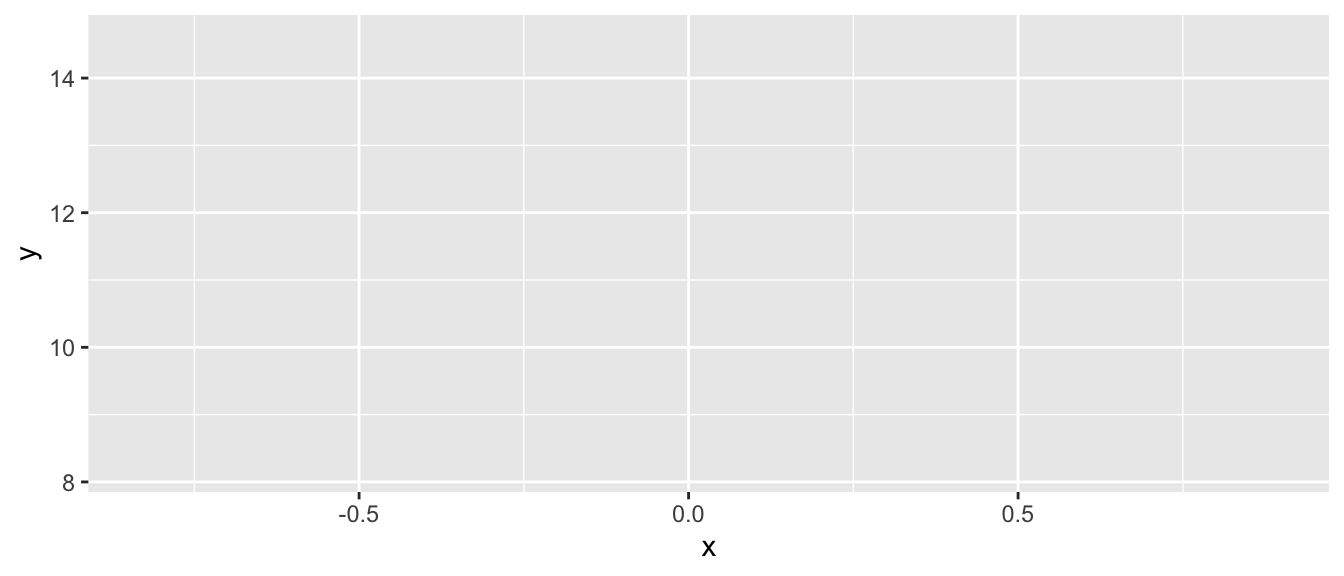
\includegraphics{04-first-graph_files/figure-pdf/fig-empty-canvas-1.pdf}

}

\caption{\label{fig-empty-canvas}An empty \texttt{ggplot} canvas.}

\end{figure}

As you can see in Figure~\ref{fig-empty-canvas}, the code above creates
an ``empty canvas'' that has enough room to visualize our data. The x-
and y-axes are adjusted to give room for graphical representations of
the data. Next we need to add geometric shapes (\texttt{geom} for
short). These are functions that we add to the plot using the \texttt{+}
sign. These functions all start with \texttt{geom\_} and has and ending
that describes the geometric shape, like for example point or line.

We will add \texttt{geom\_point()} to our empty canvas as plotted in
Figure~\ref{fig-empty-canvas}. The \texttt{geom\_point} function
\emph{inherits} the mapping from from \texttt{ggplot()}. Shapes, in this
case points will be placed according to x- and y-coordinates specified
in \texttt{aes()} used in the main \texttt{ggplot} function call. This
means that we do not need to specify anything in \texttt{geom\_point} at
this stage.

\begin{Shaded}
\begin{Highlighting}[numbers=left,,]
\FunctionTok{ggplot}\NormalTok{(dat, }\FunctionTok{aes}\NormalTok{(}\AttributeTok{x =}\NormalTok{ x, }\AttributeTok{y =}\NormalTok{ y)) }\SpecialCharTok{+} \FunctionTok{geom\_point}\NormalTok{()}
\end{Highlighting}
\end{Shaded}

\begin{figure}[H]

{\centering 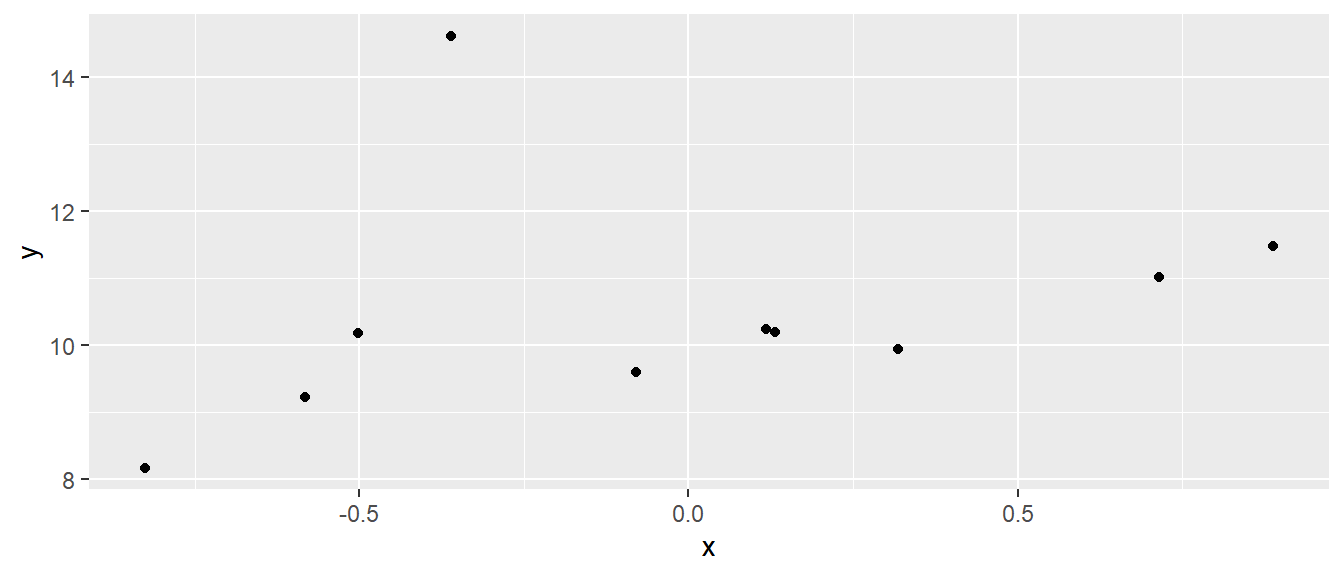
\includegraphics{04-first-graph_files/figure-pdf/fig-point-and-canvas-1.pdf}

}

\caption{\label{fig-point-and-canvas}A \texttt{ggplot} canvas with
points added.}

\end{figure}

In Figure~\ref{fig-point-and-canvas} we have added black points to each
x- and y-coordinate representing \texttt{x} and \texttt{y} from our data
set.

To extend the example we will add data to our data set. In the code
below, we create a new variable in the data set using \texttt{\$}
effectively giving us a new column in the data. We use
\texttt{rep("A",\ 5)} to replicate the letter \texttt{A} five times and
the same for \texttt{B}. The \texttt{c()} function combines the two in a
single vector. We can use \texttt{head(dat)} to see what we accomplished
with these operations. The \texttt{head()} function \emph{prints} the
first six rows from the data set.

\begin{Shaded}
\begin{Highlighting}[numbers=left,,]
\NormalTok{dat}\SpecialCharTok{$}\NormalTok{z }\OtherTok{\textless{}{-}} \FunctionTok{c}\NormalTok{(}\FunctionTok{rep}\NormalTok{(}\StringTok{"A"}\NormalTok{, }\DecValTok{5}\NormalTok{), }\FunctionTok{rep}\NormalTok{(}\StringTok{"B"}\NormalTok{, }\DecValTok{5}\NormalTok{))}

\FunctionTok{head}\NormalTok{(dat)}
\end{Highlighting}
\end{Shaded}

\begin{verbatim}
            x         y z
1 -0.50219235 10.179772 A
2  0.13153117 10.192549 A
3 -0.07891709  9.596732 A
4  0.88678481 11.479681 A
5  0.11697127 10.246759 A
6  0.31863009  9.941367 B
\end{verbatim}

We can see that we have an additional variable, \texttt{z} that contains
the letters \texttt{"A"} and \texttt{"B"}. This new variable can be used
to add more information to the plot. Let's say that we want to map the
\texttt{z} variable to different colors. We do this by adding
\texttt{color\ =\ z} to \texttt{aes}. This means that we want the z
variable to determine colors.

\begin{Shaded}
\begin{Highlighting}[numbers=left,,]
\FunctionTok{ggplot}\NormalTok{(dat, }\FunctionTok{aes}\NormalTok{(}\AttributeTok{x =}\NormalTok{ x, }\AttributeTok{y =}\NormalTok{ y, }\AttributeTok{color =}\NormalTok{ z)) }\SpecialCharTok{+} \FunctionTok{geom\_point}\NormalTok{()}
\end{Highlighting}
\end{Shaded}

\begin{figure}[H]

{\centering 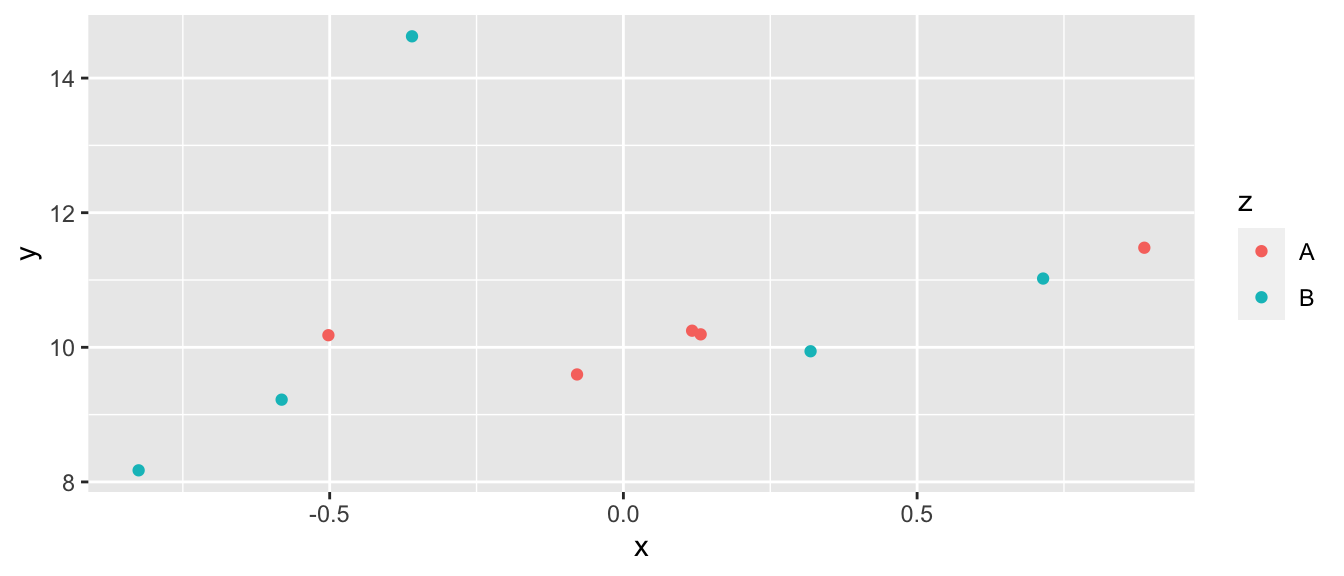
\includegraphics{04-first-graph_files/figure-pdf/fig-point-with-color-1.pdf}

}

\caption{\label{fig-point-with-color}A \texttt{ggplot} canvas with
colored points added.}

\end{figure}

In Figure~\ref{fig-point-with-color} we can see that different colors
are used for the two letters \texttt{"A"} and \texttt{"B"}. Other
attributes can also be specified like \texttt{shape}, \texttt{fill} or
\texttt{size}. The \texttt{shape} specifies the appearance of the
points. When we use use data to map to shapes, ggplot2 will start from
the standard shape.

\begin{figure}

{\centering 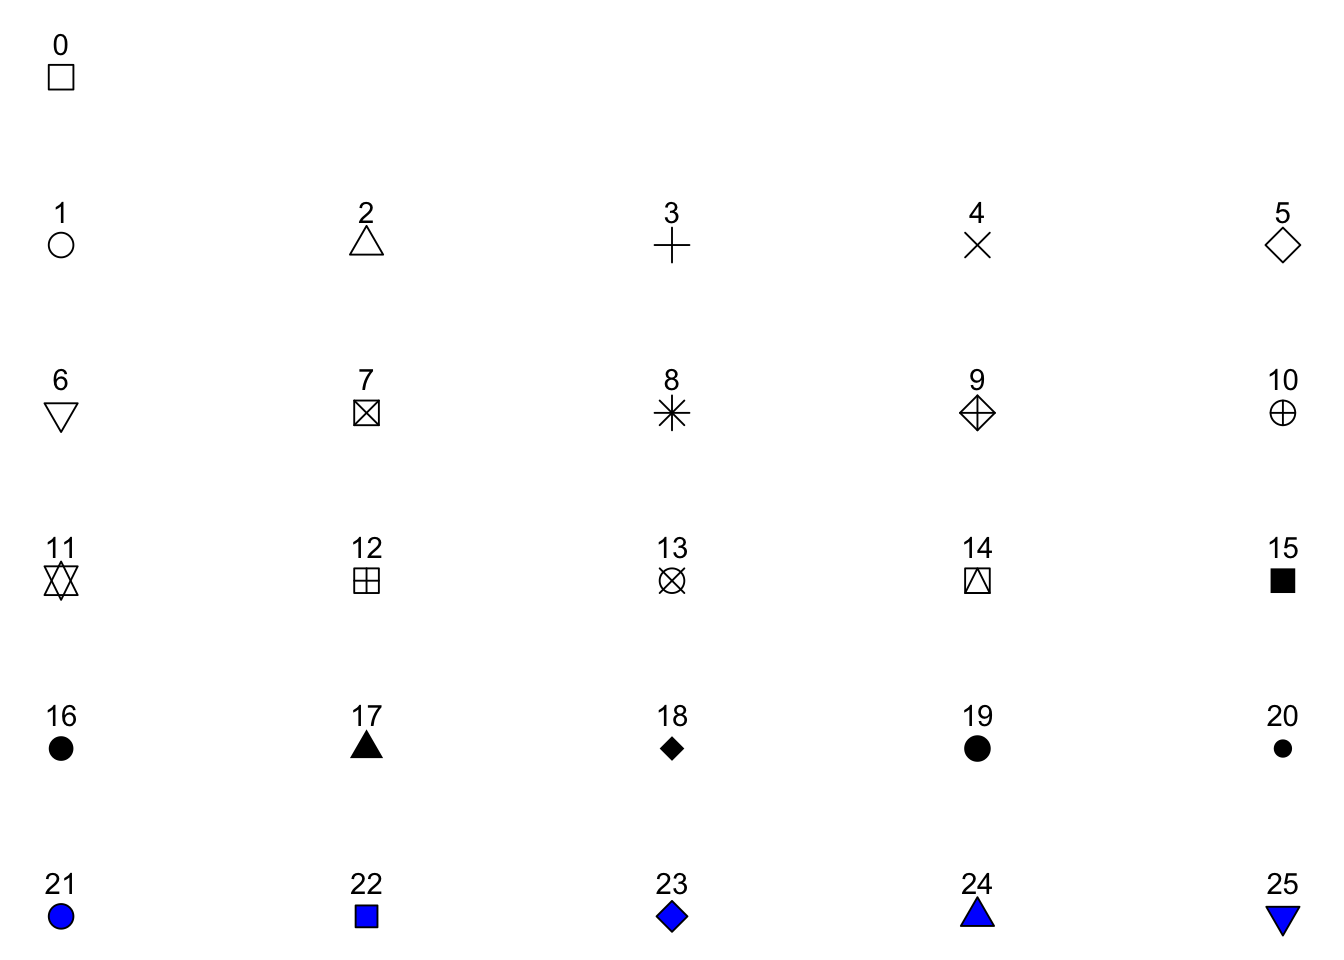
\includegraphics{04-first-graph_files/figure-pdf/fig-shapes-in-r-1.pdf}

}

\caption{\label{fig-shapes-in-r}Shapes in R}

\end{figure}

Possible shapes in the standard framework in R are shown in
Figure~\ref{fig-shapes-in-r}. Shapes 0 to 20 can change colors while
shapes 21 to 25 may have different border colors but also different fill
colors. We may use this information to change the shape, color and fill
of our points. Let's say that instead of colored points we want filled
points. We would then change the \texttt{color\ =\ z} argument to
\texttt{fill\ =\ z} and select a point shape that can be filled (shapes
21-25, see Figure~\ref{fig-shapes-in-r}. Notice in the code below that
\texttt{shape\ =\ 21} has been added to \texttt{geom\_point()}. We have
specified how points should be displayed.

\begin{Shaded}
\begin{Highlighting}[numbers=left,,]
\FunctionTok{ggplot}\NormalTok{(dat, }\FunctionTok{aes}\NormalTok{(}\AttributeTok{x =}\NormalTok{ x, }\AttributeTok{y =}\NormalTok{ y, }\AttributeTok{fill =}\NormalTok{ z)) }\SpecialCharTok{+} \FunctionTok{geom\_point}\NormalTok{(}\AttributeTok{shape =} \DecValTok{21}\NormalTok{)}
\end{Highlighting}
\end{Shaded}

\begin{figure}[H]

{\centering 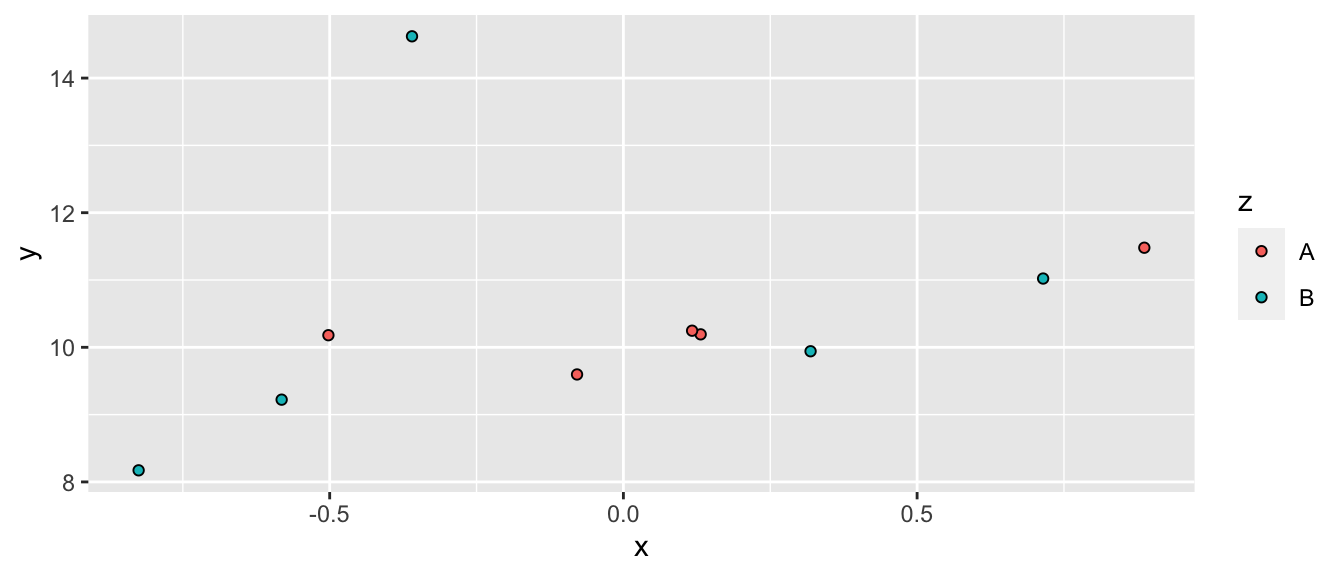
\includegraphics{04-first-graph_files/figure-pdf/fig-point-with-fill-1.pdf}

}

\caption{\label{fig-point-with-fill}A \texttt{ggplot} canvas with filled
points added.}

\end{figure}

Since shape is an attribute we can map data to it. If we want data to
determine both shape and fill we could add this information in the
\texttt{aes()} function by setting both \texttt{shape\ =\ z} and
\texttt{fill\ =\ z}. We now have to specify what shapes ggplot should
use in order to be sure we can combine both shapes and fill. We will use
\texttt{scale\_fill\_manual} and \texttt{scale\_shape\_manual} to do
this. These functions lets you specify different values for aesthetics.
Notice that we removed \texttt{shape\ =\ 21} from the
\texttt{geom\_point()} function, but we added size to increase the size
of the points (see Figure~\ref{fig-point-with-fill-and-shape}).

\begin{Shaded}
\begin{Highlighting}[numbers=left,,]
\FunctionTok{ggplot}\NormalTok{(dat, }\FunctionTok{aes}\NormalTok{(}\AttributeTok{x =}\NormalTok{ x, }\AttributeTok{y =}\NormalTok{ y, }\AttributeTok{fill =}\NormalTok{ z, }\AttributeTok{shape =}\NormalTok{ z)) }\SpecialCharTok{+} 
  \FunctionTok{geom\_point}\NormalTok{(}\AttributeTok{size =} \DecValTok{3}\NormalTok{) }\SpecialCharTok{+}
  \FunctionTok{scale\_fill\_manual}\NormalTok{(}\AttributeTok{values =} \FunctionTok{c}\NormalTok{(}\StringTok{"red"}\NormalTok{, }\StringTok{"green"}\NormalTok{)) }\SpecialCharTok{+} 
  \FunctionTok{scale\_shape\_manual}\NormalTok{(}\AttributeTok{values =} \FunctionTok{c}\NormalTok{(}\DecValTok{21}\NormalTok{, }\DecValTok{23}\NormalTok{))}
\end{Highlighting}
\end{Shaded}

\begin{figure}[H]

{\centering 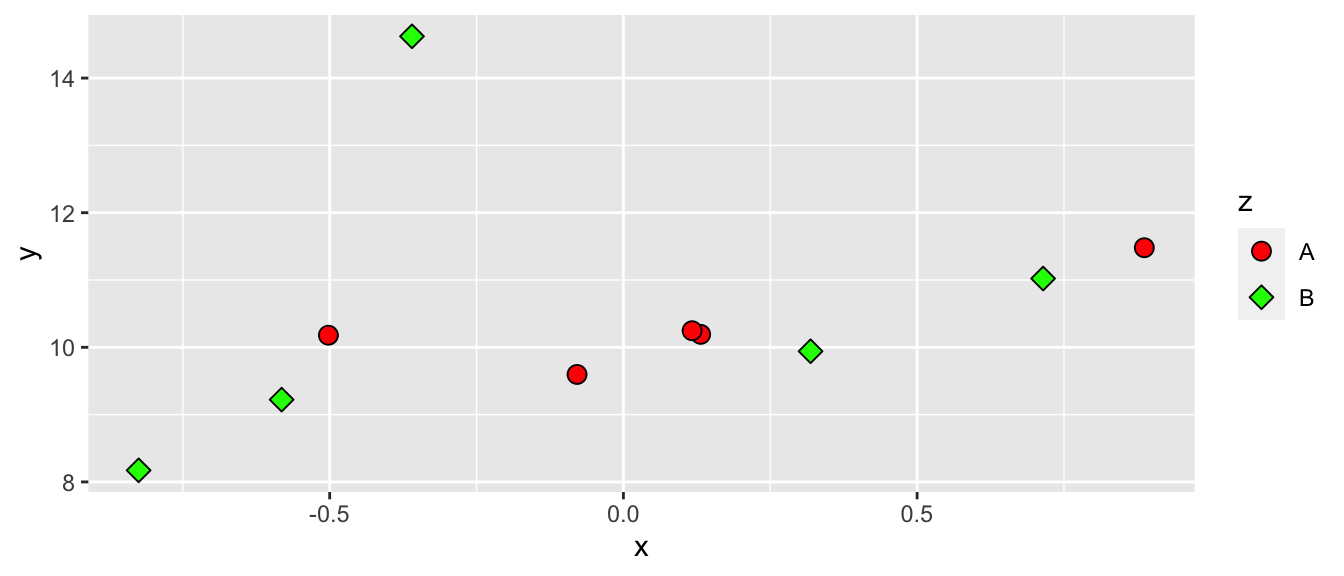
\includegraphics{04-first-graph_files/figure-pdf/fig-point-with-fill-and-shape-1.pdf}

}

\caption{\label{fig-point-with-fill-and-shape}Data mapped to fill and
shape, and size specified manually to override the default.}

\end{figure}

\hypertarget{different-geoms-using-real-data}{%
\section{Different geoms using real
data}\label{different-geoms-using-real-data}}

We have seen that the basic \texttt{ggplot2} figure maps underlying data
to coordinates and geometric representations, such as points. We will go
further by using some real data. We will be using the
\texttt{cyclingstudy} data set from the \texttt{exscidata}-package. We
will start by loading the data and select a few columns that we are
interested in.

By using \texttt{data("cyclingstudy")} we will load the data set that is
part of the \texttt{exscidata}-package to our environment. By looking at
the environment tab you can see that this operation adds a data set to
the environment. It has 80 observations and 101 variables. Using the
\texttt{glimpse()} function from \texttt{dplyr} (which is loaded by
loading \texttt{tidyverse}) we will get an overview of all variables in
the data set. I have omitted the output from the code below, feel free
to run the code in a quarto- or rmarkdown-document on your own.

\begin{Shaded}
\begin{Highlighting}[numbers=left,,]
\CommentTok{\# Load the data and have a first look}
\FunctionTok{data}\NormalTok{(}\StringTok{"cyclingstudy"}\NormalTok{)}
\FunctionTok{glimpse}\NormalTok{(cyclingstudy)}
\end{Highlighting}
\end{Shaded}

We will store a selected set of variables in a new object for ease of
use. We will call this object \texttt{cycdat}. We select variables using
the function with the very suitable name \texttt{select} where the first
argument specifies the data set, following arguments specifies what
variables we want. Let's say that we are interested in squat jump
height. The \texttt{exscidata} package comes with descriptions of the
data sets. By writing \texttt{?cyclingstudy} in your console you will
see the description of the data in your help tab. Squat jump is recorded
as \texttt{sj.max}, we select this variable together with
\texttt{subject}, \texttt{group} and \texttt{timepoint} to create a
smaller data set.

\begin{Shaded}
\begin{Highlighting}[numbers=left,,]
\CommentTok{\# Assign a selected set of variables to a smaller data set}
\NormalTok{cycdat }\OtherTok{\textless{}{-}} \FunctionTok{select}\NormalTok{(cyclingstudy, subject, group, timepoint, sj.max)}
\CommentTok{\# Printing the data set}
\NormalTok{cycdat}
\end{Highlighting}
\end{Shaded}

\begin{verbatim}
# A tibble: 80 x 4
   subject group timepoint sj.max
     <dbl> <chr> <chr>      <dbl>
 1       1 INCR  pre         31.0
 2       2 DECR  pre         31.6
 3       3 INCR  pre         26.8
 4       4 DECR  pre         29.2
 5       5 DECR  pre         31.2
 6       6 INCR  pre         34.2
 7       7 MIX   pre         30.1
 8       8 MIX   pre         32.8
 9       9 MIX   pre         22.7
10      10 INCR  pre         29.7
# i 70 more rows
\end{verbatim}

By printing the object we can see that we have a tibble of 80 rows and 4
columns. A tibble can to a large extent be regarded as a data frame, and
we will use these words interchangeably. Tibbles are new in the sense
that they are developed as part of the tidyverse (Wickham and Grolemund
2017) \footnote{See \href{https://r4ds.had.co.nz/tibbles.html}{Chapter
  10 in R for data science (2 edition)}}. Printing a tibble will display
the first 10 rows as we can see from the resulting output.

\hypertarget{a-plot-of-values-per-group}{%
\subsection{A plot of values per
group}\label{a-plot-of-values-per-group}}

Let's say that we want to see how the values differs between groups.
Box-plots are a good way to start as they will bring a standardized way
of summarizing data. Box-plots can be plotted using the
\texttt{geom\_boxplot} function. Notice below that we put \texttt{group}
on the x-axis (the first argument in the \texttt{aes} function) and
\texttt{sj.max} on the y-axis. By doing so \texttt{ggplot} will make the
x-axis discrete and the y-axis continuous.

\begin{Shaded}
\begin{Highlighting}[numbers=left,,]
\CommentTok{\# Creating a box{-}plot of all values per group}
\FunctionTok{ggplot}\NormalTok{(cycdat, }\FunctionTok{aes}\NormalTok{(group, sj.max)) }\SpecialCharTok{+} \FunctionTok{geom\_boxplot}\NormalTok{()}
\end{Highlighting}
\end{Shaded}

\begin{verbatim}
Warning: Removed 4 rows containing non-finite values (`stat_boxplot()`).
\end{verbatim}

\begin{figure}[H]

{\centering 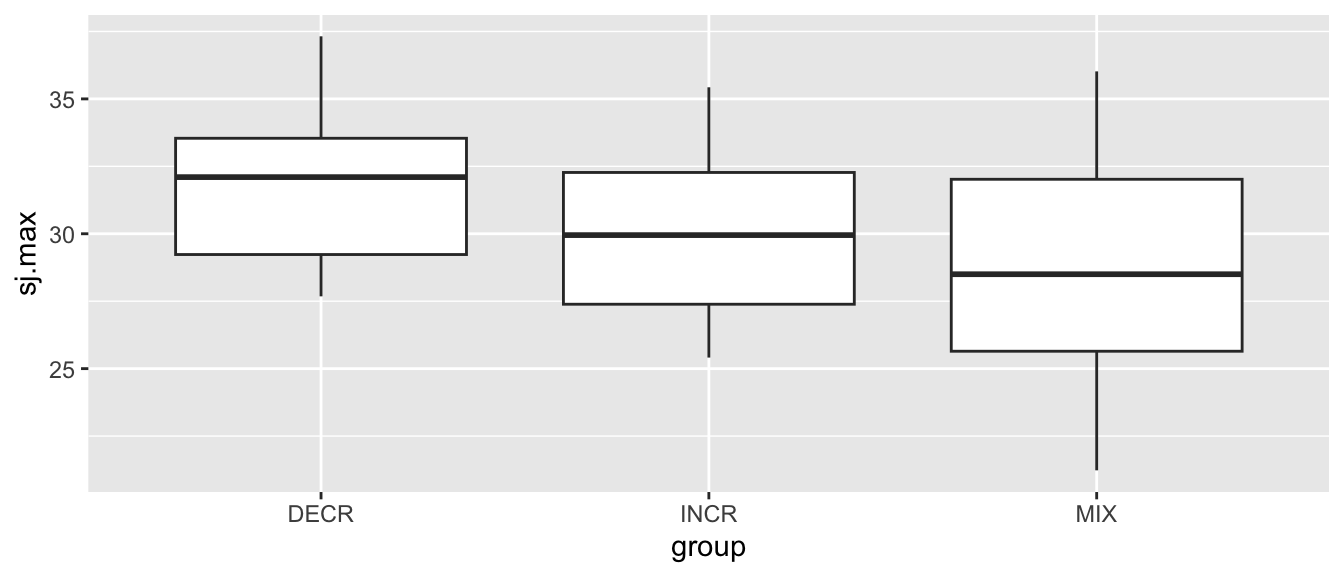
\includegraphics{04-first-graph_files/figure-pdf/fig-boxplot-simple-1.pdf}

}

\caption{\label{fig-boxplot-simple}Boxplot of all data per group from
the cycling dataset.}

\end{figure}

We can add layers of more geoms to the same plot. We might want to add
individual data points also. \texttt{geom\_jitter} might be a good place
to start. This geom is good as it can be plotted over a group variable
and points gets ``jittered'' or spread so we avoid overlap.

\begin{Shaded}
\begin{Highlighting}[numbers=left,,]
\CommentTok{\# Creating a boxplot of all values per group}
\FunctionTok{ggplot}\NormalTok{(cycdat, }\FunctionTok{aes}\NormalTok{(group, sj.max)) }\SpecialCharTok{+} \FunctionTok{geom\_boxplot}\NormalTok{() }\SpecialCharTok{+} \FunctionTok{geom\_jitter}\NormalTok{()}
\end{Highlighting}
\end{Shaded}

\begin{verbatim}
Warning: Removed 4 rows containing non-finite values (`stat_boxplot()`).
\end{verbatim}

\begin{verbatim}
Warning: Removed 4 rows containing missing values (`geom_point()`).
\end{verbatim}

\begin{figure}[H]

{\centering 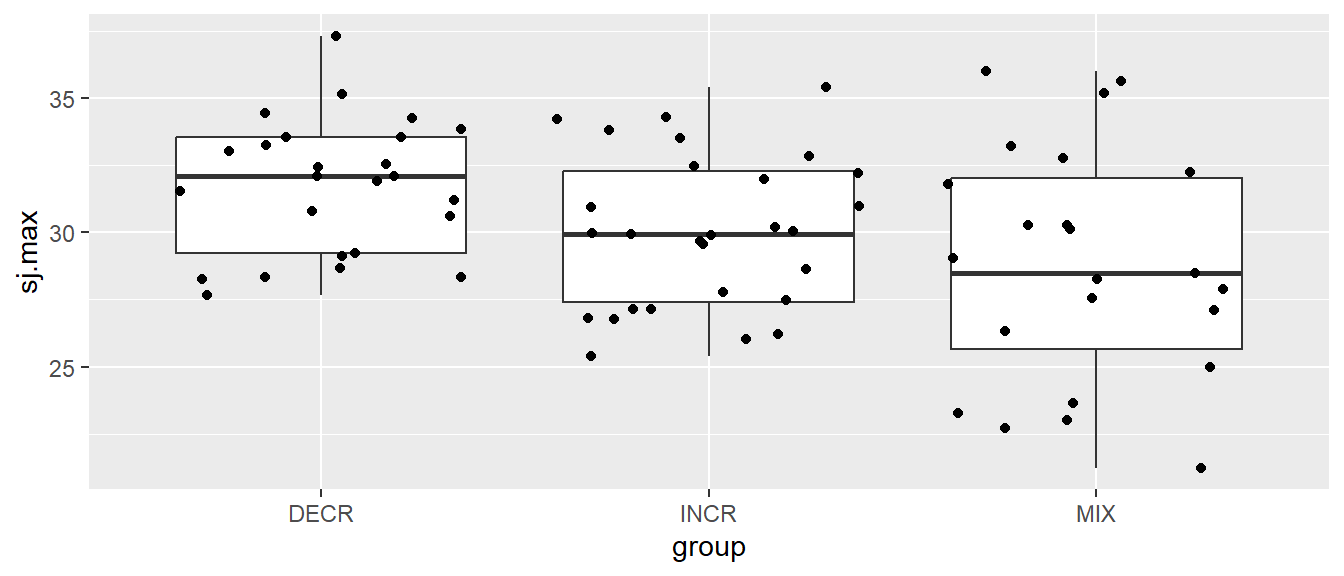
\includegraphics{04-first-graph_files/figure-pdf/fig-boxplot-jitter-1.pdf}

}

\caption{\label{fig-boxplot-jitter}Box-plot and jittered points of all
data per group from the cycling dataset.}

\end{figure}

Notice that we get warnings saying that there are some data missing,
these values are removed from the calculation of summary statistics in
the box-plots and omitted from plotting of the points.

\hypertarget{data-over-time-per-group-and-individual}{%
\subsection{Data over time per group and
individual}\label{data-over-time-per-group-and-individual}}

In the data set we have a time variable consisting of the labels
``pre'', ``meso1'', ``meso2'' and ``meso3''. When we load the data into
R we do so without providing information about the order of these
labels. R will put them in alphabetical order when order is required (as
in a figure). If we want to plot these data in the right order, we have
to tell R that these data should have an order. We will convert the
\texttt{timepoint} variable to a factor. Factors are variables that can
contain more information than what is contained in each cell. Using the
\texttt{factor} function we will set the order of the \texttt{timepoint}
variable. We assign this transformation of the variable to its original
place in the data frame.

\begin{Shaded}
\begin{Highlighting}[numbers=left,,]
\NormalTok{cycdat}\SpecialCharTok{$}\NormalTok{timepoint }\OtherTok{\textless{}{-}} \FunctionTok{factor}\NormalTok{(cycdat}\SpecialCharTok{$}\NormalTok{timepoint, }\AttributeTok{levels =} \FunctionTok{c}\NormalTok{(}\StringTok{"pre"}\NormalTok{, }\StringTok{"meso1"}\NormalTok{, }\StringTok{"meso2"}\NormalTok{, }\StringTok{"meso3"}\NormalTok{))}
\end{Highlighting}
\end{Shaded}

We are now ready to plot data over time, where the time variable is
correctly ordered. Let's use the box-plot again to plot all values over
time.

\begin{Shaded}
\begin{Highlighting}[numbers=left,,]
\CommentTok{\# Creating a boxplot of all values per time point}
\FunctionTok{ggplot}\NormalTok{(cycdat, }\FunctionTok{aes}\NormalTok{(timepoint, sj.max)) }\SpecialCharTok{+} \FunctionTok{geom\_boxplot}\NormalTok{()}
\end{Highlighting}
\end{Shaded}

\begin{verbatim}
Warning: Removed 4 rows containing non-finite values (`stat_boxplot()`).
\end{verbatim}

\begin{figure}[H]

{\centering 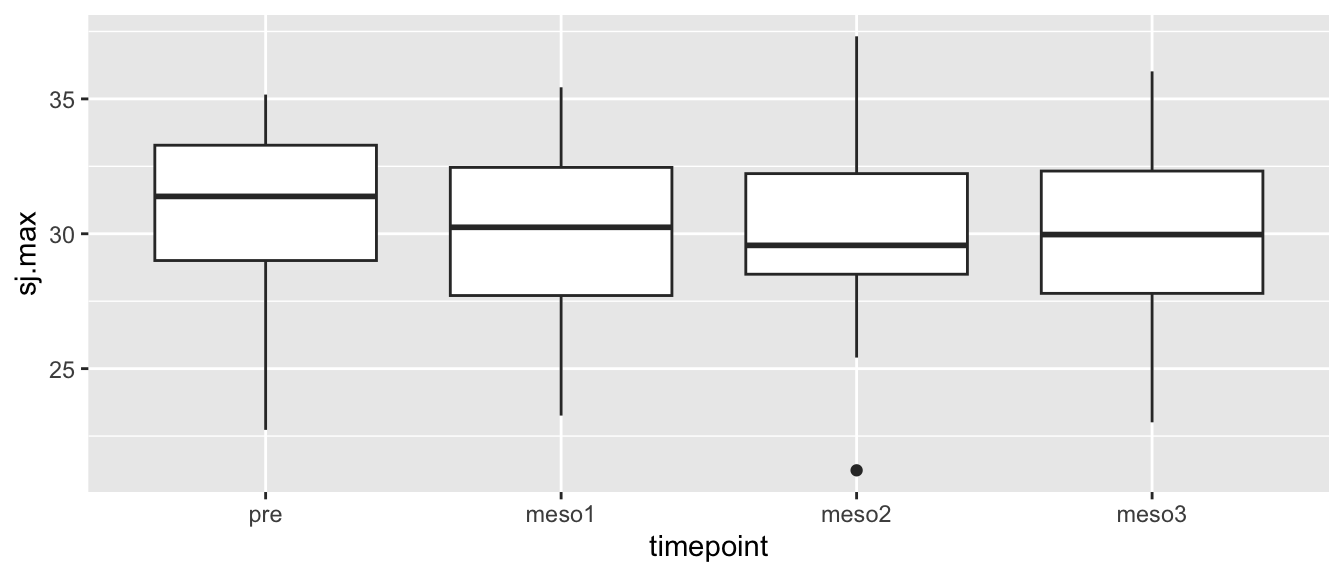
\includegraphics{04-first-graph_files/figure-pdf/fig-boxplot-time-1.pdf}

}

\caption{\label{fig-boxplot-time}Boxplot of all data per time-point from
the cycling dataset.}

\end{figure}

We do not see any great tendencies in the whole data set. To further
explore the data we might want to have different boxes per group per
time. We can accomplish this by adding \texttt{fill\ =\ group} to our
\texttt{aes} function.

\begin{Shaded}
\begin{Highlighting}[numbers=left,,]
\CommentTok{\# Creating a boxplot of all values per group over time}
\FunctionTok{ggplot}\NormalTok{(cycdat, }\FunctionTok{aes}\NormalTok{(timepoint, sj.max, }\AttributeTok{fill =}\NormalTok{ group)) }\SpecialCharTok{+} \FunctionTok{geom\_boxplot}\NormalTok{()}
\end{Highlighting}
\end{Shaded}

\begin{verbatim}
Warning: Removed 4 rows containing non-finite values (`stat_boxplot()`).
\end{verbatim}

\begin{figure}[H]

{\centering 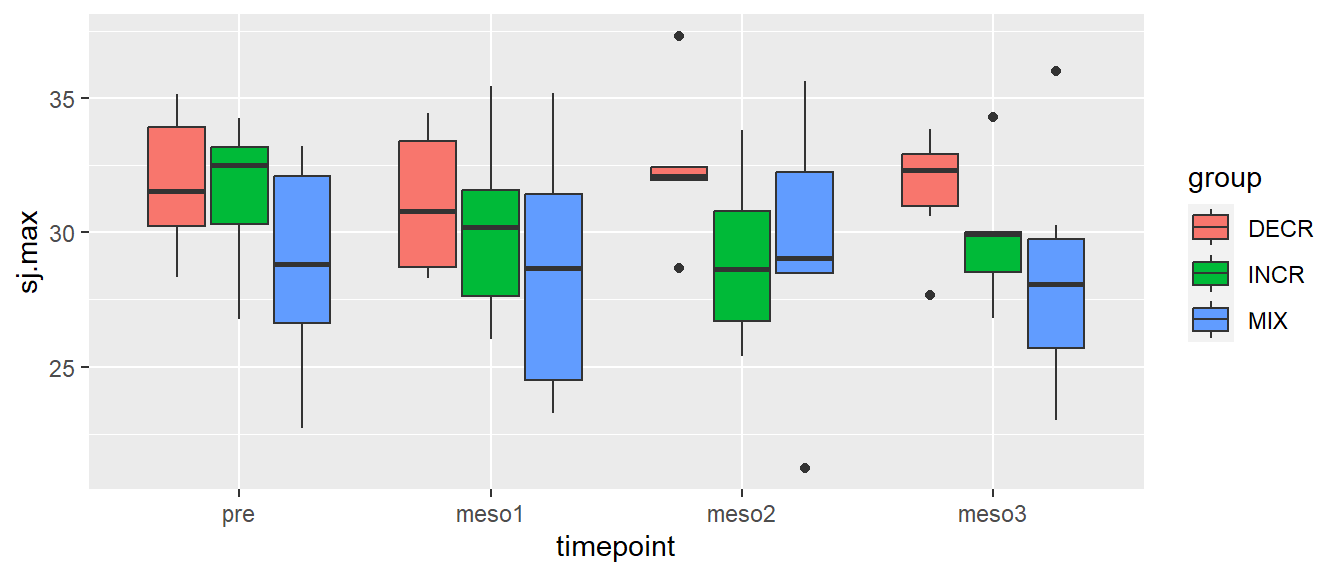
\includegraphics{04-first-graph_files/figure-pdf/fig-boxplot-time-fill-1.pdf}

}

\caption{\label{fig-boxplot-time-fill}Boxplot of all data per time-point
and group from the cycling dataset.}

\end{figure}

This is possible because \texttt{geom\_boxplots} can be filled. The same
separation of groups would have been accomplished using
\texttt{color\ =\ group}, however, then the boxes would get different
border colors instead. You might have noticed that the box-plots do not
contain all the data, a few data points are outside \(1.5 \times IQR\)
(interquartile range). This, by standard definitions, defines the data
point as an ``outlier''.

As mentioned above, box-plots does some summarizing and not all data is
shown. To explore further we might want to track every participant. To
do this we have to tell \texttt{ggplot} how to group the data. In
\texttt{aes()} the group argument let's you connect lines based on some
grouping variable, in our case it will be \texttt{subject}. We will use
a line to connect each participants score over time. Using
\texttt{color\ =\ group} will additionally give every line a different
color depending on which group it belongs to.

\begin{Shaded}
\begin{Highlighting}[numbers=left,,]
\CommentTok{\# Creating a line plot of all values per participant over time, color per group}

\FunctionTok{ggplot}\NormalTok{(cycdat, }\FunctionTok{aes}\NormalTok{(timepoint, sj.max, }\AttributeTok{color =}\NormalTok{ group, }\AttributeTok{group =}\NormalTok{ subject)) }\SpecialCharTok{+} 
\FunctionTok{geom\_line}\NormalTok{()}
\end{Highlighting}
\end{Shaded}

\begin{verbatim}
Warning: Removed 2 rows containing missing values (`geom_line()`).
\end{verbatim}

\begin{figure}[H]

{\centering 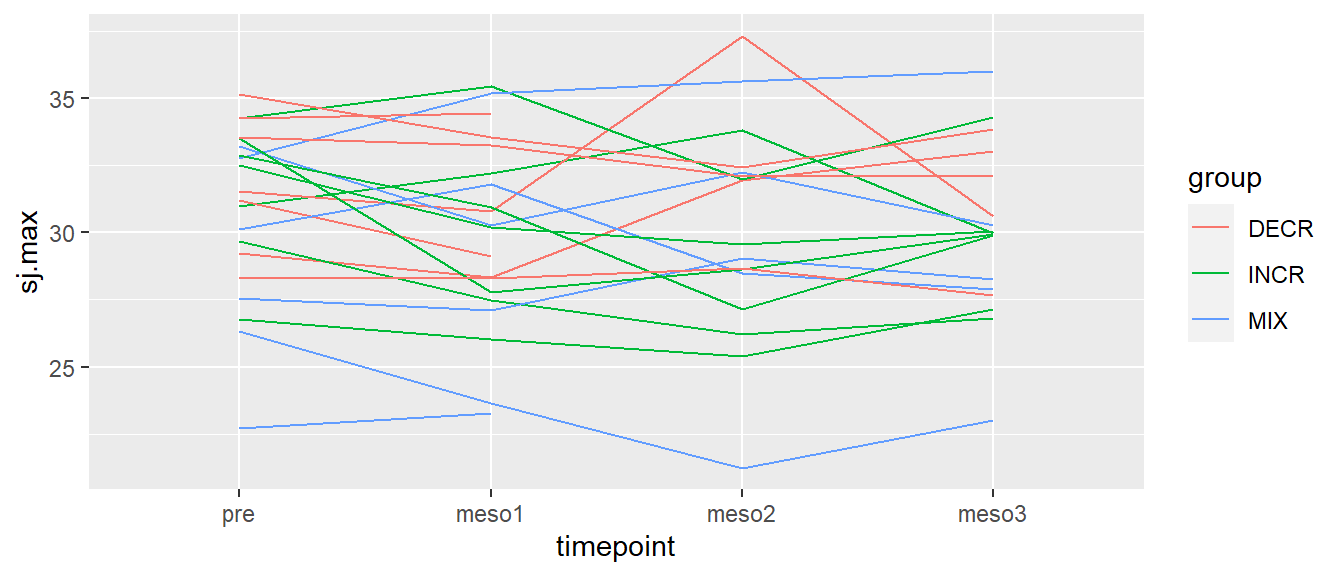
\includegraphics{04-first-graph_files/figure-pdf/fig-sj-ind-data-1.pdf}

}

\caption{\label{fig-sj-ind-data}Figure with lines corresponding to
indivudal values per participant.}

\end{figure}

In Figure~\ref{fig-sj-ind-data}, each line represents a participant,
different colors represents different groups.

\hypertarget{titles-and-labels}{%
\subsection{Titles and labels}\label{titles-and-labels}}

Often we need to add information to the plot to better communicate its
message. Such information could be appropriate titles on axes and
legends and extra text needed to explain aspects of the plot. Using the
\texttt{labs()} function we can add information that will replace
variable names that are being used for all variables that have been
mapped in the figure. In the figure below we will start by adding better
axis titles. This information goes into \texttt{x} and \texttt{y} in
\texttt{labs()} which simply changes the titles of the x- and y-axis.

\begin{Shaded}
\begin{Highlighting}[numbers=left,,]
\CommentTok{\# Creating a line plot of all values per participant over time, color per group, }
\CommentTok{\# adding axis labels}
\FunctionTok{ggplot}\NormalTok{(cycdat, }\FunctionTok{aes}\NormalTok{(timepoint, sj.max, }\AttributeTok{color =}\NormalTok{ group, }\AttributeTok{group =}\NormalTok{ subject)) }\SpecialCharTok{+} 
  \FunctionTok{geom\_line}\NormalTok{() }\SpecialCharTok{+}
  \FunctionTok{labs}\NormalTok{(}\AttributeTok{x =} \StringTok{"Time{-}point"}\NormalTok{,}
       \AttributeTok{y =} \StringTok{"Squat jump height (cm)"}\NormalTok{)}
\end{Highlighting}
\end{Shaded}

\begin{verbatim}
Warning: Removed 2 rows containing missing values (`geom_line()`).
\end{verbatim}

\begin{figure}[H]

{\centering 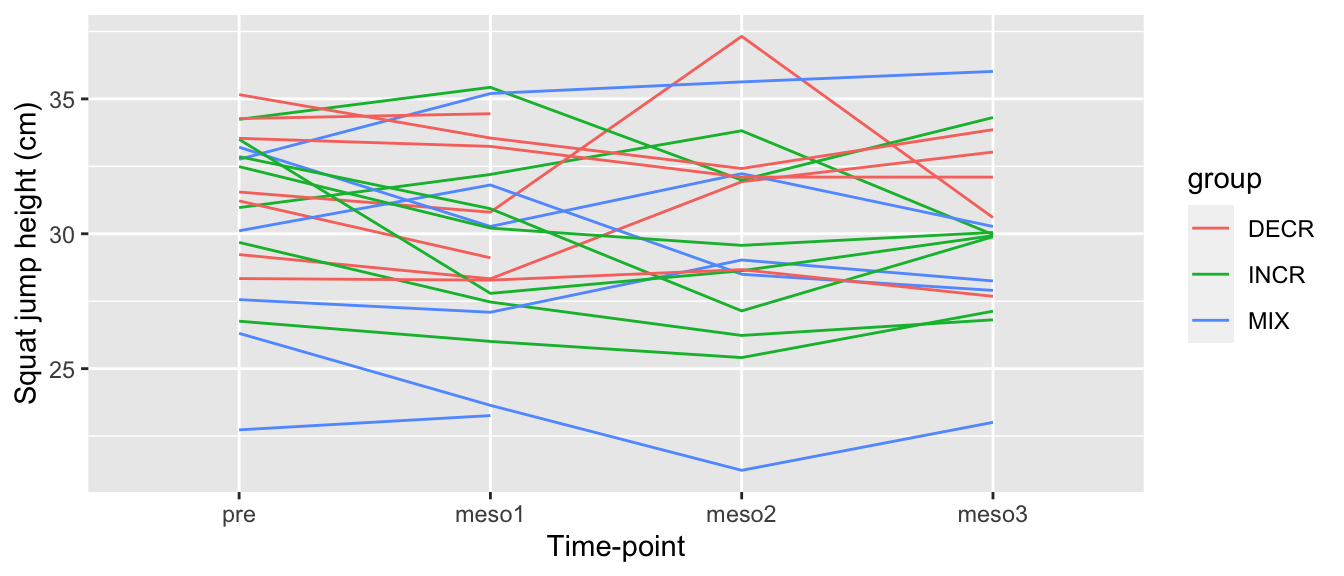
\includegraphics{04-first-graph_files/figure-pdf/fig-ind-data-axis-title-1.pdf}

}

\caption{\label{fig-ind-data-axis-title}Figure with updated axis labels}

\end{figure}

The resulting Figure~\ref{fig-ind-data-axis-title} now have better
titles for each axis. Notice in the code above that titles needs to be
specified with quotation marks. This is a tricky aspect of R, if we
would have omitted the quotation marks we would have told R to look for
objects by the name of e.g.~\texttt{Time-point}, and this would actually
mean that we tried to subtract \texttt{time} from \texttt{point} since
\texttt{-} is interpreted as a minus sign.

We might want to add information to the legend also. Since we specified
\texttt{color\ =\ group} in the \texttt{aes()} function, the same can be
manipulated in \texttt{labs}. Lets just add a capital G.

\begin{Shaded}
\begin{Highlighting}[numbers=left,,]
\FunctionTok{ggplot}\NormalTok{(cycdat, }\FunctionTok{aes}\NormalTok{(timepoint, sj.max, }\AttributeTok{color =}\NormalTok{ group, }\AttributeTok{group =}\NormalTok{ subject)) }\SpecialCharTok{+} 
  \FunctionTok{geom\_line}\NormalTok{() }\SpecialCharTok{+}
  \FunctionTok{labs}\NormalTok{(}\AttributeTok{x =} \StringTok{"Time{-}point"}\NormalTok{,}
       \AttributeTok{y =} \StringTok{"Squat jump height (cm)"}\NormalTok{, }
       \AttributeTok{color =} \StringTok{"Group"}\NormalTok{)}
\end{Highlighting}
\end{Shaded}

\begin{verbatim}
Warning: Removed 2 rows containing missing values (`geom_line()`).
\end{verbatim}

\begin{figure}[H]

{\centering 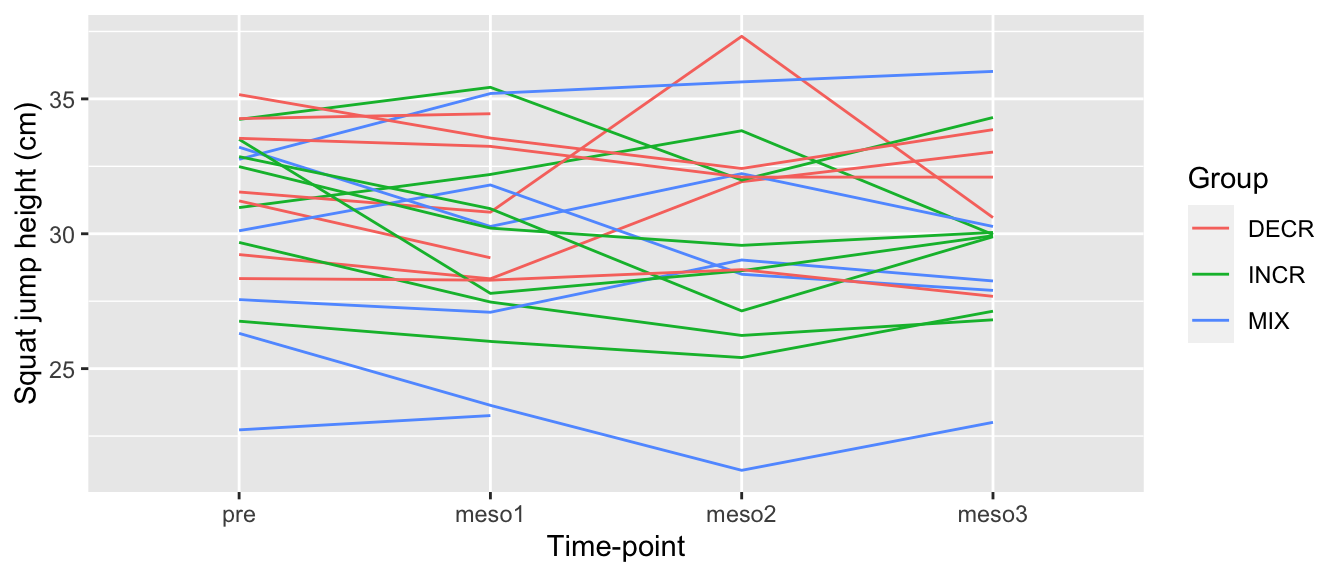
\includegraphics{04-first-graph_files/figure-pdf/fig-ind-data-axis-color-title-1.pdf}

}

\caption{\label{fig-ind-data-axis-color-title}Additional labels}

\end{figure}

We still have the original labels for the time variable. Remember that
we used the \texttt{factor} function above to set the order of the
labels. Actually we specified the ``levels'' of the factor. We can use
the same function to add better ``labels''. In the code below, I will
first change the variable in the data set and then use the exact same
code for the plot.

\begin{Shaded}
\begin{Highlighting}[numbers=left,,]
\NormalTok{cycdat}\SpecialCharTok{$}\NormalTok{timepoint }\OtherTok{\textless{}{-}} \FunctionTok{factor}\NormalTok{(cycdat}\SpecialCharTok{$}\NormalTok{timepoint, }\AttributeTok{levels =} \FunctionTok{c}\NormalTok{(}\StringTok{"pre"}\NormalTok{, }\StringTok{"meso1"}\NormalTok{, }\StringTok{"meso2"}\NormalTok{, }\StringTok{"meso3"}\NormalTok{), }
                           \AttributeTok{labels =} \FunctionTok{c}\NormalTok{(}\StringTok{"Pre{-}training"}\NormalTok{, }\StringTok{"Meso{-}cycle 1"}\NormalTok{, }\StringTok{"Meso{-}cycle 2"}\NormalTok{, }\StringTok{"Meso{-}cycle 3"}\NormalTok{))}

\FunctionTok{ggplot}\NormalTok{(cycdat, }\FunctionTok{aes}\NormalTok{(timepoint, sj.max, }\AttributeTok{color =}\NormalTok{ group, }\AttributeTok{group =}\NormalTok{ subject)) }\SpecialCharTok{+} 
  \FunctionTok{geom\_line}\NormalTok{() }\SpecialCharTok{+}
  \FunctionTok{labs}\NormalTok{(}\AttributeTok{x =} \StringTok{"Time{-}point"}\NormalTok{,}
       \AttributeTok{y =} \StringTok{"Squat jump height (cm)"}\NormalTok{, }
       \AttributeTok{color =} \StringTok{"Group"}\NormalTok{)}
\end{Highlighting}
\end{Shaded}

\begin{verbatim}
Warning: Removed 2 rows containing missing values (`geom_line()`).
\end{verbatim}

\begin{figure}[H]

{\centering 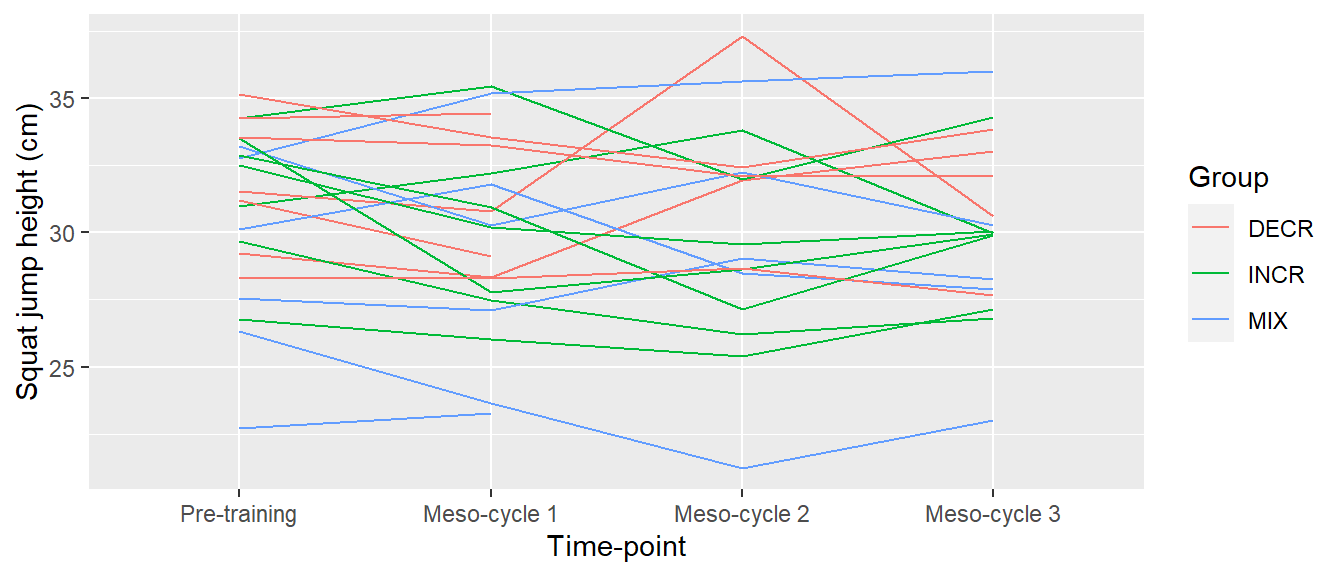
\includegraphics{04-first-graph_files/figure-pdf/fig-factor-labels-1.pdf}

}

\caption{\label{fig-factor-labels}Changing labels by changing a factor
variable prior to plotting}

\end{figure}

The same goes for the group variable. You can try to change the levels
and labels of the grouping variable to make it more descriptive. You can
type \texttt{?cyclingstudy} in your console to read about the group
variable and then use this information to write better labels using the
\texttt{factor} function. In the factor function, the first argument is
the variable you want to use as basis of your new factor, the second
argument you need to specify is \texttt{levels} which sets the order and
lastly you will need to set the labels for each level using
\texttt{labels\ =}. If you write \texttt{?factor} in your console you
will get the help pages for the \texttt{factor} function.

Click here to display a possible solution

\hypertarget{toggleText1}{}
\begin{Shaded}
\begin{Highlighting}[numbers=left,,]
\CommentTok{\# Change the grouping variable}
\NormalTok{cycdat}\SpecialCharTok{$}\NormalTok{group }\OtherTok{\textless{}{-}} \FunctionTok{factor}\NormalTok{(cycdat}\SpecialCharTok{$}\NormalTok{group, }\AttributeTok{levels =} \FunctionTok{c}\NormalTok{(}\StringTok{"DECR"}\NormalTok{, }\StringTok{"INCR"}\NormalTok{, }\StringTok{"MIX"}\NormalTok{), }
                           \AttributeTok{labels =} \FunctionTok{c}\NormalTok{(}\StringTok{"Decreased}\SpecialCharTok{\textbackslash{}n}\StringTok{intensity"}\NormalTok{, }
                                      \StringTok{"Increased}\SpecialCharTok{\textbackslash{}n}\StringTok{intensity"}\NormalTok{, }
                                      \StringTok{"Mixed}\SpecialCharTok{\textbackslash{}n}\StringTok{intensity"}\NormalTok{))}

\CommentTok{\# Plotting the data as before with the new information added}
\FunctionTok{ggplot}\NormalTok{(cycdat, }\FunctionTok{aes}\NormalTok{(timepoint, sj.max, }\AttributeTok{color =}\NormalTok{ group, }\AttributeTok{group =}\NormalTok{ subject)) }\SpecialCharTok{+} 
  \FunctionTok{geom\_line}\NormalTok{() }\SpecialCharTok{+}
  \FunctionTok{labs}\NormalTok{(}\AttributeTok{x =} \StringTok{"Time{-}point"}\NormalTok{,}
       \AttributeTok{y =} \StringTok{"Squat jump height (cm)"}\NormalTok{, }
       \AttributeTok{color =} \StringTok{"Periodization strategy"}\NormalTok{)}
\end{Highlighting}
\end{Shaded}

Note: Adding \texttt{\textbackslash{}n} in the the text string breaks
the line to get two rows.

\hypertarget{annotations}{%
\subsection{Annotations}\label{annotations}}

Annotation may become handy when you want to add elements to the graph
that is not in the data set. Using ggplot2, annotations are added using
the \texttt{annotate()} function. This function first needs to be
specified with a geom, these are commonly text or lines or segments. In
the code chunk below are several examples of annotations. First I save
the plot as an object called \texttt{myplot} and then add different
annotations to it.

\begin{Shaded}
\begin{Highlighting}[numbers=left,,]
\NormalTok{myplot }\OtherTok{\textless{}{-}} \FunctionTok{ggplot}\NormalTok{(cycdat, }\FunctionTok{aes}\NormalTok{(timepoint, sj.max, }\AttributeTok{color =}\NormalTok{ group, }\AttributeTok{group =}\NormalTok{ subject)) }\SpecialCharTok{+} 
  \FunctionTok{geom\_line}\NormalTok{() }\SpecialCharTok{+}
  \FunctionTok{labs}\NormalTok{(}\AttributeTok{x =} \StringTok{"Time{-}point"}\NormalTok{,}
       \AttributeTok{y =} \StringTok{"Squat jump height (cm)"}\NormalTok{, }
       \AttributeTok{color =} \StringTok{"Periodization strategy"}\NormalTok{) }


\CommentTok{\# A text annotation}
\NormalTok{myplot }\SpecialCharTok{+} \FunctionTok{annotate}\NormalTok{(}\StringTok{"text"}\NormalTok{, }\AttributeTok{x =} \DecValTok{1}\NormalTok{, }\AttributeTok{y =} \DecValTok{37}\NormalTok{, }\AttributeTok{label =} \StringTok{"This is an annotation"}\NormalTok{)}

\CommentTok{\# A line/segment }
\NormalTok{myplot }\SpecialCharTok{+} \FunctionTok{annotate}\NormalTok{(}\StringTok{"segment"}\NormalTok{, }\AttributeTok{x =} \DecValTok{1}\NormalTok{, }\AttributeTok{xend =} \DecValTok{3}\NormalTok{, }\AttributeTok{y =} \DecValTok{25}\NormalTok{, }\AttributeTok{yend =} \DecValTok{35}\NormalTok{,  }\AttributeTok{colour =} \StringTok{"red"}\NormalTok{, }\AttributeTok{size =} \DecValTok{4}\NormalTok{)}
\end{Highlighting}
\end{Shaded}

You can copy the code and run it yourself to see the results.
\texttt{annotate} is documented
\href{https://ggplot2.tidyverse.org/reference/annotate.html}{here} but
documentation can also be accessed by typing \texttt{?annotate} in your
console. Try to read the documentation and add a transparent rectangle
to a previous plot.

Click here for a solution

\hypertarget{toggleText2}{}
\begin{Shaded}
\begin{Highlighting}[numbers=left,,]
\CommentTok{\# Change the grouping variable}
\NormalTok{cycdat}\SpecialCharTok{$}\NormalTok{group }\OtherTok{\textless{}{-}} \FunctionTok{factor}\NormalTok{(cycdat}\SpecialCharTok{$}\NormalTok{group, }\AttributeTok{levels =} \FunctionTok{c}\NormalTok{(}\StringTok{"DECR"}\NormalTok{, }\StringTok{"INCR"}\NormalTok{, }\StringTok{"MIX"}\NormalTok{), }
                           \AttributeTok{labels =} \FunctionTok{c}\NormalTok{(}\StringTok{"Decreased}\SpecialCharTok{\textbackslash{}n}\StringTok{intensity"}\NormalTok{, }
                                      \StringTok{"Increased}\SpecialCharTok{\textbackslash{}n}\StringTok{intensity"}\NormalTok{, }
                                      \StringTok{"Mixed}\SpecialCharTok{\textbackslash{}n}\StringTok{intensity"}\NormalTok{))}

\CommentTok{\# Plotting the data as before with the new information added}
\FunctionTok{ggplot}\NormalTok{(cycdat, }\FunctionTok{aes}\NormalTok{(timepoint, sj.max, }\AttributeTok{color =}\NormalTok{ group, }\AttributeTok{group =}\NormalTok{ subject)) }\SpecialCharTok{+} 
  \FunctionTok{geom\_line}\NormalTok{() }\SpecialCharTok{+}
  \FunctionTok{labs}\NormalTok{(}\AttributeTok{x =} \StringTok{"Time{-}point"}\NormalTok{,}
       \AttributeTok{y =} \StringTok{"Squat jump height (cm)"}\NormalTok{, }
       \AttributeTok{color =} \StringTok{"Periodization strategy"}\NormalTok{) }\SpecialCharTok{+}
  \CommentTok{\# A rectangular annotation (alpha = 0.4 makes the rectangle transparent)}
 \FunctionTok{annotate}\NormalTok{(}\StringTok{"rect"}\NormalTok{, }\AttributeTok{xmin =} \DecValTok{1}\NormalTok{, }\AttributeTok{xmax =} \DecValTok{2}\NormalTok{, }\AttributeTok{ymin =} \DecValTok{30}\NormalTok{, }\AttributeTok{ymax =} \DecValTok{35}\NormalTok{, }\AttributeTok{alpha =} \FloatTok{0.4}\NormalTok{)}
\end{Highlighting}
\end{Shaded}

Note: Adding \texttt{\textbackslash{}n} in the the text string breaks
the line to get two rows.

\hypertarget{themes}{%
\section{Themes}\label{themes}}

Themes in \texttt{ggplot2} can be used to change everything else about
the plot concerning text, colors etc. \texttt{ggplot2} has some built in
themes that are easily activated by adding them to the plot. For example
the \texttt{theme\_bw()} function will change the theme to a black and
white one as in the figure below.

\begin{Shaded}
\begin{Highlighting}[numbers=left,,]
\FunctionTok{ggplot}\NormalTok{(cycdat, }\FunctionTok{aes}\NormalTok{(timepoint, sj.max, }\AttributeTok{color =}\NormalTok{ group, }\AttributeTok{group =}\NormalTok{ subject)) }\SpecialCharTok{+} 
  \FunctionTok{geom\_line}\NormalTok{() }\SpecialCharTok{+}
  \FunctionTok{labs}\NormalTok{(}\AttributeTok{x =} \StringTok{"Time{-}point"}\NormalTok{,}
       \AttributeTok{y =} \StringTok{"Squat jump height (cm)"}\NormalTok{, }
       \AttributeTok{color =} \StringTok{"Group"}\NormalTok{) }\SpecialCharTok{+} 
  \FunctionTok{theme\_bw}\NormalTok{() }\CommentTok{\# Adding a pre{-}specified theme}
\end{Highlighting}
\end{Shaded}

\begin{verbatim}
Warning: Removed 2 rows containing missing values (`geom_line()`).
\end{verbatim}

\begin{figure}[H]

{\centering 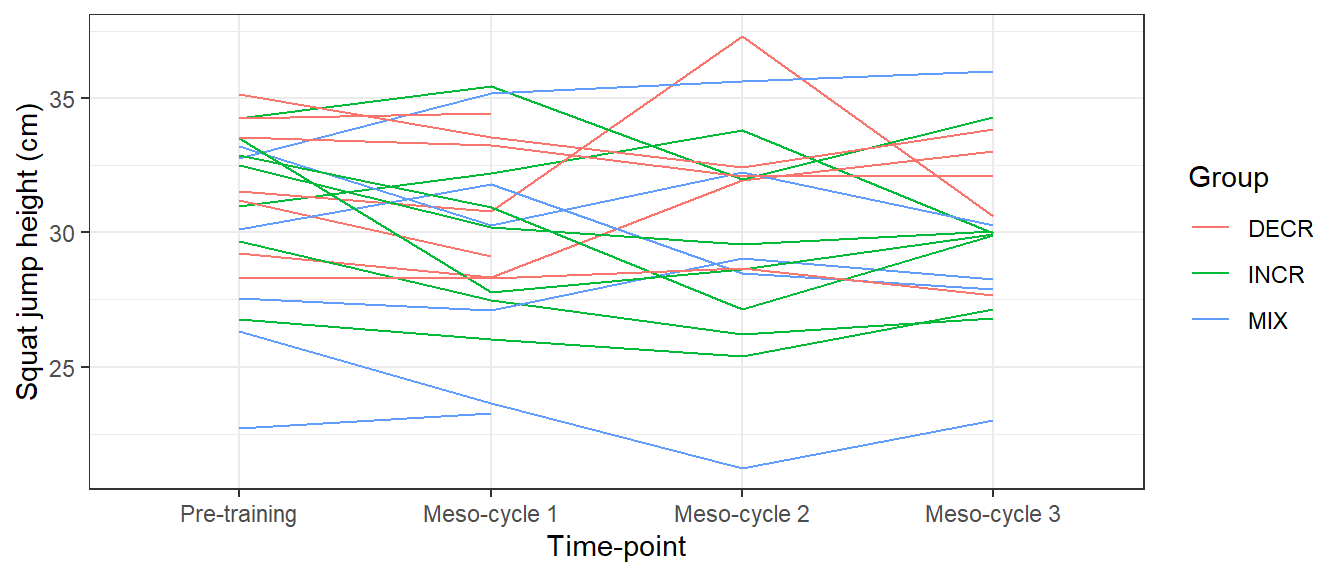
\includegraphics{04-first-graph_files/figure-pdf/fig-theme-bw-1.pdf}

}

\caption{\label{fig-theme-bw}A figure using the black and white theme
from \texttt{theme\_bw}.}

\end{figure}

A collection of built in themes are documented
\href{https://ggplot2.tidyverse.org/reference/ggtheme.html}{here}.
Individual components of the theme can also be changed using the
\texttt{theme()} function. There is a long list of theme components that
can be changed using this function. The list can be found
\href{https://ggplot2.tidyverse.org/reference/theme.html}{here}.\\
If we put the \texttt{theme} function last in the \texttt{ggplot} call
we will modify the existing theme. Let's say that we want to change the
color of the text on the x axis.

\begin{Shaded}
\begin{Highlighting}[numbers=left,,]
\FunctionTok{ggplot}\NormalTok{(cycdat, }\FunctionTok{aes}\NormalTok{(timepoint, sj.max, }\AttributeTok{color =}\NormalTok{ group, }\AttributeTok{group =}\NormalTok{ subject)) }\SpecialCharTok{+} 
  \FunctionTok{geom\_line}\NormalTok{() }\SpecialCharTok{+}
  \FunctionTok{labs}\NormalTok{(}\AttributeTok{x =} \StringTok{"Time{-}point"}\NormalTok{,}
       \AttributeTok{y =} \StringTok{"Squat jump height (cm)"}\NormalTok{, }
       \AttributeTok{color =} \StringTok{"Group"}\NormalTok{) }\SpecialCharTok{+} 
  \FunctionTok{theme\_bw}\NormalTok{() }\SpecialCharTok{+}
  \FunctionTok{theme}\NormalTok{(}\AttributeTok{axis.text.x =} \FunctionTok{element\_text}\NormalTok{(}\AttributeTok{color =} \StringTok{"steelblue"}\NormalTok{, }\AttributeTok{size =} \DecValTok{12}\NormalTok{, }\AttributeTok{face =} \StringTok{"bold"}\NormalTok{))}
\end{Highlighting}
\end{Shaded}

\begin{verbatim}
Warning: Removed 2 rows containing missing values (`geom_line()`).
\end{verbatim}

\begin{figure}[H]

{\centering 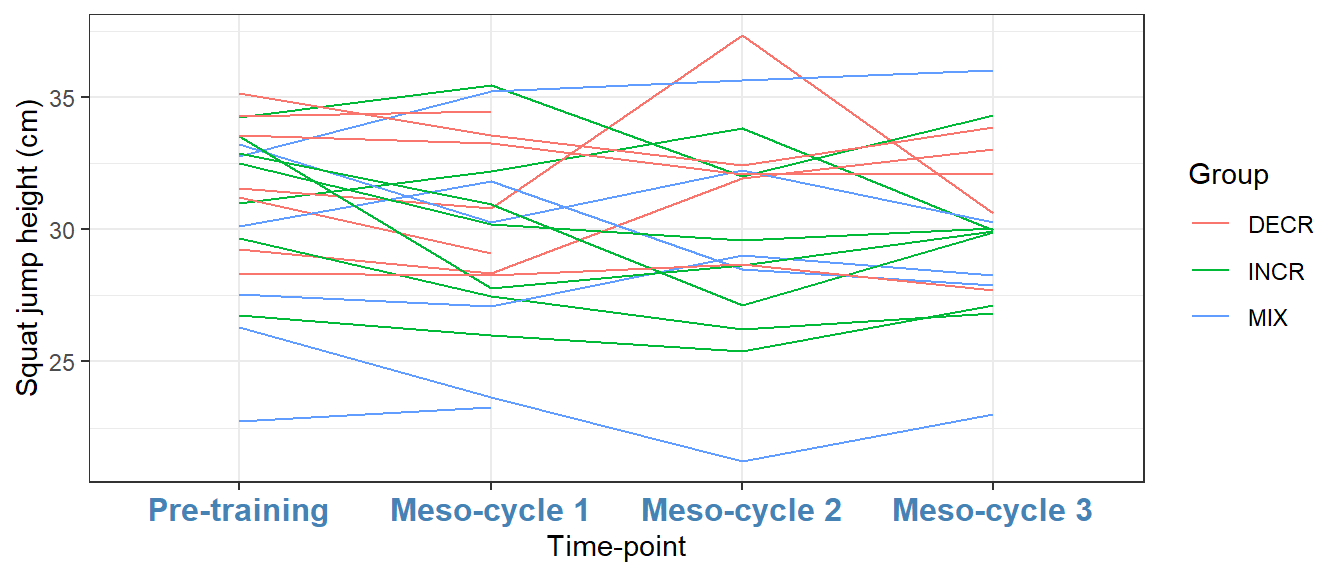
\includegraphics{04-first-graph_files/figure-pdf/fig-theme-bw-changed-1.pdf}

}

\caption{\label{fig-theme-bw-changed}A figure using the black and white
theme from \texttt{theme\_bw}, with modifications}

\end{figure}

The component \texttt{axis.text.x} can be modified using a function that
changes appearance of text components, namely \texttt{element\_text}.
Similarly, other components are changed with specific functions for
lines and rectangular shapes (see the help pages for \texttt{theme}).

\hypertarget{test-your-understandning}{%
\section{Test your understandning}\label{test-your-understandning}}

In this section you can try to implement what we have discussed above.
An example solution exists below each figure by press of button.

In Figure~\ref{fig-example-1}, I have used the VO2max data from the
\texttt{cyclingstudy} data set. I have made changes to the time variable
(\texttt{timepoint}) to make the labels better. I have added a title to
the figure and changed the appearance of the text. I will use an extra
package called (ggtext){[}https://wilkelab.org/ggtext/index.html{]} to
make it possible to use markdown syntax in axis labels. In order to use
\texttt{ggtext} you have to install it from CRAN.

\begin{figure}

{\centering 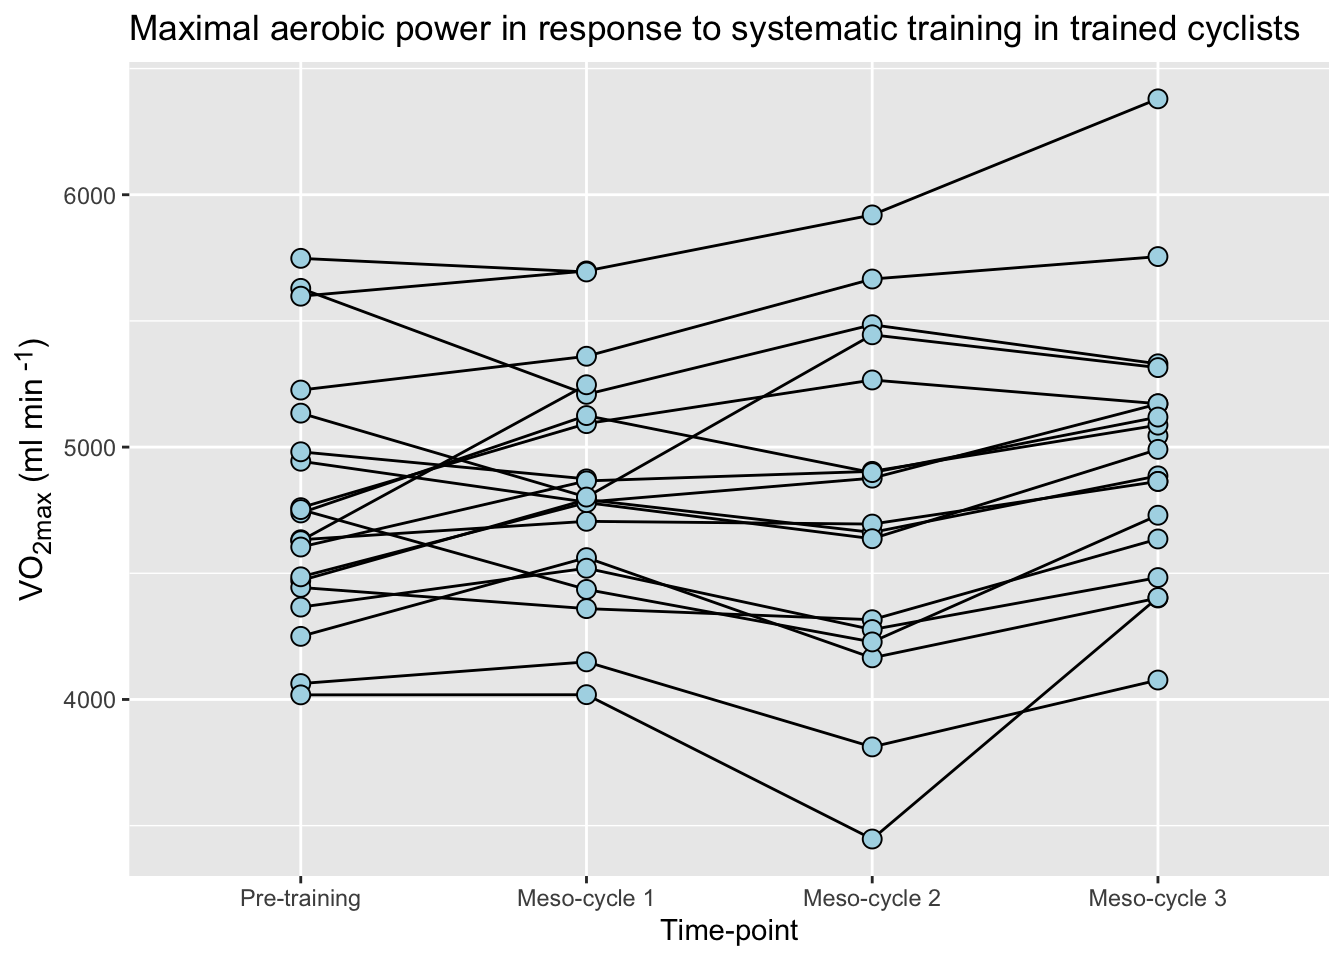
\includegraphics{04-first-graph_files/figure-pdf/fig-example-1-1.pdf}

}

\caption{\label{fig-example-1}Example figure 1}

\end{figure}

Click for a solution

\hypertarget{toggleText3}{}
\begin{Shaded}
\begin{Highlighting}[numbers=left,,]
\CommentTok{\# Load the package ggtext to make markdown avalable in axis labels.}
\FunctionTok{library}\NormalTok{(ggtext) }

\CommentTok{\# For ease of use I save a smaller dataset in a new object}
\NormalTok{cycdat }\OtherTok{\textless{}{-}} \FunctionTok{select}\NormalTok{(cyclingstudy, subject, timepoint, VO2.max)}

\CommentTok{\# Change the labels of the time variable}
\NormalTok{cycdat}\SpecialCharTok{$}\NormalTok{timepoint }\OtherTok{\textless{}{-}} \FunctionTok{factor}\NormalTok{(cycdat}\SpecialCharTok{$}\NormalTok{timepoint, }\AttributeTok{levels =} \FunctionTok{c}\NormalTok{(}\StringTok{"pre"}\NormalTok{, }\StringTok{"meso1"}\NormalTok{, }\StringTok{"meso2"}\NormalTok{, }\StringTok{"meso3"}\NormalTok{), }
                           \AttributeTok{labels =} \FunctionTok{c}\NormalTok{(}\StringTok{"Pre{-}training"}\NormalTok{, }\StringTok{"Meso{-}cycle 1"}\NormalTok{, }\StringTok{"Meso{-}cycle 2"}\NormalTok{, }\StringTok{"Meso{-}cycle 3"}\NormalTok{))}


\CommentTok{\# create the basic plot}

\FunctionTok{ggplot}\NormalTok{(}\AttributeTok{data =}\NormalTok{ cycdat, }\FunctionTok{aes}\NormalTok{(timepoint, VO2.max, }\AttributeTok{group =}\NormalTok{ subject)) }\SpecialCharTok{+} 
  \CommentTok{\# Add lines to connect dots. Putting the lines first and plotting points on top}
  \FunctionTok{geom\_line}\NormalTok{() }\SpecialCharTok{+} 
  \CommentTok{\# Add points foe each participant/time}
  \FunctionTok{geom\_point}\NormalTok{(}\AttributeTok{size =} \DecValTok{3}\NormalTok{, }\AttributeTok{fill =} \StringTok{"lightblue"}\NormalTok{, }\AttributeTok{shape =} \DecValTok{21}\NormalTok{) }\SpecialCharTok{+} 

  \CommentTok{\# Adding correct axis titles and a figure title}
  \FunctionTok{labs}\NormalTok{(}\AttributeTok{x =} \StringTok{"Time{-}point"}\NormalTok{, }
       \AttributeTok{y =} \StringTok{"VO\textless{}sub\textgreater{}2max\textless{}/sub\textgreater{} (ml min\textless{}sup\textgreater{} {-}1\textless{}/sup\textgreater{})"}\NormalTok{, }
       \AttributeTok{title =} \StringTok{"Maximal aerobic power in response to systematic training in trained cyclists"}\NormalTok{) }\SpecialCharTok{+}
  
  \CommentTok{\# Changing the text rendering using element\_markdown from the ggtext package.}
  \FunctionTok{theme}\NormalTok{(}\AttributeTok{axis.title.y =} \FunctionTok{element\_markdown}\NormalTok{(}\AttributeTok{size =} \DecValTok{12}\NormalTok{)) }
\end{Highlighting}
\end{Shaded}

Note: Adding \texttt{\textbackslash{}n} in the the text string breaks
the line to get two rows.

\hypertarget{references-and-footnotes-3}{%
\section{References and footnotes}\label{references-and-footnotes-3}}

\bookmarksetup{startatroot}

\hypertarget{wrangling-data-to-create-your-first-table}{%
\chapter{Wrangling data to create your first
table}\label{wrangling-data-to-create-your-first-table}}

\hypertarget{introduction-1}{%
\section{Introduction}\label{introduction-1}}

We can use tables to communicate a lot of information in a compact form
while maintaining precision. This advantage is why creating tables is
essential for effectively communicating data. We can easily create
tables programmatically as part of an R markdown or quarto document. R
has many ``table generator'' packages that translate your draft table to
an output format of your choice. A great format to start authoring an
analysis in is HTML; however, most ``table generators'' need to know
your output format to be properly formatted and work in the output
format. Below we will introduce a new package for the purpose of
creating tables. This package, \texttt{gt} has the advantage that it
does not require the user to change code when we switch to another
output format. The \texttt{gt} package can create tables in HTML, PDF
and word format.

Since we are concerned with reproducibility, we would like to avoid
copy-and-paste operations. The strength of writing reports in R markdown
or quarto is the ability to combine data, code, and text to produce a
formatted output programmatically. Therefore, We will choose a table
generator that allows for consistently selecting multiple formats. One
such table generator is part of the \texttt{gt} package.

As mentioned previously, authoring in R markdown and quarto makes little
difference. However, we will now focus on the more modern file format,
quarto, knowing that examples and tutorials written in R markdown will
translate to quarto with few problems.

The basic workflow of creating a table in R markdown or quarto is to
transform the data into a nice format and then get this underlying data
into the table generator. The table generator is written in a code
chunk, and upon rendering the source file, the table generator will
create, for example, HTML output. In this chapter, we will introduce
some data-wrangling tools since the table we will produce consists of
summarized data. The functions we introduce are found in the packages
\texttt{dplyr} and \texttt{tidyr}. These packages are loaded as part of
the \texttt{tidyverse} package.

\hypertarget{resources-1}{%
\subsection{Resources}\label{resources-1}}

All \texttt{tidyverse}packages are
\href{https://www.tidyverse.org/}{well documented} and generally well
represented in help forums. Google is your friend when looking for help.

The \href{https://gt.rstudio.com/}{\texttt{gt} package} is now a mature
package for generating tables in R. This chapter is written on the basis
of this package. If you are looking for alternatives, the \texttt{kable}
function from the \texttt{knitr} package is described in a newly
developed book, available online called
\href{https://bookdown.org/yihui/rmarkdown-cookbook/kable.html}{the R
Markdown Cookbook}. The package, \texttt{kableExtra} comes with
excellent
\href{https://cran.r-project.org/web/packages/kableExtra/}{vignettes}
for both html and pdf outputs. \texttt{kableExtra} provides extra
functions to customize your basic \texttt{knitr} table. Note that kabale
and kableExtra will only produce output in HTML and pdf-formats. Another
package the can create tables in HTML, pdf, and word formats is the
\href{https://ardata-fr.github.io/flextable-book/}{\texttt{flextable}
package}

\hypertarget{making-table-1}{%
\section{Making ``Table 1''}\label{making-table-1}}

The first table in many reports in sport and exercise studies is the
``Participant characteristics'' table. This first table summarizes
background information on the participants. We will try to create this
table based on data from (Hammarström et al. 2020). These data can be
found in the \texttt{exscidata} package. To load the data and other
required packages run the following code.

\begin{Shaded}
\begin{Highlighting}[numbers=left,,]
\FunctionTok{library}\NormalTok{(tidyverse) }\CommentTok{\# for data wrangling}
\FunctionTok{library}\NormalTok{(gt) }\CommentTok{\# for creating tables}
\FunctionTok{library}\NormalTok{(exscidata) }\CommentTok{\# the dxadata}
\end{Highlighting}
\end{Shaded}

The end result of this exercise can be found below in
Table~\ref{tbl-table1-example}. This summary table contains the average
and standard deviation per group for the variables age, body mass and
stature (height) and body fat as a percentage of the body mass. This
table is a reproduction of the first part of Table 1 from (Hammarström
et al. 2020).

\hypertarget{tbl-table1-example}{}
\setlength{\LTpost}{0mm}
\begin{longtable}{crrrr}
\caption{\label{tbl-table1-example}Participant characteristics }\tabularnewline

\toprule
 & \multicolumn{2}{c}{Female} & \multicolumn{2}{c}{Male} \\ 
\cmidrule(lr){2-3} \cmidrule(lr){4-5}
  & Included & Excluded & Included & Excluded \\ 
\midrule
N & 18 & 4 & 16 & 3 \\ 
Age (years) & 22 (1.3) & 22.9 (1.6) & 23.6 (4.1) & 24.3 (1.5) \\ 
Mass (kg) & 64.4 (10) & 64.6 (9.7) & 75.8 (11) & 88.2 (22) \\ 
Stature (cm) & 168 (6.9) & 166 (7.6) & 183 (5.9) & 189 (4.6) \\ 
Body fat (\%) & 34.1 (5.6) & 28.8 (8.7) & 20.4 (6) & 24.3 (15) \\ 
\bottomrule
\end{longtable}
\begin{minipage}{\linewidth}
Values are mean and (SD)\\
\end{minipage}

We have to make several operations to re-create this table. First we can
select the columns we want to work with further from the data set that
also contains a lot of other variables. Let us start by looking at the
full data set. Below we use the function \texttt{glmipse} from the
\texttt{dplyr} package (which is loaded with \texttt{tidyverse}).

\begin{Shaded}
\begin{Highlighting}[numbers=left,,]
\FunctionTok{data}\NormalTok{(}\StringTok{"dxadata"}\NormalTok{)}

\FunctionTok{glimpse}\NormalTok{(dxadata)}
\end{Highlighting}
\end{Shaded}

\begin{verbatim}
Rows: 80
Columns: 59
$ participant      <chr> "FP28", "FP40", "FP21", "FP34", "FP23", "FP26", "FP36~
$ time             <chr> "pre", "pre", "pre", "pre", "pre", "pre", "pre", "pre~
$ multiple         <chr> "L", "R", "R", "R", "R", "R", "L", "R", "R", "L", "L"~
$ single           <chr> "R", "L", "L", "L", "L", "L", "R", "L", "L", "R", "R"~
$ sex              <chr> "female", "female", "male", "female", "male", "female~
$ include          <chr> "incl", "incl", "incl", "incl", "incl", "excl", "incl~
$ age              <dbl> 24.5, 22.1, 26.8, 23.1, 24.8, 24.2, 20.5, 20.6, 37.4,~
$ height           <dbl> 170.0, 175.0, 184.0, 164.0, 176.5, 163.0, 158.0, 181.~
$ weight           <dbl> 66.5, 64.0, 85.0, 53.0, 68.5, 56.0, 60.5, 83.5, 65.0,~
$ BMD.head         <dbl> 2.477, 1.916, 2.306, 2.163, 2.108, 2.866, 1.849, 2.21~
$ BMD.arms         <dbl> 0.952, 0.815, 0.980, 0.876, 0.917, 0.973, 0.871, 0.91~
$ BMD.legs         <dbl> 1.430, 1.218, 1.598, 1.256, 1.402, 1.488, 1.372, 1.42~
$ BMD.body         <dbl> 1.044, 0.860, 1.060, 0.842, 0.925, 0.984, 0.923, 1.01~
$ BMD.ribs         <dbl> 0.770, 0.630, 0.765, 0.636, 0.721, 0.737, 0.648, 0.70~
$ BMD.pelvis       <dbl> 1.252, 1.078, 1.314, 1.044, 1.154, 1.221, 1.194, 1.32~
$ BMD.spine        <dbl> 1.316, 0.979, 1.293, 0.899, 1.047, 1.089, 1.006, 1.14~
$ BMD.whole        <dbl> 1.268, 1.082, 1.325, 1.119, 1.181, 1.350, 1.166, 1.24~
$ fat.left_arm     <dbl> 1168, 715, 871, 610, 788, 372, 932, 1312, 388, 668, 5~
$ fat.left_leg     <dbl> 4469, 4696, 3467, 3023, 3088, 2100, 4674, 5435, 1873,~
$ fat.left_body    <dbl> 6280, 4061, 7740, 3638, 6018, 2328, 4896, 9352, 2921,~
$ fat.left_whole   <dbl> 12365, 9846, 12518, 7565, 10259, 5048, 10736, 16499, ~
$ fat.right_arm    <dbl> 1205, 769, 871, 610, 741, 374, 940, 1292, 413, 716, 5~
$ fat.right_leg    <dbl> 4497, 4900, 3444, 3017, 3254, 2082, 4756, 5455, 1782,~
$ fat.right_body   <dbl> 6082, 3923, 8172, 3602, 5699, 2144, 4705, 8674, 2640,~
$ fat.right_whole  <dbl> 12102, 9862, 12856, 7479, 10020, 4821, 10806, 15876, ~
$ fat.arms         <dbl> 2373, 1484, 1742, 1220, 1529, 747, 1872, 2604, 802, 1~
$ fat.legs         <dbl> 8965, 9596, 6911, 6040, 6342, 4182, 9430, 10890, 3655~
$ fat.body         <dbl> 12362, 7984, 15912, 7239, 11717, 4472, 9601, 18026, 5~
$ fat.android      <dbl> 1880, 963, 2460, 1203, 1933, 527, 1663, 3183, 1240, 1~
$ fat.gynoid       <dbl> 5064, 5032, 4779, 3739, 4087, 2740, 5217, 6278, 2309,~
$ fat.whole        <dbl> 24467, 19708, 25374, 15044, 20278, 9869, 21542, 32375~
$ lean.left_arm    <dbl> 1987, 1931, 2884, 1753, 2652, 2425, 1913, 2266, 3066,~
$ lean.left_leg    <dbl> 7059, 7190, 10281, 6014, 8242, 7903, 6829, 8889, 9664~
$ lean.left_body   <dbl> 9516, 10693, 13847, 9736, 11387, 10573, 8954, 11482, ~
$ lean.left_whole  <dbl> 20305, 21778, 29332, 19143, 24185, 22946, 18809, 2431~
$ lean.right_arm   <dbl> 2049, 2081, 2888, 1754, 2487, 2439, 1930, 2236, 3253,~
$ lean.right_leg   <dbl> 7104, 7506, 10200, 6009, 8685, 7841, 6950, 8923, 9198~
$ lean.right_body  <dbl> 9199, 10304, 14593, 9636, 10779, 9733, 8602, 10672, 1~
$ lean.right_whole <dbl> 19605, 21310, 29643, 18792, 23653, 21837, 19407, 2372~
$ lean.arms        <dbl> 4036, 4012, 5773, 3508, 5139, 4864, 3843, 4501, 6319,~
$ lean.legs        <dbl> 14163, 14696, 20482, 12023, 16928, 15744, 13779, 1781~
$ lean.body        <dbl> 18715, 20998, 28440, 19372, 22166, 20306, 17556, 2215~
$ lean.android     <dbl> 2669, 2782, 3810, 2455, 2904, 2656, 2297, 3094, 3344,~
$ lean.gynoid      <dbl> 6219, 7209, 10233, 5866, 7525, 5970, 5825, 8175, 7760~
$ lean.whole       <dbl> 39910, 43088, 58976, 37934, 47837, 44783, 38216, 4804~
$ BMC.left_arm     <dbl> 181, 138, 204, 144, 180, 173, 140, 173, 220, 226, 225~
$ BMC.left_leg     <dbl> 567, 508, 728, 441, 562, 574, 482, 631, 633, 630, 672~
$ BMC.left_body    <dbl> 622, 414, 696, 367, 526, 465, 370, 629, 473, 629, 509~
$ BMC.left_whole   <dbl> 1680, 1321, 1945, 1201, 1527, 1580, 1131, 1688, 1544,~
$ BMC.right_arm    <dbl> 198, 150, 210, 142, 176, 183, 140, 176, 224, 251, 226~
$ BMC.right_leg    <dbl> 574, 514, 739, 431, 552, 565, 491, 641, 622, 636, 690~
$ BMC.right_body   <dbl> 592, 428, 730, 351, 502, 409, 358, 582, 420, 616, 483~
$ BMC.right_whole  <dbl> 1582, 1288, 1958, 1130, 1451, 1466, 1229, 1668, 1478,~
$ BMC.arms         <dbl> 379, 288, 414, 285, 356, 357, 280, 348, 444, 478, 451~
$ BMC.legs         <dbl> 1142, 1022, 1467, 872, 1115, 1139, 974, 1272, 1255, 1~
$ BMC.body         <dbl> 1214, 842, 1426, 718, 1028, 874, 728, 1211, 893, 1245~
$ BMC.android      <dbl> 80, 57, 90, 44, 56, 54, 43, 77, 52, 72, 59, 60, 65, 5~
$ BMC.gynoid       <dbl> 314, 285, 427, 245, 299, 262, 241, 379, 335, 378, 332~
$ BMC.whole        <dbl> 3261, 2609, 3903, 2331, 2978, 3046, 2360, 3356, 3022,~
\end{verbatim}

We can see that we got 80 rows and 59 columns in the data set. The
columns of interest to us are:

\begin{itemize}
\tightlist
\item
  participant
\item
  time
\item
  sex
\item
  include
\item
  age
\item
  height
\item
  weight
\item
  fat.whole
\end{itemize}

For a full description of the data set, you can type \texttt{?dxadata}
in your console. The \texttt{participant} column is good to have to keep
track of the data set in the beginning. \texttt{time} is needed to
remove some observation that are not needed. This pre-training table
only sums up information from before the intervention starts.
\texttt{sex} is a grouping variable together with \texttt{include},
Table 1 in (Hammarström et al. 2020) uses Sex and Inclusion in data
analysis as grouping for descriptive data. The other variables are used
to describe the data sample.

\hypertarget{the-pipe-operator-and-select}{%
\subsection{The pipe operator and
select}\label{the-pipe-operator-and-select}}

As mentioned above, we will start by selecting the variables we want to
work further with. Using the \texttt{select} function from
\texttt{dplyr} we can select columns that we need. In the code below I
will use select as part of a ``pipe''. Think of the pipe as doing
operations in sequel. Each time you use the pipe operator
(\texttt{\%\textgreater{}\%}) you say ``then do''. The code below
translates to:

\begin{itemize}
\tightlist
\item
  Take the data set \texttt{dxadata}, \emph{then do}
\item
  \texttt{select()} the following variables, \emph{then do}
\item
  \texttt{print()}
\end{itemize}

\texttt{print}, is a function that outputs the results of the
operations. In each new function of a pipe, the data that we take with
us from the above line ends up as the first argument. A representation
of this behavior can be expressed as:

\texttt{DATA\ \%\textgreater{}\%\ \ \ FUNCTION(DATA,\ ARGUMENTS)\ \%\textgreater{}\%\ \ \ FUNCTION(DATA,\ ARGUMENTS)\ \%\textgreater{}\%\ \ \ FUNCTION(DATA)}

We do not need to type the data part, instead the pipe operator
(\texttt{\%\textgreater{}\%}) gathers the data from each step and puts
it in the subsequent function.

Copy the code below to your own quarto document and run it. When using
quarto you might want to set ``Chunk output in console'' in the settings
menu. In my experience, this makes developing code a bit faster.

\begin{Shaded}
\begin{Highlighting}[numbers=left,,]
\NormalTok{dxadata }\SpecialCharTok{\%\textgreater{}\%} \CommentTok{\# take the dxadata data set}
  \FunctionTok{select}\NormalTok{(participant, time, sex, include}\SpecialCharTok{:}\NormalTok{weight, fat.whole) }\SpecialCharTok{\%\textgreater{}\%} 
  \CommentTok{\# select participant, time, sex, include to height and fat.whole}
  \FunctionTok{print}\NormalTok{() }\CommentTok{\# print the output}
\end{Highlighting}
\end{Shaded}

Notice that I have added short comments after each line to make it clear
what I want to accomplish. We will build further on the above code, and
this is a common workflow. Using pipes, it is easy to extend the code by
adding lines doing certain operations, one at the time. Notice also that
the select function uses a list of variable names with
\texttt{include:weight} being short for ``take all variables \emph{from}
include \emph{to} weight''.

\hypertarget{filter-observations}{%
\subsection{Filter observations}\label{filter-observations}}

The next step will be to filter observations. We need to remove the
observations that comes from the post-intervention tests. The
\texttt{time} variable contains to values \texttt{pre} and \texttt{post}
to remove post-values we need to tell R to remove all observations
(rows) containing \texttt{post}. We will use the \texttt{filter}
function from dplyr. This will be our first experience with logical
operators. Let's try out two alternatives, copy the code to your console
to see the results.

\begin{Shaded}
\begin{Highlighting}[numbers=left,,]
\DocumentationTok{\#\# Alternative 1: \#\#}
\NormalTok{dxadata }\SpecialCharTok{\%\textgreater{}\%} \CommentTok{\# take the dxadata data set}
  \FunctionTok{select}\NormalTok{(participant, time, sex, include}\SpecialCharTok{:}\NormalTok{weight, fat.whole) }\SpecialCharTok{\%\textgreater{}\%} 
  \CommentTok{\# select participant, time, sex, include to height and fat.whole}
  
  \CommentTok{\# Filter away all observation with "post"}
  \FunctionTok{filter}\NormalTok{(time }\SpecialCharTok{!=} \StringTok{"post"}\NormalTok{) }\SpecialCharTok{\%\textgreater{}\%}
  
  \FunctionTok{print}\NormalTok{() }\CommentTok{\# print the output}


\DocumentationTok{\#\# Alternative 2: \#\#}
\NormalTok{dxadata }\SpecialCharTok{\%\textgreater{}\%} \CommentTok{\# take the dxadata data set}
  \FunctionTok{select}\NormalTok{(participant, time, sex, include}\SpecialCharTok{:}\NormalTok{weight, fat.whole) }\SpecialCharTok{\%\textgreater{}\%} 
  \CommentTok{\# select participant, time, sex, include to height and fat.whole}
  
  \CommentTok{\# Filter to keep all observations with pre}
  \FunctionTok{filter}\NormalTok{(time }\SpecialCharTok{==} \StringTok{"pre"}\NormalTok{) }\SpecialCharTok{\%\textgreater{}\%}
  
  \FunctionTok{print}\NormalTok{() }\CommentTok{\# print the output}
\end{Highlighting}
\end{Shaded}

The above code should give the same output. The operator \texttt{!=}
says ``not equal to'', the operator \texttt{==} says ``equal to''.
Notice that R uses two equal signs to say equal to. A single equal sign
is used as an assignment operator in R.

\hypertarget{create-or-change-variables}{%
\subsection{Create or change
variables}\label{create-or-change-variables}}

The next problem for us is that we need to manipulate or combine
information from two variables in order to calculate body fat
percentage. The formula that we will use is simply expressing body fat
as a percentage of the body weight.

\[\text{Body fat (\%)} = \frac{\text{Body fat (g)}/1000}{\text{Body weight (kg)}} \times 100\]
By using the mutate function we can add or manipulate existing variables
in a pipe. Mutate takes as arguments a list of new variables:

\begin{Shaded}
\begin{Highlighting}[numbers=left,,]
\NormalTok{dxadata }\SpecialCharTok{\%\textgreater{}\%} \CommentTok{\# take the dxadata data set}
  \FunctionTok{select}\NormalTok{(participant, time, sex, include}\SpecialCharTok{:}\NormalTok{weight, fat.whole) }\SpecialCharTok{\%\textgreater{}\%} 
  \CommentTok{\# select participant, time, sex, include to height and fat.whole}
  
  \CommentTok{\# Filter to keep all observations with pre}
  \FunctionTok{filter}\NormalTok{(time }\SpecialCharTok{==} \StringTok{"pre"}\NormalTok{) }\SpecialCharTok{\%\textgreater{}\%}
  
  \CommentTok{\# Calculate body fat}
  \CommentTok{\# fat.whole in grams, needs to be divided by 1000 to express as kg}
  \CommentTok{\# Multiply by 100 to get percentage}
  \FunctionTok{mutate}\NormalTok{(}\AttributeTok{fat.whole =}\NormalTok{ ((fat.whole}\SpecialCharTok{/}\DecValTok{1000}\NormalTok{) }\SpecialCharTok{/}\NormalTok{ weight) }\SpecialCharTok{*} \DecValTok{100}\NormalTok{) }\SpecialCharTok{\%\textgreater{}\%}
  \FunctionTok{print}\NormalTok{() }\CommentTok{\# print the output}
\end{Highlighting}
\end{Shaded}

In the code above, we overwrite the variable \texttt{fat.whole} with the
re-calculated variable.

\hypertarget{grouped-operations-and-summary-statistics}{%
\subsection{Grouped operations and summary
statistics}\label{grouped-operations-and-summary-statistics}}

In a pipe, we can group the data set giving us opportunities to
calculate summary statistics over one or several grouping variables. In
Table 1 in (Hammarström et al. 2020), \texttt{include} and \texttt{sex}
are the two grouping variables. Using the \texttt{group\_by()} function
from \texttt{dplyr} sets the grouping of the data frame. If we use
functions that summarizes data, such summaries will be per group. In
Table 1 in (Hammarström et al. 2020) the number of participants in each
group are specified. We can use the function \texttt{n()} to calculate
the number of observations per group in a \texttt{mutate} call.

\begin{Shaded}
\begin{Highlighting}[numbers=left,,]
\NormalTok{dxadata }\SpecialCharTok{\%\textgreater{}\%} \CommentTok{\# take the dxadata data set}
  \FunctionTok{select}\NormalTok{(participant, time, sex, include}\SpecialCharTok{:}\NormalTok{weight, fat.whole) }\SpecialCharTok{\%\textgreater{}\%} 
  \CommentTok{\# select participant, time, sex, include to height and fat.whole}
  
  \CommentTok{\# Filter to keep all observations with pre}
  \FunctionTok{filter}\NormalTok{(time }\SpecialCharTok{==} \StringTok{"pre"}\NormalTok{) }\SpecialCharTok{\%\textgreater{}\%}
  
  \CommentTok{\# Calculate body fat}
  \CommentTok{\# fat.whole in grams, needs to be divided by 1000 to express as kg}
  \CommentTok{\# Multiply by 100 to get percentage}
  \FunctionTok{mutate}\NormalTok{(}\AttributeTok{fat.whole =}\NormalTok{ ((fat.whole}\SpecialCharTok{/}\DecValTok{1000}\NormalTok{) }\SpecialCharTok{/}\NormalTok{ weight) }\SpecialCharTok{*} \DecValTok{100}\NormalTok{) }\SpecialCharTok{\%\textgreater{}\%}
  
  \CommentTok{\# Group the data frame and add a variable specifying the number of observations per group}
  \FunctionTok{group\_by}\NormalTok{(include, sex) }\SpecialCharTok{\%\textgreater{}\%}
  \FunctionTok{mutate}\NormalTok{(}\AttributeTok{n =} \FunctionTok{n}\NormalTok{()) }\SpecialCharTok{\%\textgreater{}\%}
  \FunctionTok{print}\NormalTok{() }\CommentTok{\# print the output}
\end{Highlighting}
\end{Shaded}

The new variable \texttt{n} now contains the number of observations in
each group. For now we can regard this as a new variable. Each
participant belongs to a specified group, and this specific group has
\texttt{n} number of members.

We can now go further and use the \texttt{summarise} function. Instead
of adding variables to the existing data set, summarize reduces the data
set using some summarizing function, such as \texttt{mean()} or
\texttt{sd()}. These summary statistics are what we are looking for in
our data set. Example of other summarizing functions for descriptive
data are \texttt{min()} and \texttt{max()} for the minimum and maximum.

We can use the \texttt{summarise()} function to calculate the mean and
standard deviation for the weight variable.

\begin{Shaded}
\begin{Highlighting}[numbers=left,,]
\NormalTok{dxadata }\SpecialCharTok{\%\textgreater{}\%} \CommentTok{\# take the dxadata data set}
  \FunctionTok{select}\NormalTok{(participant, time, sex, include}\SpecialCharTok{:}\NormalTok{weight, fat.whole) }\SpecialCharTok{\%\textgreater{}\%} 
  \CommentTok{\# select participant, time, sex, include to height and fat.whole}
  
  \CommentTok{\# Filter to keep all observations with pre}
  \FunctionTok{filter}\NormalTok{(time }\SpecialCharTok{==} \StringTok{"pre"}\NormalTok{) }\SpecialCharTok{\%\textgreater{}\%}
  
  \CommentTok{\# Calculate body fat}
  \CommentTok{\# fat.whole in grams, needs to be divided by 1000 to express as kg}
  \CommentTok{\# Multiply by 100 to get percentage}
  \FunctionTok{mutate}\NormalTok{(}\AttributeTok{fat.whole =}\NormalTok{ ((fat.whole}\SpecialCharTok{/}\DecValTok{1000}\NormalTok{) }\SpecialCharTok{/}\NormalTok{ weight) }\SpecialCharTok{*} \DecValTok{100}\NormalTok{) }\SpecialCharTok{\%\textgreater{}\%}
  
  \CommentTok{\# Group the data frame and add a variable specifying the number of observations per group}
  \FunctionTok{group\_by}\NormalTok{(include, sex) }\SpecialCharTok{\%\textgreater{}\%}
  \FunctionTok{mutate}\NormalTok{(}\AttributeTok{n =} \FunctionTok{n}\NormalTok{()) }\SpecialCharTok{\%\textgreater{}\%}
  \CommentTok{\# Summarise weight}
  \FunctionTok{summarise}\NormalTok{(}\AttributeTok{weight.m =} \FunctionTok{mean}\NormalTok{(weight), }
            \AttributeTok{weight.s =} \FunctionTok{sd}\NormalTok{(weight)) }\SpecialCharTok{\%\textgreater{}\%}
  
  \FunctionTok{print}\NormalTok{() }\CommentTok{\# print the output}
\end{Highlighting}
\end{Shaded}

Try out the code in your own quarto document. The above example gives us
what we want, however, it means that we need to type a lot. Instead of
needing to make a summary for each variable, we can combine the
variables in a long format. To get to the long format we will use the
\texttt{pivot\_longer()} function. This function gathers several
variables into two columns, one with the variables names as values and a
second column with each value from the original variables. In our case
we want to gather the variables \texttt{age}, \texttt{height},
\texttt{weight}, \texttt{fat.whole} and \texttt{n}. I will call the new
variables that we create \texttt{variable} and \texttt{value}.

\begin{Shaded}
\begin{Highlighting}[numbers=left,,]
\NormalTok{dxadata }\SpecialCharTok{\%\textgreater{}\%} \CommentTok{\# take the dxadata data set}
  \FunctionTok{select}\NormalTok{(participant, time, sex, include}\SpecialCharTok{:}\NormalTok{weight, fat.whole) }\SpecialCharTok{\%\textgreater{}\%} 
  \CommentTok{\# select participant, time, sex, include to height and fat.whole}
  
  \CommentTok{\# Filter to keep all observations with pre}
  \FunctionTok{filter}\NormalTok{(time }\SpecialCharTok{==} \StringTok{"pre"}\NormalTok{) }\SpecialCharTok{\%\textgreater{}\%}
  
  \CommentTok{\# Calculate body fat}
  \CommentTok{\# fat.whole in grams, needs to be divided by 1000 to express as kg}
  \CommentTok{\# Multiply by 100 to get percentage}
  \FunctionTok{mutate}\NormalTok{(}\AttributeTok{fat.whole =}\NormalTok{ ((fat.whole}\SpecialCharTok{/}\DecValTok{1000}\NormalTok{) }\SpecialCharTok{/}\NormalTok{ weight) }\SpecialCharTok{*} \DecValTok{100}\NormalTok{) }\SpecialCharTok{\%\textgreater{}\%}
  
  \CommentTok{\# Group the data frame and add a variable specifying the number of observations per group}
  \FunctionTok{group\_by}\NormalTok{(include, sex) }\SpecialCharTok{\%\textgreater{}\%}
  \FunctionTok{mutate}\NormalTok{(}\AttributeTok{n =} \FunctionTok{n}\NormalTok{()) }\SpecialCharTok{\%\textgreater{}\%}
  \CommentTok{\# Collect all variables for convenient summarizing}
  \FunctionTok{pivot\_longer}\NormalTok{(}\AttributeTok{names\_to =} \StringTok{"variable"}\NormalTok{, }
               \AttributeTok{values\_to =} \StringTok{"value"}\NormalTok{, }
               \AttributeTok{cols =}\NormalTok{ age}\SpecialCharTok{:}\NormalTok{n) }\SpecialCharTok{\%\textgreater{}\%}
  \FunctionTok{print}\NormalTok{()}
\end{Highlighting}
\end{Shaded}

The \texttt{cols\ =\ age:n} part of pivot\_longer specifies what columns
to gather. The data set is still grouped by \texttt{include} and
\texttt{sex}. We may now proceed by summarizing over these groups,
however, we need to add another group to specify that we want different
values per \texttt{variable}. To do this we re-specify the grouping.
After this we add the \texttt{summarise} function.

\begin{Shaded}
\begin{Highlighting}[numbers=left,,]
\NormalTok{dxadata }\SpecialCharTok{\%\textgreater{}\%} \CommentTok{\# take the dxadata data set}
  \FunctionTok{select}\NormalTok{(participant, time, sex, include}\SpecialCharTok{:}\NormalTok{weight, fat.whole) }\SpecialCharTok{\%\textgreater{}\%} 
  \CommentTok{\# select participant, time, sex, include to height and fat.whole}
  
  \CommentTok{\# Filter to keep all observations with pre}
  \FunctionTok{filter}\NormalTok{(time }\SpecialCharTok{==} \StringTok{"pre"}\NormalTok{) }\SpecialCharTok{\%\textgreater{}\%}
  
  \CommentTok{\# Calculate body fat}
  \CommentTok{\# fat.whole in grams, needs to be divided by 1000 to express as kg}
  \CommentTok{\# Multiply by 100 to get percentage}
  \FunctionTok{mutate}\NormalTok{(}\AttributeTok{fat.whole =}\NormalTok{ ((fat.whole}\SpecialCharTok{/}\DecValTok{1000}\NormalTok{) }\SpecialCharTok{/}\NormalTok{ weight) }\SpecialCharTok{*} \DecValTok{100}\NormalTok{) }\SpecialCharTok{\%\textgreater{}\%}
  
  \CommentTok{\# Group the data frame and add a variable specifying the number of observations per group}
  \FunctionTok{group\_by}\NormalTok{(include, sex) }\SpecialCharTok{\%\textgreater{}\%}
  \FunctionTok{mutate}\NormalTok{(}\AttributeTok{n =} \FunctionTok{n}\NormalTok{()) }\SpecialCharTok{\%\textgreater{}\%}
  \CommentTok{\# Collect all variables for convenient summarizing}
  \FunctionTok{pivot\_longer}\NormalTok{(}\AttributeTok{names\_to =} \StringTok{"variable"}\NormalTok{, }
               \AttributeTok{values\_to =} \StringTok{"value"}\NormalTok{, }
               \AttributeTok{cols =}\NormalTok{ age}\SpecialCharTok{:}\NormalTok{n) }\SpecialCharTok{\%\textgreater{}\%}
  \CommentTok{\# Create a new grouping, adding variable}
  \FunctionTok{group\_by}\NormalTok{(include, sex, variable) }\SpecialCharTok{\%\textgreater{}\%}
  \CommentTok{\# Summarize in two new variables m for mean and s for SD}
  \FunctionTok{summarise}\NormalTok{(}\AttributeTok{m =} \FunctionTok{mean}\NormalTok{(value), }
            \AttributeTok{s =} \FunctionTok{sd}\NormalTok{(value)) }\SpecialCharTok{\%\textgreater{}\%}
  \FunctionTok{print}\NormalTok{()}
\end{Highlighting}
\end{Shaded}

If you run the above code you will notice that the the standard
deviation of each variable is larger than zero except for \texttt{n}
which has no variability. This is because we created it per group and
simply calculated it as the sum of observations.

Take a look at
\href{https://physoc.onlinelibrary.wiley.com/doi/full/10.1113/JP278455}{Table
1} in (Hammarström et al. 2020). The format of the descriptive
statistics are mean (SD), this is a preferred way of reporting these
statistics. In order to achieve this we need to ``manually'' convert the
numbers. In the example below, I will start by making a new variable by
simply pasting the numbers together. I will also add the parentheses.

\begin{Shaded}
\begin{Highlighting}[numbers=left,,]
\NormalTok{dxadata }\SpecialCharTok{\%\textgreater{}\%} \CommentTok{\# take the dxadata data set}
  \FunctionTok{select}\NormalTok{(participant, time, sex, include}\SpecialCharTok{:}\NormalTok{weight, fat.whole) }\SpecialCharTok{\%\textgreater{}\%} 
  \CommentTok{\# select participant, time, sex, include to height and fat.whole}
  
  \CommentTok{\# Filter to keep all observations with pre}
  \FunctionTok{filter}\NormalTok{(time }\SpecialCharTok{==} \StringTok{"pre"}\NormalTok{) }\SpecialCharTok{\%\textgreater{}\%}
  
  \CommentTok{\# Calculate body fat}
  \CommentTok{\# fat.whole in grams, needs to be divided by 1000 to express as kg}
  \CommentTok{\# Multiply by 100 to get percentage}
  \FunctionTok{mutate}\NormalTok{(}\AttributeTok{fat.whole =}\NormalTok{ ((fat.whole}\SpecialCharTok{/}\DecValTok{1000}\NormalTok{) }\SpecialCharTok{/}\NormalTok{ weight) }\SpecialCharTok{*} \DecValTok{100}\NormalTok{) }\SpecialCharTok{\%\textgreater{}\%}
  
  \CommentTok{\# Group the data frame and add a variable specifying the number of observations per group}
  \FunctionTok{group\_by}\NormalTok{(include, sex) }\SpecialCharTok{\%\textgreater{}\%}
  \FunctionTok{mutate}\NormalTok{(}\AttributeTok{n =} \FunctionTok{n}\NormalTok{()) }\SpecialCharTok{\%\textgreater{}\%}
  \CommentTok{\# Collect all variables for convenient summarizing}
  \FunctionTok{pivot\_longer}\NormalTok{(}\AttributeTok{names\_to =} \StringTok{"variable"}\NormalTok{, }
               \AttributeTok{values\_to =} \StringTok{"value"}\NormalTok{, }
               \AttributeTok{cols =}\NormalTok{ age}\SpecialCharTok{:}\NormalTok{n) }\SpecialCharTok{\%\textgreater{}\%}
  \CommentTok{\# Create a new grouping, adding variable}
  \FunctionTok{group\_by}\NormalTok{(include, sex, variable) }\SpecialCharTok{\%\textgreater{}\%}
  \CommentTok{\# Summarize in two new variables m for mean and s for SD}
  \FunctionTok{summarise}\NormalTok{(}\AttributeTok{m =} \FunctionTok{mean}\NormalTok{(value), }
            \AttributeTok{s =} \FunctionTok{sd}\NormalTok{(value)) }\SpecialCharTok{\%\textgreater{}\%}
  \CommentTok{\# Add descriptive statistics together for nice formatting}
  \FunctionTok{mutate}\NormalTok{(}\AttributeTok{ms =} \FunctionTok{paste0}\NormalTok{(m, }\StringTok{" ("}\NormalTok{, s, }\StringTok{")"}\NormalTok{))}
  \FunctionTok{print}\NormalTok{()}
\end{Highlighting}
\end{Shaded}

In \texttt{mutate(ms\ =\ paste0(m,\ "\ (",\ s,\ ")"))}, the
\texttt{paste0} function simply glues components together to form a
string of text. First, the \emph{vector} of means are being used, then
we add a parenthesis, followed by the SD and finally a parenthesis.

If you run the above code you will notice that you end up with numbers
looking like this:

\texttt{167.666666666667\ (6.86851298231541)}

This is neither good or good looking. We have to take care of the
decimal places. There are a number of ways to do this but in this case
the function \texttt{signif} seems to make the situation better.
\texttt{signif} rounds to significant digits. This means that we will
get different rounding depending on the ``size'' of the value. I find
\texttt{signif(m,\ 3)} to be a good starting point.

\begin{Shaded}
\begin{Highlighting}[numbers=left,,]
\NormalTok{dxadata }\SpecialCharTok{\%\textgreater{}\%} \CommentTok{\# take the dxadata data set}
  \FunctionTok{select}\NormalTok{(participant, time, sex, include}\SpecialCharTok{:}\NormalTok{weight, fat.whole) }\SpecialCharTok{\%\textgreater{}\%} 
  \CommentTok{\# select participant, time, sex, include to height and fat.whole}
  
  \CommentTok{\# Filter to keep all observations with pre}
  \FunctionTok{filter}\NormalTok{(time }\SpecialCharTok{==} \StringTok{"pre"}\NormalTok{) }\SpecialCharTok{\%\textgreater{}\%}
  
  \CommentTok{\# Calculate body fat}
  \CommentTok{\# fat.whole in grams, needs to be divided by 1000 to express as kg}
  \CommentTok{\# Multiply by 100 to get percentage}
  \FunctionTok{mutate}\NormalTok{(}\AttributeTok{fat.whole =}\NormalTok{ ((fat.whole}\SpecialCharTok{/}\DecValTok{1000}\NormalTok{) }\SpecialCharTok{/}\NormalTok{ weight) }\SpecialCharTok{*} \DecValTok{100}\NormalTok{) }\SpecialCharTok{\%\textgreater{}\%}
  
  \CommentTok{\# Group the data frame and add a variable specifying the number of observations per group}
  \FunctionTok{group\_by}\NormalTok{(include, sex) }\SpecialCharTok{\%\textgreater{}\%}
  \FunctionTok{mutate}\NormalTok{(}\AttributeTok{n =} \FunctionTok{n}\NormalTok{()) }\SpecialCharTok{\%\textgreater{}\%}
  \CommentTok{\# Collect all variables for convenient summarizing}
  \FunctionTok{pivot\_longer}\NormalTok{(}\AttributeTok{names\_to =} \StringTok{"variable"}\NormalTok{, }
               \AttributeTok{values\_to =} \StringTok{"value"}\NormalTok{, }
               \AttributeTok{cols =}\NormalTok{ age}\SpecialCharTok{:}\NormalTok{n) }\SpecialCharTok{\%\textgreater{}\%}
  \CommentTok{\# Create a new grouping, adding variable}
  \FunctionTok{group\_by}\NormalTok{(include, sex, variable) }\SpecialCharTok{\%\textgreater{}\%}
  \CommentTok{\# Summarize in two new variables m for mean and s for SD}
  \FunctionTok{summarise}\NormalTok{(}\AttributeTok{m =} \FunctionTok{mean}\NormalTok{(value), }
            \AttributeTok{s =} \FunctionTok{sd}\NormalTok{(value)) }\SpecialCharTok{\%\textgreater{}\%}
  \CommentTok{\# Add descriptive statistics together for nice formatting}
  \FunctionTok{mutate}\NormalTok{(}\AttributeTok{ms =} \FunctionTok{paste0}\NormalTok{(}\FunctionTok{signif}\NormalTok{(m, }\DecValTok{3}\NormalTok{), }\CommentTok{\# Use signif to round to significant numbers}
                     \StringTok{" ("}\NormalTok{,}
                     \FunctionTok{signif}\NormalTok{(s, }\DecValTok{3}\NormalTok{), }
                     \StringTok{")"}\NormalTok{)) }\SpecialCharTok{\%\textgreater{}\%}
  \FunctionTok{print}\NormalTok{()}
\end{Highlighting}
\end{Shaded}

Things are starting to look good. Run the code, what do you think. A
problem with the above is that we do not want any variability in the
\texttt{n} variable. So if the variable is \texttt{n} we do not want
that kind of formatting. It is time to add a conditional statement. In
\texttt{dplyr} there are easy-to-use if/else functions. The function
\texttt{if\_else} sets a condition, if this is met then we can decide
what to do, and likewise decide what to do if it is not met.

This looks something like this inside a \texttt{dplyr} pipe:

\begin{Shaded}
\begin{Highlighting}[numbers=left,,]
\NormalTok{... }\SpecialCharTok{\%\textgreater{}\%}
  \FunctionTok{if\_else}\NormalTok{(IF\_THIS\_IS\_TRUE, THE\_DO\_THIS, OTHERWISE\_DO\_THIS) }\SpecialCharTok{\%\textgreater{}\%}
  \FunctionTok{print}\NormalTok{()}
\end{Highlighting}
\end{Shaded}

If \texttt{variable} is \texttt{n}, then we only want to display
\texttt{m} otherwise we want the full code as described above:
\texttt{paste0(signif(m,\ 3),\ "\ (",\ signif(s,\ 3),\ ")")}. We add
this to the code:

\begin{Shaded}
\begin{Highlighting}[numbers=left,,]
\NormalTok{dxadata }\SpecialCharTok{\%\textgreater{}\%} \CommentTok{\# take the dxadata data set}
  \FunctionTok{select}\NormalTok{(participant, time, sex, include}\SpecialCharTok{:}\NormalTok{weight, fat.whole) }\SpecialCharTok{\%\textgreater{}\%} 
  \CommentTok{\# select participant, time, sex, include to height and fat.whole}
  
  \CommentTok{\# Filter to keep all observations with pre}
  \FunctionTok{filter}\NormalTok{(time }\SpecialCharTok{==} \StringTok{"pre"}\NormalTok{) }\SpecialCharTok{\%\textgreater{}\%}
  
  \CommentTok{\# Calculate body fat}
  \CommentTok{\# fat.whole in grams, needs to be divided by 1000 to express as kg}
  \CommentTok{\# Multiply by 100 to get percentage}
  \FunctionTok{mutate}\NormalTok{(}\AttributeTok{fat.whole =}\NormalTok{ ((fat.whole}\SpecialCharTok{/}\DecValTok{1000}\NormalTok{) }\SpecialCharTok{/}\NormalTok{ weight) }\SpecialCharTok{*} \DecValTok{100}\NormalTok{) }\SpecialCharTok{\%\textgreater{}\%}
  
  \CommentTok{\# Group the data frame and add a variable specifying the number of observations per group}
  \FunctionTok{group\_by}\NormalTok{(include, sex) }\SpecialCharTok{\%\textgreater{}\%}
  \FunctionTok{mutate}\NormalTok{(}\AttributeTok{n =} \FunctionTok{n}\NormalTok{()) }\SpecialCharTok{\%\textgreater{}\%}
  \CommentTok{\# Collect all variables for convenient summarizing}
  \FunctionTok{pivot\_longer}\NormalTok{(}\AttributeTok{names\_to =} \StringTok{"variable"}\NormalTok{, }
               \AttributeTok{values\_to =} \StringTok{"value"}\NormalTok{, }
               \AttributeTok{cols =}\NormalTok{ age}\SpecialCharTok{:}\NormalTok{n) }\SpecialCharTok{\%\textgreater{}\%}
  \CommentTok{\# Create a new grouping, adding variable}
  \FunctionTok{group\_by}\NormalTok{(include, sex, variable) }\SpecialCharTok{\%\textgreater{}\%}
  \CommentTok{\# Summarize in two new variables m for mean and s for SD}
  \FunctionTok{summarise}\NormalTok{(}\AttributeTok{m =} \FunctionTok{mean}\NormalTok{(value), }
            \AttributeTok{s =} \FunctionTok{sd}\NormalTok{(value)) }\SpecialCharTok{\%\textgreater{}\%}
  \CommentTok{\# Add descriptive statistics together for nice formatting}
  \FunctionTok{mutate}\NormalTok{(}\AttributeTok{ms =} \FunctionTok{if\_else}\NormalTok{(variable }\SpecialCharTok{==} \StringTok{"n"}\NormalTok{, }\CommentTok{\# If the variable is n}
                      \FunctionTok{as.character}\NormalTok{(m), }\CommentTok{\# the only display the mean, otherwise:}
                        \FunctionTok{paste0}\NormalTok{(}\FunctionTok{signif}\NormalTok{(m, }\DecValTok{3}\NormalTok{), }\CommentTok{\# Use signif to round to significant numbers}
                        \StringTok{" ("}\NormalTok{,}
                        \FunctionTok{signif}\NormalTok{(s, }\DecValTok{3}\NormalTok{), }
                        \StringTok{")"}\NormalTok{))) }\SpecialCharTok{\%\textgreater{}\%}
  \FunctionTok{print}\NormalTok{()}
\end{Highlighting}
\end{Shaded}

The \texttt{as.character} part is needed because the output of
\texttt{if\_else} must be the same regardless of what the outcome of the
test is.

We are getting close to something!

The next step is to remove variables that we do not longer need. The
\texttt{select} function will help us with that. we can remove
\texttt{m} and \texttt{s} by \texttt{select(-m,\ -s)}, the minus sign
tells R to remove them from the list of variables in the data set. We
can then combine the grouping variables into a \texttt{include\_sex}
variable. Similarly to what we did above, we can simply paste them
together. Now we will use the \texttt{paste} (function instead of
\texttt{paste0}). In \texttt{paste} we specify a separator, maybe
\texttt{\_} is a nice alternative. Selecting away the individual
variables from the new combined one leaves us with this code and data
set.

\begin{Shaded}
\begin{Highlighting}[numbers=left,,]
\NormalTok{dxadata }\SpecialCharTok{\%\textgreater{}\%} \CommentTok{\# take the dxadata data set}
  \FunctionTok{select}\NormalTok{(participant, time, sex, include}\SpecialCharTok{:}\NormalTok{weight, fat.whole) }\SpecialCharTok{\%\textgreater{}\%} 
  \CommentTok{\# select participant, time, sex, include to height and fat.whole}
  
  \CommentTok{\# Filter to keep all observations with pre}
  \FunctionTok{filter}\NormalTok{(time }\SpecialCharTok{==} \StringTok{"pre"}\NormalTok{) }\SpecialCharTok{\%\textgreater{}\%}
  
  \CommentTok{\# Calculate body fat}
  \CommentTok{\# fat.whole in grams, needs to be divided by 1000 to express as kg}
  \CommentTok{\# Multiply by 100 to get percentage}
  \FunctionTok{mutate}\NormalTok{(}\AttributeTok{fat.whole =}\NormalTok{ ((fat.whole}\SpecialCharTok{/}\DecValTok{1000}\NormalTok{) }\SpecialCharTok{/}\NormalTok{ weight) }\SpecialCharTok{*} \DecValTok{100}\NormalTok{) }\SpecialCharTok{\%\textgreater{}\%}
  
  \CommentTok{\# Group the data frame and add a variable specifying the number of observations per group}
  \FunctionTok{group\_by}\NormalTok{(include, sex) }\SpecialCharTok{\%\textgreater{}\%}
  \FunctionTok{mutate}\NormalTok{(}\AttributeTok{n =} \FunctionTok{n}\NormalTok{()) }\SpecialCharTok{\%\textgreater{}\%}
  \CommentTok{\# Collect all variables for convenient summarizing}
  \FunctionTok{pivot\_longer}\NormalTok{(}\AttributeTok{names\_to =} \StringTok{"variable"}\NormalTok{, }
               \AttributeTok{values\_to =} \StringTok{"value"}\NormalTok{, }
               \AttributeTok{cols =}\NormalTok{ age}\SpecialCharTok{:}\NormalTok{n) }\SpecialCharTok{\%\textgreater{}\%}
  \CommentTok{\# Create a new grouping, adding variable}
  \FunctionTok{group\_by}\NormalTok{(include, sex, variable) }\SpecialCharTok{\%\textgreater{}\%}
  \CommentTok{\# Summarize in two new variables m for mean and s for SD}
  \FunctionTok{summarise}\NormalTok{(}\AttributeTok{m =} \FunctionTok{mean}\NormalTok{(value), }
            \AttributeTok{s =} \FunctionTok{sd}\NormalTok{(value)) }\SpecialCharTok{\%\textgreater{}\%}
  \CommentTok{\# Add descriptive statistics together for nice formatting}
  \FunctionTok{mutate}\NormalTok{(}\AttributeTok{ms =} \FunctionTok{if\_else}\NormalTok{(variable }\SpecialCharTok{==} \StringTok{"n"}\NormalTok{, }\CommentTok{\# If the variable is n}
                      \FunctionTok{as.character}\NormalTok{(m), }\CommentTok{\# the only display the mean, otherwise:}
                        \FunctionTok{paste0}\NormalTok{(}\FunctionTok{signif}\NormalTok{(m, }\DecValTok{3}\NormalTok{), }\CommentTok{\# Use signif to round to significant numbers}
                        \StringTok{" ("}\NormalTok{,}
                        \FunctionTok{signif}\NormalTok{(s, }\DecValTok{3}\NormalTok{), }
                        \StringTok{")"}\NormalTok{)), }
         \CommentTok{\# Doing a new grouping variable}
         \AttributeTok{include\_sex =} \FunctionTok{paste}\NormalTok{(include, sex, }\AttributeTok{sep =} \StringTok{"\_"}\NormalTok{)) }\SpecialCharTok{\%\textgreater{}\%}
  \CommentTok{\# removing unnecessary variables after ungrouping}
  \FunctionTok{ungroup}\NormalTok{() }\SpecialCharTok{\%\textgreater{}\%}
  \FunctionTok{select}\NormalTok{(}\SpecialCharTok{{-}}\NormalTok{sex, }\SpecialCharTok{{-}}\NormalTok{include, }\SpecialCharTok{{-}}\NormalTok{m, }\SpecialCharTok{{-}}\NormalTok{s) }\SpecialCharTok{\%\textgreater{}\%}
  \FunctionTok{print}\NormalTok{()}
\end{Highlighting}
\end{Shaded}

If \texttt{ungroup} is not used, we cannot select away variables since
they are used to group the data set. We will now perform the last
operations before we can make it a table. To make it formatted as in
Table 1 in (Hammarström et al. 2020), we can make the present data set
wider. Each group as its own column in addition to the variable name
column. We will use the opposite function to \texttt{pivot\_longer},
namely \texttt{pivot\_wider}\footnote{All this talk about pivot, take a
  break and \href{https://www.youtube.com/watch?v=L_PWbnHABsM}{watch
  this clip} from the hit series ``Friends'', its about ``pivot''!}.
\texttt{pivot\_wider} takes a variable or ``key'' column and a
``values'' column and divide the values based on the ``key''.

\begin{Shaded}
\begin{Highlighting}[numbers=left,,]
\NormalTok{dxadata }\SpecialCharTok{\%\textgreater{}\%} \CommentTok{\# take the dxadata data set}
  \FunctionTok{select}\NormalTok{(participant, time, sex, include}\SpecialCharTok{:}\NormalTok{weight, fat.whole) }\SpecialCharTok{\%\textgreater{}\%} 
  \CommentTok{\# select participant, time, sex, include to height and fat.whole}
  
  \CommentTok{\# Filter to keep all observations with pre}
  \FunctionTok{filter}\NormalTok{(time }\SpecialCharTok{==} \StringTok{"pre"}\NormalTok{) }\SpecialCharTok{\%\textgreater{}\%}
  
  \CommentTok{\# Calculate body fat}
  \CommentTok{\# fat.whole in grams, needs to be divided by 1000 to express as kg}
  \CommentTok{\# Multiply by 100 to get percentage}
  \FunctionTok{mutate}\NormalTok{(}\AttributeTok{fat.whole =}\NormalTok{ ((fat.whole}\SpecialCharTok{/}\DecValTok{1000}\NormalTok{) }\SpecialCharTok{/}\NormalTok{ weight) }\SpecialCharTok{*} \DecValTok{100}\NormalTok{) }\SpecialCharTok{\%\textgreater{}\%}
  
  \CommentTok{\# Group the data frame and add a variable specifying the number of observations per group}
  \FunctionTok{group\_by}\NormalTok{(include, sex) }\SpecialCharTok{\%\textgreater{}\%}
  \FunctionTok{mutate}\NormalTok{(}\AttributeTok{n =} \FunctionTok{n}\NormalTok{()) }\SpecialCharTok{\%\textgreater{}\%}
  \CommentTok{\# Collect all variables for convenient summarizing}
  \FunctionTok{pivot\_longer}\NormalTok{(}\AttributeTok{names\_to =} \StringTok{"variable"}\NormalTok{, }
               \AttributeTok{values\_to =} \StringTok{"value"}\NormalTok{, }
               \AttributeTok{cols =}\NormalTok{ age}\SpecialCharTok{:}\NormalTok{n) }\SpecialCharTok{\%\textgreater{}\%}
  \CommentTok{\# Create a new grouping, adding variable}
  \FunctionTok{group\_by}\NormalTok{(include, sex, variable) }\SpecialCharTok{\%\textgreater{}\%}
  \CommentTok{\# Summarize in two new variables m for mean and s for SD}
  \FunctionTok{summarise}\NormalTok{(}\AttributeTok{m =} \FunctionTok{mean}\NormalTok{(value), }
            \AttributeTok{s =} \FunctionTok{sd}\NormalTok{(value)) }\SpecialCharTok{\%\textgreater{}\%}
  \CommentTok{\# Add descriptive statistics together for nice formatting}
  \FunctionTok{mutate}\NormalTok{(}\AttributeTok{ms =} \FunctionTok{if\_else}\NormalTok{(variable }\SpecialCharTok{==} \StringTok{"n"}\NormalTok{, }\CommentTok{\# If the variable is n}
                      \FunctionTok{as.character}\NormalTok{(m), }\CommentTok{\# the only display the mean, otherwise:}
                        \FunctionTok{paste0}\NormalTok{(}\FunctionTok{signif}\NormalTok{(m, }\DecValTok{3}\NormalTok{), }\CommentTok{\# Use signif to round to significant numbers}
                        \StringTok{" ("}\NormalTok{,}
                        \FunctionTok{signif}\NormalTok{(s, }\DecValTok{3}\NormalTok{), }
                        \StringTok{")"}\NormalTok{)), }
         \CommentTok{\# Doing a new grouping variable}
         \AttributeTok{include\_sex =} \FunctionTok{paste}\NormalTok{(include, sex, }\AttributeTok{sep =} \StringTok{"\_"}\NormalTok{)) }\SpecialCharTok{\%\textgreater{}\%}
  \CommentTok{\# removing unnecessary variables after ungrouping}
  \FunctionTok{ungroup}\NormalTok{() }\SpecialCharTok{\%\textgreater{}\%}
  \FunctionTok{select}\NormalTok{(}\SpecialCharTok{{-}}\NormalTok{sex, }\SpecialCharTok{{-}}\NormalTok{include, }\SpecialCharTok{{-}}\NormalTok{m, }\SpecialCharTok{{-}}\NormalTok{s) }\SpecialCharTok{\%\textgreater{}\%}
  \CommentTok{\# pivot wider to match the desired data}
  \FunctionTok{pivot\_wider}\NormalTok{(}\AttributeTok{names\_from =}\NormalTok{ include\_sex, }
              \AttributeTok{values\_from =}\NormalTok{ ms) }\SpecialCharTok{\%\textgreater{}\%}
  \FunctionTok{print}\NormalTok{()}
\end{Highlighting}
\end{Shaded}

A final step is to format the \texttt{variable} variable(!). The easiest
is to make it a factor variable with specified levels and names. In the
factor function we use
\texttt{levels\ =\ c("n",\ "age",\ "weight",\ "height",\ "fat.whole")}
to specify the order of values contained in the variable. Using
\texttt{labels\ =\ c("N",\ "Age\ (years)",\ "Mass\ (kg)",\ "Stature\ (cm)",\ "Body\ fat\ (\%)"},
we set corresponding labels on each level. After we have added this
information to the variable we can use \texttt{arrange} to sort the data
set. \texttt{arrange} will sort the data set based on the order we have
given to the variable. \texttt{select} will help you sort the columns to
match what we want.

\begin{Shaded}
\begin{Highlighting}[numbers=left,,]
\CommentTok{\#| eval: false}

\NormalTok{dxadata }\SpecialCharTok{\%\textgreater{}\%} \CommentTok{\# take the dxadata data set}
  \FunctionTok{select}\NormalTok{(participant, time, sex, include}\SpecialCharTok{:}\NormalTok{weight, fat.whole) }\SpecialCharTok{\%\textgreater{}\%} 
  \CommentTok{\# select participant, time, sex, include to height and fat.whole}
  
  \CommentTok{\# Filter to keep all observations with pre}
  \FunctionTok{filter}\NormalTok{(time }\SpecialCharTok{==} \StringTok{"pre"}\NormalTok{) }\SpecialCharTok{\%\textgreater{}\%}
  
  \CommentTok{\# Calculate body fat}
  \CommentTok{\# fat.whole in grams, needs to be divided by 1000 to express as kg}
  \CommentTok{\# Multiply by 100 to get percentage}
  \FunctionTok{mutate}\NormalTok{(}\AttributeTok{fat.whole =}\NormalTok{ ((fat.whole}\SpecialCharTok{/}\DecValTok{1000}\NormalTok{) }\SpecialCharTok{/}\NormalTok{ weight) }\SpecialCharTok{*} \DecValTok{100}\NormalTok{) }\SpecialCharTok{\%\textgreater{}\%}
  
  \CommentTok{\# Group the data frame and add a variable specifying the number of observations per group}
  \FunctionTok{group\_by}\NormalTok{(include, sex) }\SpecialCharTok{\%\textgreater{}\%}
  \FunctionTok{mutate}\NormalTok{(}\AttributeTok{n =} \FunctionTok{n}\NormalTok{()) }\SpecialCharTok{\%\textgreater{}\%}
  \CommentTok{\# Collect all variables for convenient summarizing}
  \FunctionTok{pivot\_longer}\NormalTok{(}\AttributeTok{names\_to =} \StringTok{"variable"}\NormalTok{, }
               \AttributeTok{values\_to =} \StringTok{"value"}\NormalTok{, }
               \AttributeTok{cols =}\NormalTok{ age}\SpecialCharTok{:}\NormalTok{n) }\SpecialCharTok{\%\textgreater{}\%}
  \CommentTok{\# Create a new grouping, adding variable}
  \FunctionTok{group\_by}\NormalTok{(include, sex, variable) }\SpecialCharTok{\%\textgreater{}\%}
  \CommentTok{\# Summarize in two new variables m for mean and s for SD}
  \FunctionTok{summarise}\NormalTok{(}\AttributeTok{m =} \FunctionTok{mean}\NormalTok{(value), }
            \AttributeTok{s =} \FunctionTok{sd}\NormalTok{(value)) }\SpecialCharTok{\%\textgreater{}\%}
  \CommentTok{\# Add descriptive statistics together for nice formatting}
  \FunctionTok{mutate}\NormalTok{(}\AttributeTok{ms =} \FunctionTok{if\_else}\NormalTok{(variable }\SpecialCharTok{==} \StringTok{"n"}\NormalTok{, }\CommentTok{\# If the variable is n}
                      \FunctionTok{as.character}\NormalTok{(m), }\CommentTok{\# the only display the mean, otherwise:}
                        \FunctionTok{paste0}\NormalTok{(}\FunctionTok{signif}\NormalTok{(m, }\DecValTok{3}\NormalTok{), }\CommentTok{\# Use signif to round to significant numbers}
                        \StringTok{" ("}\NormalTok{,}
                        \FunctionTok{signif}\NormalTok{(s, }\DecValTok{3}\NormalTok{), }
                        \StringTok{")"}\NormalTok{)), }
         \CommentTok{\# Doing a new grouping variable}
         \AttributeTok{include\_sex =} \FunctionTok{paste}\NormalTok{(include, sex, }\AttributeTok{sep =} \StringTok{"\_"}\NormalTok{)) }\SpecialCharTok{\%\textgreater{}\%}
  \CommentTok{\# removing unnecessary variables after ungrouping}
  \FunctionTok{ungroup}\NormalTok{() }\SpecialCharTok{\%\textgreater{}\%}
  \FunctionTok{select}\NormalTok{(}\SpecialCharTok{{-}}\NormalTok{sex, }\SpecialCharTok{{-}}\NormalTok{include, }\SpecialCharTok{{-}}\NormalTok{m, }\SpecialCharTok{{-}}\NormalTok{s) }\SpecialCharTok{\%\textgreater{}\%}
  \CommentTok{\# pivot wider to match the desired data}
  \FunctionTok{pivot\_wider}\NormalTok{(}\AttributeTok{names\_from =}\NormalTok{ include\_sex, }
              \AttributeTok{values\_from =}\NormalTok{ ms) }\SpecialCharTok{\%\textgreater{}\%}
    \FunctionTok{mutate}\NormalTok{(}\AttributeTok{variable =} \FunctionTok{factor}\NormalTok{(variable, }\AttributeTok{levels =} \FunctionTok{c}\NormalTok{(}\StringTok{"n"}\NormalTok{, }\StringTok{"age"}\NormalTok{, }\StringTok{"weight"}\NormalTok{, }\StringTok{"height"}\NormalTok{, }\StringTok{"fat.whole"}\NormalTok{), }
                           \AttributeTok{labels =} \FunctionTok{c}\NormalTok{(}\StringTok{"N"}\NormalTok{, }\StringTok{"Age (years)"}\NormalTok{, }\StringTok{"Mass (kg)"}\NormalTok{, }
                                      \StringTok{"Stature (cm)"}\NormalTok{, }\StringTok{"Body fat (\%)"}\NormalTok{))) }\SpecialCharTok{\%\textgreater{}\%}
  \FunctionTok{arrange}\NormalTok{(variable) }\SpecialCharTok{\%\textgreater{}\%}
  \FunctionTok{print}\NormalTok{()}
\end{Highlighting}
\end{Shaded}

\begin{verbatim}
`summarise()` has grouped output by 'include', 'sex'. You can override using
the `.groups` argument.
\end{verbatim}

\begin{verbatim}
# A tibble: 5 x 5
  variable     excl_female excl_male   incl_female incl_male  
  <fct>        <chr>       <chr>       <chr>       <chr>      
1 N            4           3           18          16         
2 Age (years)  22.9 (1.57) 24.3 (1.46) 22 (1.25)   23.6 (4.11)
3 Mass (kg)    64.6 (9.71) 88.2 (22.4) 64.4 (10.4) 75.8 (10.7)
4 Stature (cm) 166 (7.59)  189 (4.58)  168 (6.87)  183 (5.88) 
5 Body fat (%) 28.8 (8.69) 24.3 (15.3) 34.1 (5.64) 20.4 (5.99)
\end{verbatim}

\hypertarget{starting-the-table-generator---the-gt-function.}{%
\subsection{\texorpdfstring{Starting the table generator - The
\texttt{gt()}
function.}{Starting the table generator - The gt() function.}}\label{starting-the-table-generator---the-gt-function.}}

The next step is to ``pipe'' everything into the table generator.

\begin{Shaded}
\begin{Highlighting}[numbers=left,,]
\NormalTok{dxadata }\SpecialCharTok{\%\textgreater{}\%} \CommentTok{\# take the dxadata data set}
  \FunctionTok{select}\NormalTok{(participant, time, sex, include}\SpecialCharTok{:}\NormalTok{weight, fat.whole) }\SpecialCharTok{\%\textgreater{}\%} 
  \CommentTok{\# select participant, time, sex, include to height and fat.whole}
  
  \CommentTok{\# Filter to keep all observations with pre}
  \FunctionTok{filter}\NormalTok{(time }\SpecialCharTok{==} \StringTok{"pre"}\NormalTok{) }\SpecialCharTok{\%\textgreater{}\%}
  
  \CommentTok{\# Calculate body fat}
  \CommentTok{\# fat.whole in grams, needs to be divided by 1000 to express as kg}
  \CommentTok{\# Multiply by 100 to get percentage}
  \FunctionTok{mutate}\NormalTok{(}\AttributeTok{fat.whole =}\NormalTok{ ((fat.whole}\SpecialCharTok{/}\DecValTok{1000}\NormalTok{) }\SpecialCharTok{/}\NormalTok{ weight) }\SpecialCharTok{*} \DecValTok{100}\NormalTok{) }\SpecialCharTok{\%\textgreater{}\%}
  
  \CommentTok{\# Group the data frame and add a variable specifying the number of observations per group}
  \FunctionTok{group\_by}\NormalTok{(include, sex) }\SpecialCharTok{\%\textgreater{}\%}
  \FunctionTok{mutate}\NormalTok{(}\AttributeTok{n =} \FunctionTok{n}\NormalTok{()) }\SpecialCharTok{\%\textgreater{}\%}
  \CommentTok{\# Collect all variables for convenient summarizing}
  \FunctionTok{pivot\_longer}\NormalTok{(}\AttributeTok{names\_to =} \StringTok{"variable"}\NormalTok{, }
               \AttributeTok{values\_to =} \StringTok{"value"}\NormalTok{, }
               \AttributeTok{cols =}\NormalTok{ age}\SpecialCharTok{:}\NormalTok{n) }\SpecialCharTok{\%\textgreater{}\%}
  \CommentTok{\# Create a new grouping, adding variable}
  \FunctionTok{group\_by}\NormalTok{(include, sex, variable) }\SpecialCharTok{\%\textgreater{}\%}
  \CommentTok{\# Summarize in two new variables m for mean and s for SD}
  \FunctionTok{summarise}\NormalTok{(}\AttributeTok{m =} \FunctionTok{mean}\NormalTok{(value), }
            \AttributeTok{s =} \FunctionTok{sd}\NormalTok{(value)) }\SpecialCharTok{\%\textgreater{}\%}
  \CommentTok{\# Add descriptive statistics together for nice formatting}
  \FunctionTok{mutate}\NormalTok{(}\AttributeTok{ms =} \FunctionTok{if\_else}\NormalTok{(variable }\SpecialCharTok{==} \StringTok{"n"}\NormalTok{, }\CommentTok{\# If the variable is n}
                      \FunctionTok{as.character}\NormalTok{(m), }\CommentTok{\# the only display the mean, otherwise:}
                        \FunctionTok{paste0}\NormalTok{(}\FunctionTok{signif}\NormalTok{(m, }\DecValTok{3}\NormalTok{), }\CommentTok{\# Use signif to round to significant numbers}
                        \StringTok{" ("}\NormalTok{,}
                        \FunctionTok{signif}\NormalTok{(s, }\DecValTok{3}\NormalTok{), }
                        \StringTok{")"}\NormalTok{)), }
         \CommentTok{\# Doing a new grouping variable}
         \AttributeTok{include\_sex =} \FunctionTok{paste}\NormalTok{(include, sex, }\AttributeTok{sep =} \StringTok{"\_"}\NormalTok{)) }\SpecialCharTok{\%\textgreater{}\%}
  \CommentTok{\# removing unnecessary variables after ungrouping}
  \FunctionTok{ungroup}\NormalTok{() }\SpecialCharTok{\%\textgreater{}\%}
  \FunctionTok{select}\NormalTok{(}\SpecialCharTok{{-}}\NormalTok{sex, }\SpecialCharTok{{-}}\NormalTok{include, }\SpecialCharTok{{-}}\NormalTok{m, }\SpecialCharTok{{-}}\NormalTok{s) }\SpecialCharTok{\%\textgreater{}\%}
  \CommentTok{\# pivot wider to match the desired data}
  \FunctionTok{pivot\_wider}\NormalTok{(}\AttributeTok{names\_from =}\NormalTok{ include\_sex, }
              \AttributeTok{values\_from =}\NormalTok{ ms) }\SpecialCharTok{\%\textgreater{}\%}
    \FunctionTok{mutate}\NormalTok{(}\AttributeTok{variable =} \FunctionTok{factor}\NormalTok{(variable, }\AttributeTok{levels =} \FunctionTok{c}\NormalTok{(}\StringTok{"n"}\NormalTok{, }\StringTok{"age"}\NormalTok{, }\StringTok{"weight"}\NormalTok{, }\StringTok{"height"}\NormalTok{, }\StringTok{"fat.whole"}\NormalTok{), }
                           \AttributeTok{labels =} \FunctionTok{c}\NormalTok{(}\StringTok{"N"}\NormalTok{, }\StringTok{"Age (years)"}\NormalTok{, }\StringTok{"Mass (kg)"}\NormalTok{, }
                                      \StringTok{"Stature (cm)"}\NormalTok{, }\StringTok{"Body fat (\%)"}\NormalTok{))) }\SpecialCharTok{\%\textgreater{}\%}
  \FunctionTok{arrange}\NormalTok{(variable) }\SpecialCharTok{\%\textgreater{}\%}
  
  \CommentTok{\# Piping into the table generator (gt)}

  \FunctionTok{gt}\NormalTok{()  }
\end{Highlighting}
\end{Shaded}

As per our strategy to first summarize and set up the data table, we
already have nice first draft. However, we need to format variable names
and add column labels. We can also add a footnote.

The \texttt{gt} package has several functions for manipulating the raw
tables created with the \texttt{gt()} function. The \texttt{gt} package
also use a consistent vocabulary for tables as seen in
Figure~\ref{fig-gt-parts}.

\begin{figure}

{\centering \includesvg{index_files/mediabag/gt_parts_of_a_table.svg}

}

\caption{\label{fig-gt-parts}Nomenclature for parts of a gt table
(source: https://gt.rstudio.com/)}

\end{figure}

First, using \texttt{tab\_footnote()} we can add the footnote indicating
that ``Values are mean and (SD)''. We do this by piping the whole table,
created with \texttt{gt()} into
\texttt{tab\_footnote(footnote\ =\ "Values\ are\ mean\ and\ (SD)")}. We
have two columns representing females and two representing males, these
can be more clearly separated by adding a spanner column label. This
column label adds rows to the table. Using
\texttt{tab\_spanner(label\ =\ "Female",\ columns\ =\ c("female\_incl",\ "female\_excl"))}
we add ``Female'' above the two columns representing females. We can do
the same for males. Using \texttt{cols\_label()} we specify new column
names to match what we want. The resulting full code can be seen below.

\begin{Shaded}
\begin{Highlighting}[numbers=left,,]
\NormalTok{dxadata }\SpecialCharTok{\%\textgreater{}\%}
  \FunctionTok{select}\NormalTok{(participant, time, sex, include}\SpecialCharTok{:}\NormalTok{weight, fat.whole) }\SpecialCharTok{\%\textgreater{}\%}
  \FunctionTok{mutate}\NormalTok{(}\AttributeTok{fat.whole =}\NormalTok{ ((fat.whole }\SpecialCharTok{/} \DecValTok{1000}\NormalTok{) }\SpecialCharTok{/}\NormalTok{ weight) }\SpecialCharTok{*} \DecValTok{100}\NormalTok{) }\SpecialCharTok{\%\textgreater{}\%}
  \FunctionTok{filter}\NormalTok{(time }\SpecialCharTok{==} \StringTok{"pre"}\NormalTok{) }\SpecialCharTok{\%\textgreater{}\%}
  \FunctionTok{group\_by}\NormalTok{(sex, include) }\SpecialCharTok{\%\textgreater{}\%}
  \FunctionTok{mutate}\NormalTok{(}\AttributeTok{n =} \FunctionTok{n}\NormalTok{()) }\SpecialCharTok{\%\textgreater{}\%}

  \FunctionTok{pivot\_longer}\NormalTok{(}\AttributeTok{names\_to =}  \StringTok{"variable"}\NormalTok{, }
               \AttributeTok{values\_to =} \StringTok{"value"}\NormalTok{, }
               \AttributeTok{cols =}\NormalTok{ age}\SpecialCharTok{:}\NormalTok{n) }\SpecialCharTok{\%\textgreater{}\%}
  \FunctionTok{group\_by}\NormalTok{(sex, include, variable) }\SpecialCharTok{\%\textgreater{}\%}
  \FunctionTok{summarise}\NormalTok{(}\AttributeTok{m =} \FunctionTok{mean}\NormalTok{(value), }
            \AttributeTok{s =} \FunctionTok{sd}\NormalTok{(value)) }\SpecialCharTok{\%\textgreater{}\%}
  \FunctionTok{ungroup}\NormalTok{() }\SpecialCharTok{\%\textgreater{}\%}
  \FunctionTok{mutate}\NormalTok{(}\AttributeTok{m =} \FunctionTok{signif}\NormalTok{(m, }\AttributeTok{digits =} \DecValTok{3}\NormalTok{), }
         \AttributeTok{s =} \FunctionTok{signif}\NormalTok{(s, }\AttributeTok{digits =} \DecValTok{2}\NormalTok{), }
         \AttributeTok{ms =} \FunctionTok{if\_else}\NormalTok{(variable }\SpecialCharTok{==} \StringTok{"n"}\NormalTok{, }\FunctionTok{as.character}\NormalTok{(m), }\FunctionTok{paste0}\NormalTok{(m, }\StringTok{" ("}\NormalTok{, s, }\StringTok{")"}\NormalTok{)), }
         \AttributeTok{sex\_incl =} \FunctionTok{paste}\NormalTok{(sex, include, }\AttributeTok{sep =} \StringTok{"\_"}\NormalTok{)) }\SpecialCharTok{\%\textgreater{}\%}
\NormalTok{  dplyr}\SpecialCharTok{::}\FunctionTok{select}\NormalTok{(}\SpecialCharTok{{-}}\NormalTok{m, }\SpecialCharTok{{-}}\NormalTok{s, }\SpecialCharTok{{-}}\NormalTok{ sex, }\SpecialCharTok{{-}}\NormalTok{include) }\SpecialCharTok{\%\textgreater{}\%}

  \FunctionTok{pivot\_wider}\NormalTok{(}\AttributeTok{names\_from =}\NormalTok{ sex\_incl, }
              \AttributeTok{values\_from =}\NormalTok{ ms) }\SpecialCharTok{\%\textgreater{}\%}
  \FunctionTok{select}\NormalTok{(variable, female\_incl, female\_excl, male\_incl, male\_excl) }\SpecialCharTok{\%\textgreater{}\%}
  \FunctionTok{mutate}\NormalTok{(}\AttributeTok{variable =} \FunctionTok{factor}\NormalTok{(variable, }\AttributeTok{levels =} \FunctionTok{c}\NormalTok{(}\StringTok{"n"}\NormalTok{, }\StringTok{"age"}\NormalTok{, }\StringTok{"weight"}\NormalTok{, }\StringTok{"height"}\NormalTok{, }\StringTok{"fat.whole"}\NormalTok{), }
                           \AttributeTok{labels =} \FunctionTok{c}\NormalTok{(}\StringTok{"N"}\NormalTok{, }\StringTok{"Age (years)"}\NormalTok{, }\StringTok{"Mass (kg)"}\NormalTok{, }
                                      \StringTok{"Stature (cm)"}\NormalTok{, }\StringTok{"Body fat (\%)"}\NormalTok{))) }\SpecialCharTok{\%\textgreater{}\%}
  \FunctionTok{arrange}\NormalTok{(variable) }\SpecialCharTok{\%\textgreater{}\%}
  
  \FunctionTok{gt}\NormalTok{() }\SpecialCharTok{\%\textgreater{}\%}
  \FunctionTok{tab\_footnote}\NormalTok{(}\AttributeTok{footnote =} \StringTok{"Values are mean and (SD)"}\NormalTok{) }\SpecialCharTok{\%\textgreater{}\%}
  \FunctionTok{tab\_spanner}\NormalTok{(}\AttributeTok{label =} \StringTok{"Female"}\NormalTok{, }\AttributeTok{columns =} \FunctionTok{c}\NormalTok{(}\StringTok{"female\_incl"}\NormalTok{, }\StringTok{"female\_excl"}\NormalTok{)) }\SpecialCharTok{\%\textgreater{}\%}
  \FunctionTok{tab\_spanner}\NormalTok{(}\AttributeTok{label =} \StringTok{"Male"}\NormalTok{, }\AttributeTok{columns =} \FunctionTok{c}\NormalTok{(}\StringTok{"male\_incl"}\NormalTok{, }\StringTok{"male\_excl"}\NormalTok{)) }\SpecialCharTok{\%\textgreater{}\%}
  \FunctionTok{cols\_label}\NormalTok{(}\AttributeTok{variable =} \StringTok{" "}\NormalTok{, }
             \AttributeTok{female\_incl =} \StringTok{"Included"}\NormalTok{, }
             \AttributeTok{female\_excl =} \StringTok{"Excluded"}\NormalTok{, }
             \AttributeTok{male\_incl =} \StringTok{"Included"}\NormalTok{, }
             \AttributeTok{male\_excl =} \StringTok{"Excluded"}\NormalTok{)}
\end{Highlighting}
\end{Shaded}

\hypertarget{working-with-tables-in-quarto}{%
\subsection{Working with tables in
quarto}\label{working-with-tables-in-quarto}}

If we where to use this table in a report created with quarto we would
like to be able to cross-reference it. This will work if we add
information to the code chunk where the table is created. More
specifically we need to set a table label and a table caption. Quarto
has built in support for cross referencing figures and tables. Adding
chunk options that sets a label and table caption will make it possible
to reference the table. Note that the label must start with ``tbl-'' to
make quarto identify it as a table.

\begin{Shaded}
\begin{Highlighting}[numbers=left,,]
\NormalTok{\#| label: tbl{-}participant{-}characteristics}
\NormalTok{\#| tbl{-}cap: "Participant characteristics"}

\NormalTok{dxadata \%\textgreater{}\%}
\NormalTok{select(participant, time, sex, include:weight, fat.whole) \%\textgreater{}\%}
\NormalTok{mutate(fat.whole = ((fat.whole / 1000) / weight) * 100) \%\textgreater{}\%}
\NormalTok{filter(time == "pre") \%\textgreater{}\%}
\NormalTok{group\_by(sex, include) \%\textgreater{}\%}
\NormalTok{mutate(n = n()) \%\textgreater{}\%}

\NormalTok{pivot\_longer(names\_to =  "variable", }
\NormalTok{             values\_to = "value", }
\NormalTok{             cols = age:n) \%\textgreater{}\%}
\NormalTok{group\_by(sex, include, variable) \%\textgreater{}\%}
\NormalTok{summarise(m = mean(value), }
\NormalTok{          s = sd(value)) \%\textgreater{}\%}
\NormalTok{ungroup() \%\textgreater{}\%}
\NormalTok{mutate(m = signif(m, digits = 3), }
\NormalTok{       s = signif(s, digits = 2), }
\NormalTok{       ms = if\_else(variable == "n", as.character(m), paste0(m, " (", s, ")")), }
\NormalTok{       sex\_incl = paste(sex, include, sep = "\_")) \%\textgreater{}\%}
\NormalTok{dplyr::select({-}m, {-}s, {-} sex, {-}include) \%\textgreater{}\%}

\NormalTok{pivot\_wider(names\_from = sex\_incl, }
\NormalTok{            values\_from = ms) \%\textgreater{}\%}
\NormalTok{select(variable, female\_incl, female\_excl, male\_incl, male\_excl) \%\textgreater{}\%}
\NormalTok{mutate(variable = factor(variable, levels = c("n", "age", "weight", "height", "fat.whole"), }
\NormalTok{                         labels = c("N", "Age (years)", "Mass (kg)", }
\NormalTok{                                    "Stature (cm)", "Body fat (\%)"))) \%\textgreater{}\%}
\NormalTok{arrange(variable) \%\textgreater{}\%}

\NormalTok{gt() \%\textgreater{}\%}
\NormalTok{tab\_footnote(footnote = "Values are mean and (SD)") \%\textgreater{}\%}
\NormalTok{tab\_spanner(label = "Female", columns = c("female\_incl", "female\_excl")) \%\textgreater{}\%}
\NormalTok{tab\_spanner(label = "Male", columns = c("male\_incl", "male\_excl")) \%\textgreater{}\%}
\NormalTok{cols\_label(variable = " ", }
\NormalTok{           female\_incl = "Included", }
\NormalTok{           female\_excl = "Excluded", }
\NormalTok{           male\_incl = "Included", }
\NormalTok{           male\_excl = "Excluded")}
           
\end{Highlighting}
\end{Shaded}

The above code will produce referable table, as seen in
Table~\ref{tbl-table2}!

\begin{Shaded}
\begin{Highlighting}[numbers=left,,]
\NormalTok{  dxadata }\SpecialCharTok{\%\textgreater{}\%}
  \FunctionTok{select}\NormalTok{(participant, time, sex, include}\SpecialCharTok{:}\NormalTok{weight, fat.whole) }\SpecialCharTok{\%\textgreater{}\%}
  \FunctionTok{mutate}\NormalTok{(}\AttributeTok{fat.whole =}\NormalTok{ ((fat.whole }\SpecialCharTok{/} \DecValTok{1000}\NormalTok{) }\SpecialCharTok{/}\NormalTok{ weight) }\SpecialCharTok{*} \DecValTok{100}\NormalTok{) }\SpecialCharTok{\%\textgreater{}\%}
  \FunctionTok{filter}\NormalTok{(time }\SpecialCharTok{==} \StringTok{"pre"}\NormalTok{) }\SpecialCharTok{\%\textgreater{}\%}
  \FunctionTok{group\_by}\NormalTok{(sex, include) }\SpecialCharTok{\%\textgreater{}\%}
  \FunctionTok{mutate}\NormalTok{(}\AttributeTok{n =} \FunctionTok{n}\NormalTok{()) }\SpecialCharTok{\%\textgreater{}\%}

  \FunctionTok{pivot\_longer}\NormalTok{(}\AttributeTok{names\_to =}  \StringTok{"variable"}\NormalTok{, }
               \AttributeTok{values\_to =} \StringTok{"value"}\NormalTok{, }
               \AttributeTok{cols =}\NormalTok{ age}\SpecialCharTok{:}\NormalTok{n) }\SpecialCharTok{\%\textgreater{}\%}
  \FunctionTok{group\_by}\NormalTok{(sex, include, variable) }\SpecialCharTok{\%\textgreater{}\%}
  \FunctionTok{summarise}\NormalTok{(}\AttributeTok{m =} \FunctionTok{mean}\NormalTok{(value), }
            \AttributeTok{s =} \FunctionTok{sd}\NormalTok{(value)) }\SpecialCharTok{\%\textgreater{}\%}
  \FunctionTok{ungroup}\NormalTok{() }\SpecialCharTok{\%\textgreater{}\%}
  \FunctionTok{mutate}\NormalTok{(}\AttributeTok{m =} \FunctionTok{signif}\NormalTok{(m, }\AttributeTok{digits =} \DecValTok{3}\NormalTok{), }
         \AttributeTok{s =} \FunctionTok{signif}\NormalTok{(s, }\AttributeTok{digits =} \DecValTok{2}\NormalTok{), }
         \AttributeTok{ms =} \FunctionTok{if\_else}\NormalTok{(variable }\SpecialCharTok{==} \StringTok{"n"}\NormalTok{, }\FunctionTok{as.character}\NormalTok{(m), }\FunctionTok{paste0}\NormalTok{(m, }\StringTok{" ("}\NormalTok{, s, }\StringTok{")"}\NormalTok{)), }
         \AttributeTok{sex\_incl =} \FunctionTok{paste}\NormalTok{(sex, include, }\AttributeTok{sep =} \StringTok{"\_"}\NormalTok{)) }\SpecialCharTok{\%\textgreater{}\%}
\NormalTok{  dplyr}\SpecialCharTok{::}\FunctionTok{select}\NormalTok{(}\SpecialCharTok{{-}}\NormalTok{m, }\SpecialCharTok{{-}}\NormalTok{s, }\SpecialCharTok{{-}}\NormalTok{ sex, }\SpecialCharTok{{-}}\NormalTok{include) }\SpecialCharTok{\%\textgreater{}\%}

  \FunctionTok{pivot\_wider}\NormalTok{(}\AttributeTok{names\_from =}\NormalTok{ sex\_incl, }
              \AttributeTok{values\_from =}\NormalTok{ ms) }\SpecialCharTok{\%\textgreater{}\%}
  \FunctionTok{select}\NormalTok{(variable, female\_incl, female\_excl, male\_incl, male\_excl) }\SpecialCharTok{\%\textgreater{}\%}
  \FunctionTok{mutate}\NormalTok{(}\AttributeTok{variable =} \FunctionTok{factor}\NormalTok{(variable, }\AttributeTok{levels =} \FunctionTok{c}\NormalTok{(}\StringTok{"n"}\NormalTok{, }\StringTok{"age"}\NormalTok{, }\StringTok{"weight"}\NormalTok{, }\StringTok{"height"}\NormalTok{, }\StringTok{"fat.whole"}\NormalTok{), }
                           \AttributeTok{labels =} \FunctionTok{c}\NormalTok{(}\StringTok{"N"}\NormalTok{, }\StringTok{"Age (years)"}\NormalTok{, }\StringTok{"Mass (kg)"}\NormalTok{, }
                                      \StringTok{"Stature (cm)"}\NormalTok{, }\StringTok{"Body fat (\%)"}\NormalTok{))) }\SpecialCharTok{\%\textgreater{}\%}
  \FunctionTok{arrange}\NormalTok{(variable) }\SpecialCharTok{\%\textgreater{}\%}
  
  \FunctionTok{gt}\NormalTok{() }\SpecialCharTok{\%\textgreater{}\%}
  \FunctionTok{tab\_footnote}\NormalTok{(}\AttributeTok{footnote =} \StringTok{"Values are mean and (SD)"}\NormalTok{) }\SpecialCharTok{\%\textgreater{}\%}
  \FunctionTok{tab\_spanner}\NormalTok{(}\AttributeTok{label =} \StringTok{"Female"}\NormalTok{, }\AttributeTok{columns =} \FunctionTok{c}\NormalTok{(}\StringTok{"female\_incl"}\NormalTok{, }\StringTok{"female\_excl"}\NormalTok{)) }\SpecialCharTok{\%\textgreater{}\%}
  \FunctionTok{tab\_spanner}\NormalTok{(}\AttributeTok{label =} \StringTok{"Male"}\NormalTok{, }\AttributeTok{columns =} \FunctionTok{c}\NormalTok{(}\StringTok{"male\_incl"}\NormalTok{, }\StringTok{"male\_excl"}\NormalTok{)) }\SpecialCharTok{\%\textgreater{}\%}
  \FunctionTok{cols\_label}\NormalTok{(}\AttributeTok{variable =} \StringTok{" "}\NormalTok{, }
             \AttributeTok{female\_incl =} \StringTok{"Included"}\NormalTok{, }
             \AttributeTok{female\_excl =} \StringTok{"Excluded"}\NormalTok{, }
             \AttributeTok{male\_incl =} \StringTok{"Included"}\NormalTok{, }
             \AttributeTok{male\_excl =} \StringTok{"Excluded"}\NormalTok{)}
\end{Highlighting}
\end{Shaded}

\begin{verbatim}
`summarise()` has grouped output by 'sex', 'include'. You can override using
the `.groups` argument.
\end{verbatim}

\hypertarget{tbl-table2}{}
\setlength{\LTpost}{0mm}
\begin{longtable}{crrrr}
\caption{\label{tbl-table2}Participant characteristics }\tabularnewline

\toprule
 & \multicolumn{2}{c}{Female} & \multicolumn{2}{c}{Male} \\ 
\cmidrule(lr){2-3} \cmidrule(lr){4-5}
  & Included & Excluded & Included & Excluded \\ 
\midrule
N & 18 & 4 & 16 & 3 \\ 
Age (years) & 22 (1.3) & 22.9 (1.6) & 23.6 (4.1) & 24.3 (1.5) \\ 
Mass (kg) & 64.4 (10) & 64.6 (9.7) & 75.8 (11) & 88.2 (22) \\ 
Stature (cm) & 168 (6.9) & 166 (7.6) & 183 (5.9) & 189 (4.6) \\ 
Body fat (\%) & 34.1 (5.6) & 28.8 (8.7) & 20.4 (6) & 24.3 (15) \\ 
\bottomrule
\end{longtable}
\begin{minipage}{\linewidth}
Values are mean and (SD)\\
\end{minipage}

\hypertarget{an-exercise-in-data-wrangling-and-tables}{%
\section{An exercise in data wrangling and
tables}\label{an-exercise-in-data-wrangling-and-tables}}

In total 30 college students performed a heavy-resistance training
protocol where training volume was constantly increased over six weeks.
In (Haun et al. 2018), a part of the study, focusing on supplementation
was reported. In (Haun et al. 2019), participants were divided into two
clusters based on training responses and the authors aimed to answer the
question what separates high- from low-responders to resistance
training.

In this exercise we want to reproduce a big part of Table 1 in (Haun et
al. 2019). The Table as re-produced here can be seen below. See the
original article for explanation of clusters. To select variables, see
the data description in the \texttt{exscidata} package, the data set is
called \texttt{hypertrophy}.

\setlength{\LTpost}{0mm}
\begin{longtable}{crr}
\caption{Baseline characteristics at PRE and back squat training volume between
clusters}\tabularnewline

\toprule
  & HIGH (n = 10) & LOW (n = 10) \\ 
\midrule
Age (years) & 20.9 (1.9) & 21.5 (1) \\ 
Training age (years) & 5.5 (2.3) & 5.5 (2) \\ 
Body mass (kg) & 78.8 (8) & 83.1 (12.8) \\ 
DXA LBM (kg) & 62.2 (5.9) & 65.1 (9.7) \\ 
DXA FM (kg) & 13.5 (4.9) & 14.5 (4.9) \\ 
Type II fiber (\%) & 59.4 (16.9) & 50.2 (13.6) \\ 
3RM back squat (kg) & 127 (23.3) & 135.4 (14.1) \\ 
Total back squat training volume (kg) & 106610.2 (18679.4) & 111820.8 (12962.5) \\ 
\bottomrule
\end{longtable}
\begin{minipage}{\linewidth}
Values are mean and (SD)\\
\end{minipage}

Click for a possible solution

\hypertarget{toggleText1}{}
\begin{Shaded}
\begin{Highlighting}[numbers=left,,]
\CommentTok{\# load the data}
\FunctionTok{data}\NormalTok{(hypertrophy)}


\NormalTok{hypertrophy }\SpecialCharTok{\%\textgreater{}\%}
\CommentTok{\# Select the variables needed to reproduce the table}
\NormalTok{  dplyr}\SpecialCharTok{::}\FunctionTok{select}\NormalTok{(PARTICIPANT, }
\NormalTok{                GROUP, }
\NormalTok{                CLUSTER,}
\NormalTok{                AGE, }
\NormalTok{                BODYMASS\_T1, }
\NormalTok{                TRAINING\_AGE,}
\NormalTok{                PERCENT\_TYPE\_II\_T1, }
\NormalTok{                SQUAT\_3RM, }
\NormalTok{                DXA\_LBM\_T1,}
\NormalTok{                DXA\_FM\_T1, }
\NormalTok{                SQUAT\_VOLUME) }\SpecialCharTok{\%\textgreater{}\%}
  \CommentTok{\# Pivot longer to gather all variables}
  \FunctionTok{pivot\_longer}\NormalTok{(}\AttributeTok{cols =}\NormalTok{ AGE}\SpecialCharTok{:}\NormalTok{SQUAT\_VOLUME, }\AttributeTok{names\_to =} \StringTok{"variable"}\NormalTok{, }\AttributeTok{values\_to =} \StringTok{"values"}\NormalTok{) }\SpecialCharTok{\%\textgreater{}\%}
  \CommentTok{\# Remove participants not belonging to a cluster}
  \FunctionTok{filter}\NormalTok{(}\SpecialCharTok{!}\FunctionTok{is.na}\NormalTok{(CLUSTER)) }\SpecialCharTok{\%\textgreater{}\%}
  \CommentTok{\# Create a grouping before summarizing}
  \FunctionTok{group\_by}\NormalTok{(CLUSTER, variable) }\SpecialCharTok{\%\textgreater{}\%}
  \FunctionTok{summarise}\NormalTok{(}\AttributeTok{m =} \FunctionTok{mean}\NormalTok{(values), }
            \AttributeTok{s =} \FunctionTok{sd}\NormalTok{(values)) }\SpecialCharTok{\%\textgreater{}\%}
  \CommentTok{\# For nice printing, paste mean and SD }
  \FunctionTok{mutate}\NormalTok{(}\AttributeTok{m.s =} \FunctionTok{paste0}\NormalTok{(}\FunctionTok{round}\NormalTok{(m,}\DecValTok{1}\NormalTok{), }\StringTok{" ("}\NormalTok{, }\FunctionTok{round}\NormalTok{(s,}\DecValTok{1}\NormalTok{), }\StringTok{")"}\NormalTok{)) }\SpecialCharTok{\%\textgreater{}\%}
  \CommentTok{\# Select only variables needed for the table}
  \FunctionTok{select}\NormalTok{(CLUSTER, variable, m.s) }\SpecialCharTok{\%\textgreater{}\%}
  \CommentTok{\# Transform the data set to a wide format based on clusters}
  \FunctionTok{pivot\_wider}\NormalTok{(}\AttributeTok{names\_from =}\NormalTok{ CLUSTER, }\AttributeTok{values\_from =}\NormalTok{ m.s) }\SpecialCharTok{\%\textgreater{}\%}
  \CommentTok{\# Re{-}arrange the "variable" variable, correct order with levels, and correct labels}
  \FunctionTok{mutate}\NormalTok{(}\AttributeTok{variable =} \FunctionTok{factor}\NormalTok{(variable, }\AttributeTok{levels =} \FunctionTok{c}\NormalTok{(}\StringTok{"AGE"}\NormalTok{,}
                                                \StringTok{"TRAINING\_AGE"}\NormalTok{, }
                                                \StringTok{"BODYMASS\_T1"}\NormalTok{, }
                                                \StringTok{"DXA\_LBM\_T1"}\NormalTok{, }
                                                \StringTok{"DXA\_FM\_T1"}\NormalTok{, }
                                                \StringTok{"PERCENT\_TYPE\_II\_T1"}\NormalTok{, }
                                                \StringTok{"SQUAT\_3RM"}\NormalTok{, }
                                                \StringTok{"SQUAT\_VOLUME"}\NormalTok{), }
                                      \AttributeTok{labels =} \FunctionTok{c}\NormalTok{(}\StringTok{"Age (years)"}\NormalTok{, }
                                                \StringTok{"Training age (years)"}\NormalTok{, }
                                                \StringTok{"Body mass (kg)"}\NormalTok{, }
                                                \StringTok{"DXA LBM (kg)"}\NormalTok{, }
                                                \StringTok{"DXA FM (kg)"}\NormalTok{, }
                                                \StringTok{"Type II fiber (\%)"}\NormalTok{, }
                                                \StringTok{"3RM back squat (kg)"}\NormalTok{, }
                                                \StringTok{"Total back squat training volume (kg)"}\NormalTok{))) }\SpecialCharTok{\%\textgreater{}\%}
  \CommentTok{\# Sort/order the dataset}
  \FunctionTok{arrange}\NormalTok{(variable) }\SpecialCharTok{\%\textgreater{}\%}
  \CommentTok{\# Use gt to output the table with appropriate caption and column names. }
  \FunctionTok{gt}\NormalTok{() }\SpecialCharTok{\%\textgreater{}\%}
  \FunctionTok{cols\_label}\NormalTok{(}\AttributeTok{variable =} \StringTok{" "}\NormalTok{, }\AttributeTok{HIGH =} \StringTok{"HIGH (n = 10)"}\NormalTok{, }\AttributeTok{LOW =} \StringTok{"LOW (n = 10)"}\NormalTok{) }\SpecialCharTok{\%\textgreater{}\%}
    \FunctionTok{tab\_footnote}\NormalTok{(}\AttributeTok{footnote =} \StringTok{"Values are mean and (SD)"}\NormalTok{)}
\end{Highlighting}
\end{Shaded}

\hypertarget{references-and-footnotes-4}{%
\section{References and footnotes}\label{references-and-footnotes-4}}

\bookmarksetup{startatroot}

\hypertarget{writing-your-first-reproducible-report}{%
\chapter{Writing your first reproducible
report}\label{writing-your-first-reproducible-report}}

As we have already discussed, the degree to which research is
reproducible is determined by the availability of:

\begin{itemize}
\tightlist
\item
  The data
\item
  Code to analyze the data
\item
  Text to describe the code
\end{itemize}

To make these ingredients even more tasty, we might want to have them
nicely stored together. Using the tools we discuss in this course we can
think of data analysis projects as self-contained projects with all
necessary ingredients. RStudio projects can help you organize your data
and code, and text in one place. You can also link your project to an
online repository for others to access. In this chapter we will discuss
how reproducible report can be regarded as such a project. Online
collaboration will be discussed in the next chapter.

\hypertarget{rstudio-projects-and-your-reproducible-report}{%
\section{RStudio projects and your reproducible
report}\label{rstudio-projects-and-your-reproducible-report}}

When you build an analysis in a R markdown or quarto file, R will use
the folder that the source file is in as the \textbf{root directory}.
This directory (or folder) is the top directory in a file system. This
means that R will look for data or other files used to generate the
report in this folder structure. Think of this folder as \texttt{./}
(confusing, I know! But bare with me!). Any sub-folders to the root
directory can be called things like

\begin{itemize}
\tightlist
\item
  \texttt{./data/} (a folder where you keep data files),
\item
  \texttt{./figures/} (a folder where you output figures from analyses).
\end{itemize}

The R markdown or quarto file, being in the root directory will have the
``address'' \texttt{./my\_rmarkdown\_file.Rmd}.

This has several advantages, as long as you stick to one rule: When
doing an analysis, always use relative paths (``addresses'' to files and
folders). Never reference a folder or file by their absolute path. The
absolute path for the file I'm writing in now is
\texttt{/Users/Daniel1/Documents/projects/quant-methods/06-writing-reports.qmd}.
The relative path is \texttt{./06-writing-reports.qmd}. When working in
a ``project'' you may move the folder containing your project to other
locations, but relative paths will not break.

If you want to share your analysis, all you need to do is share the
folder with all content with your friend. If you use relative paths,
everything will work on your friends computer. If you use absolute
paths, nothing will work, unless your friends computer uses the same
folder structure (highly unlikely).

RStudio projects makes it easy to jump back and forth between projects.
The project menu (top right corner in RStudio) contains all your recent
projects. When starting a new project, R will create a \texttt{.Rproj}
file that contains the settings for your project. If you start a project
and click this file, a settings menu will appear where you can customize
settings for your particular project.

What does this have to do with my quarto/RMarkdown file? As mentioned
above, the source file is often written in a context where you have data
and other files that help you create your desired output. By always
working in a project makes it easy to keep every file in the right
place.

\hypertarget{getting-started-with-r-projects}{%
\section{Getting started with R
projects}\label{getting-started-with-r-projects}}

To start a new project in RStudio:

\begin{enumerate}
\def\labelenumi{\arabic{enumi}.}
\item
  Press the project menu in the upper right corner, choose ``Start a
  project in a brand new working directory''
\item
  In the next menu, select ``New Project'' and chose a suitable location
  on your machine for the project to live.
\item
  Un-check the option of creating a git repository. We will do this
  later.
\item
  Name the project with an informative name. ``Project1'' is not good
  enough, ``rproject-tutorial'' or ``rproject-report-workshop'' is
  better as you will be able to track it down afterwards.
\end{enumerate}

We have now started up a brand new project without version control. The
next step is to make sure the setting of the project is up date with our
Global settings in RStudio. By clicking the \texttt{.Rproj} file in our
files tab, we will open up a settings window. These are the settings for
the project. Under \emph{General} we see that we can set RStudio to
handle the workspace and history as \textbf{default}. This means that
our global options will be used. The global options regarding workspace
should be to never save workspace, do not restore on start up and do not
save history.

\hypertarget{what-folder-am-i-in}{%
\subsection{What folder am I in?}\label{what-folder-am-i-in}}

The great advantage of an RStudio Project is that it will make it easier
to keep everything contained in our folder. To check what folder we are
currently in, type \texttt{getwd()} in the console. R should return the
full path to our working directory. If this is the case, success. If
not, you have probably not succeeded in opening up a project, or you
have somehow told R to set another working directory.

The working directory is the root directory. It is possible to set the
working directory manually. However, we should aim not to do that! The R
command \texttt{setwd()} should not be used as it breaks relative paths.

See R for Data Science,
\href{https://r4ds.hadley.nz/workflow-scripts}{chapter 7} for more
details on RStudio projects.

\hypertarget{authoring-reports-in-quarto}{%
\section{Authoring reports in
quarto}\label{authoring-reports-in-quarto}}

So much fuzz just for writing a report? Yes, it is a bit more work to
get started. The upside is that this system is easier to navigate with
increasing complexity compared to a system where text, figures, tables
and software are located on different locations in your computer and the
final report requires copy-paste operations.

As mentioned before, we will focus on the more modern format for
authoring reports in R, quarto. In this section we will introduce the
basic building blocks of a report and how to put them together. We have
already covered figures and tables, now its time to put the into
context.

\hypertarget{the-markdown-syntax-and-friends}{%
\subsection{The Markdown syntax, and
friends}\label{the-markdown-syntax-and-friends}}

We have already mentioned the markup language
\textbf{markdown}\footnote{Markdown was introduced in 2004 as a syntax
  to convert plain text to formatted HTML. Markdown is primarily
  attributed to
  \href{https://daringfireball.net/projects/markdown/}{John Gruber}.}.
This enables an author like yourself to format your text in a plain text
editor. This has the advantage of keeping formatting explicit and
available from the keyboard. In a word editor like MS Word, formatting
is sometimes not obvious and you need to point and click make changes.
The R-markdown style of markdown includes the ability to combine code in
code chunks and embedded in text. This makes it possible to include code
output in the final report. Another technical achievement that makes
RMarkdown and quarto possible is Pandoc, a general document conversion
software. Pandoc can convert files from one format to another, this
includes the operations that we use, from markdown to HTML, PDF or Word.
Both markdown and pandoc are free and open source software that makes
life easy for us!

\hypertarget{markdown-basics}{%
\subsubsection{Markdown basics}\label{markdown-basics}}

The idea of using markdown is that everything is formatted in plain
text. This requires a little bit of extra syntax. We can use
\textbf{bold} or \emph{italic}, \st{striketrough} and
\textsuperscript{superscript}. Lists are also an option as numbered:

\begin{enumerate}
\def\labelenumi{\arabic{enumi}.}
\tightlist
\item
  Item one
\item
  Item two
\end{enumerate}

And, as unordered

\begin{itemize}
\tightlist
\item
  Item x
\item
  Item y

  \begin{itemize}
  \tightlist
  \item
    With sub item z
  \end{itemize}
\end{itemize}

Links can be added
\href{https://rmarkdown.rstudio.com/authoring_basics.html}{like this}.

A table can be added also, like this:

\begin{longtable}[]{@{}ll@{}}
\toprule\noalign{}
Column 1 & Column2 \\
\midrule\noalign{}
\endhead
\bottomrule\noalign{}
\endlastfoot
Item1 & Item 2 \\
\end{longtable}

The whole section above will look like this in your plain text editor:

\begin{verbatim}

The idea of using markdown is that everything is formatted in plain text. 
This requires a little bit of extra syntax. We can use **bold** or *italic*, 
~~striketrough~~ and ^superscript^. Lists are also an option as numbered:

1. Item one
2. Item two

And, as unordered

* Item x
* Item y
  + With sub item z
  
Links can be added [like this](https://rmarkdown.rstudio.com/authoring_basics.html).

A table can be added also, like this:

|Column 1|Column2|
|---| ---|
|Item1 | Item 2|
\end{verbatim}

\hypertarget{additional-formatting}{%
\subsection{Additional formatting}\label{additional-formatting}}

In addition to plain markdown, we can also write HTML or \(\LaTeX\) in
RMarkdown or quarto files.

HTML is convenient when we want to add formatted text beyond the
capabilities of markdown, such as {color}. Some formatting might be
considered more easily remembered such as subscript and superscript.
Notice that HTML and markdown syntax can be combined:

Some Markdown text with {some \emph{blue} text, {super}\textbf{script}}.

\begin{Shaded}
\begin{Highlighting}[numbers=left,,]
\NormalTok{HTML is convenient when we want to add formatted text }
\NormalTok{beyond the capabilities of markdown, such as }
\SpecialCharTok{\textless{}}\NormalTok{span style}\OtherTok{=}\StringTok{"color:red"}\SpecialCharTok{\textgreater{}}\NormalTok{color}\SpecialCharTok{\textless{}}\ErrorTok{/}\NormalTok{span}\SpecialCharTok{\textgreater{}}\NormalTok{. Some formatting }
\NormalTok{might be considered more easily remembered such as }
\SpecialCharTok{\textless{}}\NormalTok{sub}\SpecialCharTok{\textgreater{}}\NormalTok{subscript}\SpecialCharTok{\textless{}}\ErrorTok{/}\NormalTok{sub}\SpecialCharTok{\textgreater{}}\NormalTok{ and }\SpecialCharTok{\textless{}}\NormalTok{sup}\SpecialCharTok{\textgreater{}}\NormalTok{superscript}\SpecialCharTok{\textless{}}\ErrorTok{/}\NormalTok{sup}\SpecialCharTok{\textgreater{}}\NormalTok{. }

\NormalTok{Notice that HTML and markdown syntax can be combined}\SpecialCharTok{:}

\NormalTok{Some Markdown text with }\SpecialCharTok{\textless{}}\NormalTok{span style}\OtherTok{=}\StringTok{"color:blue"}\SpecialCharTok{\textgreater{}}\NormalTok{some }\SpecialCharTok{*}\NormalTok{blue}\SpecialCharTok{*} 
\NormalTok{  text, }\SpecialCharTok{\textless{}}\NormalTok{sup}\SpecialCharTok{\textgreater{}}\ErrorTok{\textless{}}\NormalTok{span style}\OtherTok{=}\StringTok{"color:red"}\SpecialCharTok{\textgreater{}}\NormalTok{super}\SpecialCharTok{\textless{}}\ErrorTok{/}\NormalTok{span}\SpecialCharTok{\textgreater{}}\ErrorTok{**}\NormalTok{script}\SpecialCharTok{**}\ErrorTok{\textless{}/}\NormalTok{sup}\SpecialCharTok{\textgreater{}}\ErrorTok{\textless{}/}\NormalTok{span}\SpecialCharTok{\textgreater{}}\NormalTok{.}
\end{Highlighting}
\end{Shaded}

\(\LaTeX\) is another plain text formatting system, or markup language,
but it far more complex than markdown. Text formatting using \(\LaTeX\)
is probably not needed for simpler documents as markdown and HTML will
be enough. The additional advantage of using \(\LaTeX\) comes with
equations.

Equations can be written inline, such as the standard deviation
\(s = \sqrt{\frac{\sum{(x_i - \bar{x})^2}}{n-1}}\). An equation can also
be written on the center of the document

\begin{equation}\protect\hypertarget{eq-force}{}{
F=ma
}\label{eq-force}\end{equation}

We are also able to cross-reference the equation Equation~\ref{eq-force}
for force (\(F\)).

A larger collection of equations is sometimes needed to describe a
statistical model, as in Equation~\ref{eq-model}.

\begin{equation}\protect\hypertarget{eq-model}{}{
\begin{align}
\text{y}_i & \sim \operatorname{Normal}(\mu_i, \sigma) \\
\mu_i & = \beta_0 + \beta_1 \text{x}_i,
\end{align}
}\label{eq-model}\end{equation}

The equation above could look like this in your editor, including the
tag (\texttt{\{\#eq-model\}}) used for cross-referencing:

\begin{Shaded}
\begin{Highlighting}[numbers=left,,]
\SpecialCharTok{$}\ErrorTok{$}
\NormalTok{\textbackslash{}begin\{align\}}
\NormalTok{\textbackslash{}text\{y\}\_i }\SpecialCharTok{\&}\NormalTok{ \textbackslash{}sim \textbackslash{}operatorname\{Normal\}(\textbackslash{}mu\_i, \textbackslash{}sigma) \textbackslash{}\textbackslash{}}
\NormalTok{\textbackslash{}mu\_i }\SpecialCharTok{\&} \ErrorTok{=}\NormalTok{ \textbackslash{}beta\_0 }\SpecialCharTok{+}\NormalTok{ \textbackslash{}beta\_1 \textbackslash{}text\{x\}\_i,}
\NormalTok{\textbackslash{}end\{align\}}
\SpecialCharTok{$}\ErrorTok{$}\NormalTok{ \{}\CommentTok{\#eq{-}model\}}
\end{Highlighting}
\end{Shaded}

See this \href{https://en.wikibooks.org/wiki/LaTeX/Mathematics}{wikibook
on \(\LaTeX\)} for an overview on mathematics in \(\LaTeX\).

\hypertarget{code-chunks}{%
\subsection{Code chunks}\label{code-chunks}}

Using RMarkdown syntax we can add a code chunk using the following
syntax:

\begin{Shaded}
\begin{Highlighting}[numbers=left,,]
\NormalTok{\#| label: fig{-}simple{-}plot}
\NormalTok{\#| message: false}
\NormalTok{\#| echo: true}

\NormalTok{dat \textless{}{-} data.frame(a = rnorm(10, 10, 10), }
\NormalTok{                  b = runif(10, 1, 20))}

\NormalTok{plot(dat)}
\end{Highlighting}
\end{Shaded}

We recognize the R code inside the code chunk but we have only touched
upon code chunk settings. These are settings that tells R (or quarto)
how to handle output from the code chunk. \texttt{message:\ false}
indicate that any messages from R code should not be displayed in the
output document. \texttt{echo:\ true} indicates that the code in the
code chunk should be displayed in the output document. The label is
important as it enables cross-referencing the output. If your code chunk
outputs a figure the prefix \texttt{fig-} must be in the label to enable
cross-referencing. Likewise, if your code chunk creates an table, the
prefix \texttt{tbl-} must be in the label. Possible code chunk settings
also include figure and table captions.

Settings can also be specified in the YAML field in quarto files. We
might not want to display our code, messages or warnings in the final
output. We would specify this in the YAML field as

\begin{Shaded}
\begin{Highlighting}[numbers=left,,]
\SpecialCharTok{{-}{-}{-}}
\NormalTok{title}\SpecialCharTok{:} \StringTok{"A basic quarto report without code"}
\NormalTok{execute}\SpecialCharTok{:}
\NormalTok{  echo}\SpecialCharTok{:}\NormalTok{ false}
\NormalTok{  message}\SpecialCharTok{:}\NormalTok{ false}
\NormalTok{  warning}\SpecialCharTok{:}\NormalTok{ false}
\SpecialCharTok{{-}{-}{-}}
\end{Highlighting}
\end{Shaded}

See here for documentation on
\href{https://quarto.org/docs/computations/execution-options.html\#output-options}{execution
options for code chunks in quarto}. See also
\href{https://r4ds.hadley.nz/quarto.html}{Chapter 29 in R for data
science}.

\hypertarget{sec-cross-reference}{%
\subsection{Cross-referencing, references and
footnotes}\label{sec-cross-reference}}

We have mentioned cross-referencing above, this basically means
referencing specific parts of your document in the text. A figure might
be mentioned in the text, such as Figure~\ref{fig-figure-example}. To
insert the cross-reference in text, use the \texttt{@fig-label} syntax
where \texttt{fig-} is the required prefix for figures and
\texttt{label} is a user defined unique identifier. The label should be
included in the code chunk under such as
\texttt{\#\textbar{}\ label:\ fig-label}. The equivalent prefix for
tables is \texttt{tbl-}.

\begin{figure}

{\centering 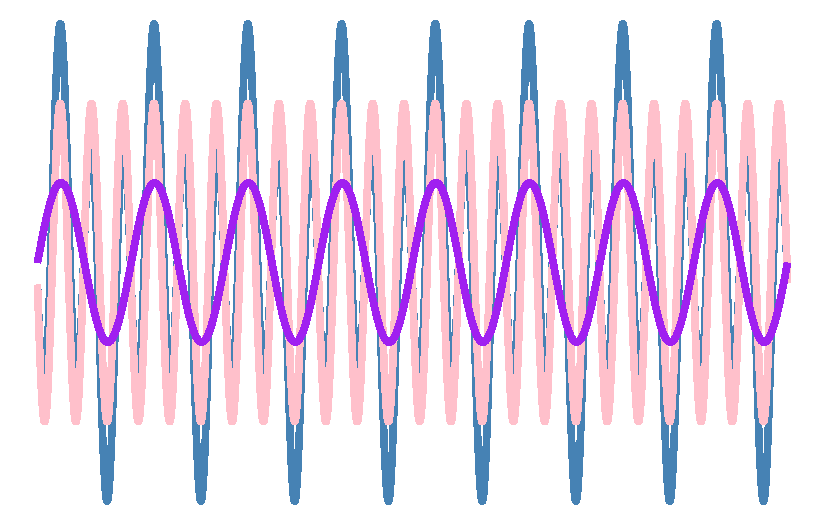
\includegraphics{06-writing-reports_files/figure-pdf/fig-figure-example-1.pdf}

}

\caption{\label{fig-figure-example}This is an example of a Figure with a
caption.}

\end{figure}

We might want to cross-reference a section in our document. This is
easily done by inserting a tag at the section header such as
\texttt{\{\#sec-cross-reference\}}, this tag can be referenced in text
using \texttt{@sec-cross-reference} resulting in
Section~\ref{sec-cross-reference}. The \texttt{sec-} part is the
required prefix for a section.

For additional details on cross-referencing, see the
\href{https://quarto.org/docs/authoring/cross-references.html}{quarto
documentation on cross-referencing}.

Citations are mandatory in academic writing. Be sure to take advantage
of the built in support for citations. When writing in quarto (or
RMarkdown) we can think of a reference as having three parts. The
identifier, the reference and the style. We use the identifier when
authoring. For example, let's cite the R for Data Science book, we do
this by using the following syntax (Wickham and Grolemund 2017). The
syntax requires that we have linked a bibliography to the document. The
bibliography should include the reference, with the same identifier. The
bibliography is a collection of reference entries written in bibtext
format (see below). It must be included in the document meta data field
(YAML field).

\begin{Shaded}
\begin{Highlighting}[numbers=left,,]
\SpecialCharTok{@}\NormalTok{book\{r4ds,}
\NormalTok{  title}\OtherTok{=}\NormalTok{\{R }\ControlFlowTok{for}\NormalTok{ data science\},}
\NormalTok{  author}\OtherTok{=}\NormalTok{\{Wickham, Hadley and \{\textbackslash{}c\{C\}\}etinkaya}\SpecialCharTok{{-}}\NormalTok{Rundel, Mine and Grolemund, Garrett\},}
\NormalTok{  year}\OtherTok{=}\NormalTok{\{}\DecValTok{2023}\NormalTok{\},}
\NormalTok{  publisher}\OtherTok{=}\NormalTok{\{}\StringTok{" O\textquotesingle{}Reilly Media, Inc."}\NormalTok{\}}
\NormalTok{\}}
\end{Highlighting}
\end{Shaded}

Notice the identifier. When adding the citation \texttt{{[}@r4ds{]}} it
will turn out to (Wickham and Grolemund 2017) in the formatted text and
added to the bottom of the document as a full reference. If we want
another \emph{citation style} we can specify a file responsible for
citation styles. The default is the Chicago style. Specifying a citation
style file in YAML will change the style, for example
\texttt{csl:\ my-citation-style.csl} tells quarto to use the file
\texttt{my-citation-style.csl} when formatting citations. This file can
be edited or copied from a large collection of possible styles located
in the \href{https://github.com/citation-style-language/styles}{citation
style language repository}. The repository is hosted on GitHub and
searchable, click ``Go to file'' and type ``vancouver'' to get examples
of CSL files that uses a Vancouver-type citation style.

Footnotes can be handy when writing. In the default mode, these will be
included as superscript numbers, like this\footnote{This is a footnote.},
numbered by order of appearance.

The syntax for including footnotes is straight forward. Notice that the
text for the footnote is included below the paragraph using the
identifier created in the text.

\begin{Shaded}
\begin{Highlighting}[numbers=left,,]
\NormalTok{Footnotes can be handy when writing. In the default mode, }
\NormalTok{these will be included as superscript numbers, like }
\NormalTok{this[}\SpecialCharTok{\^{}}\NormalTok{footnote], numbered by order of appearance. }

\NormalTok{[}\SpecialCharTok{\^{}}\NormalTok{footnote]}\SpecialCharTok{:}\NormalTok{ This is a footnote.}
\end{Highlighting}
\end{Shaded}

See the quarto documentation on
\href{https://quarto.org/docs/authoring/footnotes-and-citations.html}{citations
and footnotes}.

see also \href{https://r4ds.hadley.nz/quarto.html}{Chapter 29 in R for
data science}.

\hypertarget{additional-files-and-folder-structures-in-a-complete-analysis-project}{%
\section{Additional files and folder structures in a complete analysis
project}\label{additional-files-and-folder-structures-in-a-complete-analysis-project}}

As we starting to notice, a report authored in quarto or R Markdown
often requires additional files to render properly. We might have a
collection of references, some data sets and possibly some analysis
files that are not included in the quarto or R markdown file. To keep
everything organized I recommend a general folder structure for every
analysis project. This structure might change as the project grows or
changes. The parts listed below are what I usually end up with as a
common set in the majority of projects I work with\footnote{This
  organization was initially inspired by
  \href{https://kbroman.org/steps2rr/pages/organize.html}{Karl Broman's}
  steps towards reproducible science.}.

\hypertarget{the-readme-file}{%
\subsection{The readme-file}\label{the-readme-file}}

The README-file can be, or should be an important file for you. When a
project is larger than very tiny, it becoms complex and you should
include a README-file to tell others and yourself what the project is
about and how it is organized. Creating a file called \texttt{README.md}
in a GitHub folder automatically renders it on the main page of your
repository (more about that later). Here you have the opportunity to
outline the project and explain the organization of your projects
folder/repository.

I find it very helpful to work with the README-file continuously as the
project evolves. It helps me remember where the project is going.

A very basic ouline of the README-file can be

\begin{Shaded}
\begin{Highlighting}[numbers=left,,]
\CommentTok{\# My project}

\NormalTok{Author}\SpecialCharTok{:} 
\NormalTok{Date}\SpecialCharTok{:} 

\DocumentationTok{\#\# Project description }
\NormalTok{A description of what this prject is about, the }
\NormalTok{purpose and how to get there. }

\DocumentationTok{\#\# Organization of the repository}

\NormalTok{Files are organized as...}

\DocumentationTok{\#\# Changes and logs}
\DecValTok{2023{-}08{-}15}\SpecialCharTok{:}\NormalTok{ Added a description of the project...}
\end{Highlighting}
\end{Shaded}

\hypertarget{resources-2}{%
\subsection{\texorpdfstring{\texttt{/resources}}{/resources}}\label{resources-2}}

I usually include a sub-folder called \texttt{resources}. Here I keep
CSL-files, the bibliography, any styling or templates used to render the
report. Keeping this in a separate folder keeps the top-folder clean.

\hypertarget{data}{%
\subsection{\texorpdfstring{\texttt{/data}}{/data}}\label{data}}

The \texttt{data} folder is an important one. Here I keep all data that
exists as e.g., \texttt{.csv} or \texttt{.xlsx} files. If I create data
in the project, such as combined data sets that are stored for more
convienient use, I keep these in a sub-folder (e.g.,
\texttt{data/derived-data/})\footnote{Again, an important note from
  \href{https://kbroman.org/steps2rr/pages/organize.html}{Karl Broman,
  ``Organize your data and code''}}. If there is a lot of raw
unprocessed data, these might be stored in \texttt{data/raw-data/} with
specific sub-folders.

\hypertarget{figures}{%
\subsection{\texorpdfstring{\texttt{/figures}}{/figures}}\label{figures}}

If you want to make figures for presentations or submission to a
journal, you might want to save output as \texttt{.tiff} or
\texttt{.pdf} files. When doing this it might be a good idea to
structure a figure-folder with e.g.~\texttt{figure1.R} that renders to
e.g.~\texttt{figure1.pdf}. If you only include figure output in the
quarto, the figure folder might contain R-scripts that produces the
figures. The end results are included in the quarto document by sourcing
the R-script. This detour might make it easier to find code for a
specific figure once your project is large enough.

\hypertarget{r}{%
\subsection{\texorpdfstring{\texttt{/R}}{/R}}\label{r}}

R-scripts that are not figures but contains analyses or data cleaning or
the like can be stored in R scripts in a specific folder. The reason to
keep R scripts separate from a quarto file might be that they are large
and produces some output, like a data set, that is later used in the
report file. It makes it easier to find and work on specific code
without breaking other parts of your project. Actually, it is a good
idea to ``build'' the parts of your analysis as smaller parts.

\hypertarget{quarto-formats}{%
\section{Quarto formats}\label{quarto-formats}}

Quarto brings many possibilities for authoring data-driven formats,
including but not restricted to websites, books, blogs and
presentations. In this course

\hypertarget{references-and-footnotes-5}{%
\section{References and footnotes}\label{references-and-footnotes-5}}

\bookmarksetup{startatroot}

\hypertarget{version-control-and-collaboration}{%
\chapter{Version control and
collaboration}\label{version-control-and-collaboration}}

In the previous chapter we underlined the importance of the project as a
way of keeping data, code (and text) in an organized manner. The project
concept in RStudio can easily be extended to include version control.
Version control also makes collaboration easier. Most often,
collaborating on writing a report, assignment or paper is hard. You send
a file, get another one in return. Some files are on dropbox, some are
lost. What if we had a system for collaboration that made it easy to
follow the progress of a project. Connecting RStudio projects to git and
GitHub makes this possible.

\hypertarget{why-version-control}{%
\section{Why version control}\label{why-version-control}}

\href{www.github.com}{Github} is a platform for collaborative coding. As
we have noted before, collaboration concerns both others and you, in the
future! This means that having a formal system for keeping track of your
projects is a good thing.

Github also provides version control. Version control can help you track
changes in your entire analysis or writing project. This is helpful when
multiple files make up a complex project, including e.g.~scripts, data
and manuscript files. It is also helpful when multiple collaborators
work together (e.g.~writing a report). You will, by using version
control, avoid overwriting other peoples work. With multiple changes
made to the project, \textbf{merging} will create the latest up-to-date
version. When you change a file in your analysis you will be required to
describe the changes you have made. Git creates a record of your
changes. This also means that we have ``backups'' of previous versions.

\hypertarget{three-ways-of-hooking-up-to-github}{%
\section{Three ways of hooking up to
GitHub}\label{three-ways-of-hooking-up-to-github}}

\hypertarget{create-a-new-repository-on-github-and-clone-it}{%
\subsection{Create a new repository on GitHub and clone
it}\label{create-a-new-repository-on-github-and-clone-it}}

Access your personal GitHub account and click \textbf{New} under
repositories. This is equivalent to going to \url{www.github.com/new}.
GitHub will ask for a repository name, a description and whether you
want the repository to be public or not. You can also chose to add a
Readme-file.

Names and descriptions are important, a better name and description
makes it easier for you and others to find and make use of your
repository. Even when making repositories for school assignments, a good
name will likely make it more re-usable in the future. The same is true
for the readme file. So, name the repository with a \textbf{descriptive
name}, write a short \textbf{description with the purpose} of the
repository and \textbf{add a readme-file} to the repository.

A public repository is open for everyone, private repositories have
restricted access.

Once the repository is created you can clone it. This means that you
will copy the content to your local machine (PC/Mac). In RStudio this is
most conveniently done by starting a new RStudio project and selecting
\emph{Version Control} in the project menu. You will be asked to copy
the address shown under ``Code'' on GitHub.

\hypertarget{create-an-online-repository-from-a-local-folder}{%
\subsection{Create an online repository from a local
folder}\label{create-an-online-repository-from-a-local-folder}}

Let's say that we have a local folder that is a RStudio Project, without
version control and we want to create a online repository together with
version control. We can use GitHub desktop to accomplish this or GitHub
CLI.

\textbf{Using the terminal and GitHub desktop:}

\begin{enumerate}
\def\labelenumi{\arabic{enumi}.}
\tightlist
\item
  The first step is to make the local folder a git repository, in
  RStudio with the project running go to a terminal and type
  \texttt{git\ init}. The terminal will let you know that you have
  initialized a git repository.
\item
  Start up GitHub desktop, under \emph{File} choose \emph{Add local
  repository} and find the folder on your computer where you have your
  RStudio project. Once open in GitHub desktop you will see all changes
  and additions of new files.
\item
  Commit your changes by writing a first commit message, and possibly a
  longer description of the commit.
\item
  Click ``Publish repository'', you will be asked to edit the name and
  description of the repository and choose whether to have the
  repository private or not (see above for recommendations).
\item
  Go to GitHub.com and check if the repository is published.
\end{enumerate}

\textbf{Using the terminal and GitHub terminal client (CLI):}

\begin{enumerate}
\def\labelenumi{\arabic{enumi}.}
\tightlist
\item
  Be sure to be in your RStudio project and use the terminal in RStudio
  to initiate a git repository, type \texttt{git\ init} in the terminal.
\item
  Also in the terminal type \texttt{gh\ repo\ create}, this will guide
  you through the same process as with GitHub desktop but all selections
  are done in the terminal.
\end{enumerate}

\hypertarget{create-an-online-repository-from-a-local-git-repository}{%
\subsection{Create an online repository from a local git
repository}\label{create-an-online-repository-from-a-local-git-repository}}

If you have already initialized a RStudio project as a git repository
you can follow the steps above without the \texttt{git\ init} command.
Using \texttt{git\ init} on an already initialized git repository will
reinitialize it. This will not remove git history of the repository (see
\href{https://git-scm.com/docs/git-init}{here for documentation}).

\hypertarget{git-commands-and-workflows}{%
\section{Git commands and workflows}\label{git-commands-and-workflows}}

\hypertarget{add-commit-and-push}{%
\subsection{Add, commit and push}\label{add-commit-and-push}}

The day to day workflow when working on a git project involves making
changes to your files and saving those changes locally, and in the
version control system. By the end of the day you might also want to
make sure all changes are synchronized with the online repository.

This workflow includes the git commands \texttt{add}, \texttt{commit}
and \texttt{push}.

Using the terminal \texttt{git\ add\ \textless{}filename\textgreater{}}
or \texttt{git\ add\ -A} adds a specific file or all changes to a list
of changes to be ``committed'' into version history. The equivalent
operation in GitHub desktop is checking all boxes under changes. This is
done automatically and you have to uncheck files or changes that you do
not want to commit to history.

In the terminal we can commit changes to the git history using the
command \texttt{git\ commit\ -m\ "a\ commit\ description\ message"} the
additional part \texttt{-m\ "a\ commit...} is the required commit
message. It is good to be informative if you need to find a specific
change to a file. In GitHub desktop this is easily done by writing a
commit message under \emph{summary} in the bottom left corner once you
have changes in your repository.

The last step, \texttt{git\ push}, means that you are uploading all
changes to the online repository. This will update the repository on
GitHub, your version history is now up to date in your online
repository. This also means that you have an online backup of your work.

\hypertarget{collaboration-pull-clone-and-fork}{%
\subsection{\texorpdfstring{Collaboration, \texttt{pull}, \texttt{clone}
and
\texttt{fork}}{Collaboration, pull, clone and fork}}\label{collaboration-pull-clone-and-fork}}

Collaboration is most often done with yourself in the future. The
\texttt{git\ pull} command (using the terminal) downloads all changes to
your working directory. You want to do this when you have changes in the
online repository that is not synchronized with the local repository.
This might be the case if you have made changes to your repository on
GitHub, like added a readme file. Or if you are collaborating with
someone who have made changes to the repository. I work on multiple
computers, sometimes on the same repository, the online repository is
where a keep the most up to date version of my project.

Using GitHub desktop, we can click \emph{Fetch origin} to get the latest
changes from the online repository. GitHub desktop will suggest to pull
these changes to the working directory after you have done this
operation.

We have already covered \texttt{git\ clone}, this essentially means
downloading an online repository to your local machine. This is most
easily done while initializing a new RStudio project.

A fork is a copy of someones online repository that is created as a new
repository under your user. You now have access to this repository and
can make changes. The repository can have its own life or be used to
create changes that later are suggested as changes to the ``parent
repository''.

In this course you can fork a template for the portfolio exam. This is
an example where your fork will have its own life.

If a fork is used to suggest changes this is done through a \emph{pull
request}. Using the web client (GitHub), we can click \emph{create pull
request} when inside a forked repository. This will take you a few steps
where you are expected to describe changes to the repository. The
original author will get a notification to review the pull request and
can chose to incorporate the changes into the parent repository.

\hypertarget{branches}{%
\subsection{Branches}\label{branches}}

Much like a fork, we can create copies of our own repository. These are
called branches. A branch might contain changes that we want to try out
before we make it the ``official'' version of our repository. These
changes can include experiments that might mess up things or break code.

Using GitHub desktop we can create a new branch by clicking
\emph{Current branch} in the upper left and then \emph{Create branch}.

\hypertarget{additional-great-things-about-github}{%
\section{Additional great things about
GitHub}\label{additional-great-things-about-github}}

GitHub has great capabilities for managing projects. You can for
example:

\begin{itemize}
\tightlist
\item
  Post \textbf{issues} that are suggestions or questions regarding a
  repository. Issues can be categorized with labels and assigned.
\item
  You can create to-do lists in the Projects tab (in the web interface).
  This could be a nice way of sharing and tracking the progress of a
  project.
\item
  You can build a wiki. This is simply a collection of pages that can be
  used to document the repository or a project (in a wider sense) that
  you are working on.
\item
  All of the above can be private and public. You can choose whom have
  access to your repository. This makes it easy to work on a project
  even if you need to keep things a secret.
\end{itemize}

In this course I want you to contribute to the wiki pages of the course.
The wiki is hosted at
\href{https://github.com/dhammarstrom/IDR4000-2021}{github.com/dhammarstrom/IDR4000-2021}.
To contribute you need to have created your own GitHub user account.

\hypertarget{when-will-this-knowledge-be-handy}{%
\section{When will this knowledge be
handy?}\label{when-will-this-knowledge-be-handy}}

When writing your master thesis, it will be extremely easy to share your
code with your supervisor or other students, whit whom you collaborate.
You can just invite someone to make changes in your repository and then
download them. As noted several times before, your most frequent
collaborator is you. Using git makes it easy to keep track of changes in
your project and it keeps your most frequent collaborator from messing
up your work.

Version control workflows are part of almost all technology companies,
and will most certainly be part of many more types of businesses,
institutions and workplaces in the future as we need to collaborate on
large, complex projects. Knowing about these systems is in that sense
quite handy!

\hypertarget{resources-3}{%
\section{Resources}\label{resources-3}}

There are of course more functions in git, here are some resources for
deeper understanding.

\begin{itemize}
\tightlist
\item
  \href{https://happygitwithr.com/}{Extensive resources can be found on
  Happy Git and GitHub for the useR}
\item
  \href{https://kbroman.org/github_tutorial/}{Karl Broman provides a
  ``minimal tutorial''}
\item
  \href{https://try.github.io/}{GitHub hosts resources for learning Git}
\end{itemize}

\hypertarget{refs}{}
\begin{CSLReferences}{1}{0}
\leavevmode\vadjust pre{\hypertarget{ref-RN2391}{}}%
Broman, Karl W., and Kara H. Woo. 2018. {``Data Organization in
Spreadsheets.''} Journal Article. \emph{The American Statistician} 72
(1): 2--10. \url{https://doi.org/10.1080/00031305.2017.1375989}.

\leavevmode\vadjust pre{\hypertarget{ref-refID1}{}}%
Ellefsen, S., D. Hammarstrom, T. A. Strand, E. Zacharoff, J. E. Whist,
I. Rauk, H. Nygaard, et al. 2015. {``{Blood flow-restricted strength
training displays high functional and biological efficacy in women: a
within-subject comparison with high-load strength training}.''}
\emph{Am. J. Physiol. Regul. Integr. Comp. Physiol.} 309 (7): R767--779.

\leavevmode\vadjust pre{\hypertarget{ref-RN2358}{}}%
Hammarström, Daniel, Sjur Øfsteng, Lise Koll, Marita Hanestadhaugen,
Ivana Hollan, William Apró, Jon Elling Whist, Eva Blomstrand, Bent R.
Rønnestad, and Stian Ellefsen. 2020. {``Benefits of Higher
Resistance-Training Volume Are Related to Ribosome Biogenesis.''}
Journal Article. \emph{The Journal of Physiology} 598 (3): 543--65.
\url{https://doi.org/10.1113/JP278455}.

\leavevmode\vadjust pre{\hypertarget{ref-RN2225}{}}%
Haun, C. T., C G. Vann, C. Brooks Mobley, Shelby C. Osburn, Petey W.
Mumford, Paul A. Roberson, Matthew A. Romero, et al. 2019.
{``Pre-Training Skeletal Muscle Fiber Size and Predominant Fiber Type
Best Predict Hypertrophic Responses to 6 Weeks of Resistance Training in
Previously Trained Young Men.''} Journal Article. \emph{Frontiers in
Physiology} 10 (297). \url{https://doi.org/10.3389/fphys.2019.00297}.

\leavevmode\vadjust pre{\hypertarget{ref-RN2149}{}}%
Haun, C. T., C. G. Vann, C. B. Mobley, P. A. Roberson, S. C. Osburn, H.
M. Holmes, P. M. Mumford, et al. 2018. {``Effects of Graded Whey
Supplementation During Extreme-Volume Resistance Training.''} Journal
Article. \emph{Front Nutr} 5: 84.
\url{https://doi.org/10.3389/fnut.2018.00084}.

\leavevmode\vadjust pre{\hypertarget{ref-RN1953}{}}%
Ioannidis, John P. A. 2005. {``Why Most Published Research Findings Are
False.''} Journal Article. \emph{PLOS Medicine} 2 (8): e124.
\url{https://doi.org/10.1371/journal.pmed.0020124}.

\leavevmode\vadjust pre{\hypertarget{ref-RN1955}{}}%
Leek, J. T., and R. D. Peng. 2015. {``Statistics: P Values Are Just the
Tip of the Iceberg.''} Journal Article. \emph{Nature} 520 (7549): 612.
\url{https://doi.org/10.1038/520612a}.

\leavevmode\vadjust pre{\hypertarget{ref-RN1492}{}}%
Peng, R. D., F. Dominici, and S. L. Zeger. 2006. {``Reproducible
Epidemiologic Research.''} Journal Article. \emph{Am J Epidemiol} 163
(9): 783--89. \url{https://doi.org/10.1093/aje/kwj093}.

\leavevmode\vadjust pre{\hypertarget{ref-RN2902}{}}%
Spiegelhalter, D. J. 2019. \emph{The Art of Statistics : How to Learn
from Data}. Book. First US edition. New York: Basic Books.

\leavevmode\vadjust pre{\hypertarget{ref-RN2928}{}}%
Stephen, G. Powell, R. Baker Kenneth, and Lawson Barry. 2009. {``Errors
in Operational Spreadsheets.''} Journal Article. \emph{Journal of
Organizational and End User Computing (JOEUC)} 21 (3): 24--36.
\url{https://doi.org/10.4018/joeuc.2009070102}.

\leavevmode\vadjust pre{\hypertarget{ref-RN1956}{}}%
Wickham, Hadley. 2014. {``Tidy Data.''} Journal Article. \emph{Journal
of Statistical Software; Vol 1, Issue 10 (2014)}.
\url{https://www.jstatsoft.org/v059/i10}.

\leavevmode\vadjust pre{\hypertarget{ref-r4ds}{}}%
Wickham, Hadley, and Garrett Grolemund. 2017. \emph{R for Data Science:
Import, Tidy, Transform, Visualize, and Model Data}. 1st ed. Paperback;
O'Reilly Media. \url{http://r4ds.had.co.nz/}.

\leavevmode\vadjust pre{\hypertarget{ref-RN2927}{}}%
Ziemann, Mark, Yotam Eren, and Assam El-Osta. 2016. {``Gene Name Errors
Are Widespread in the Scientific Literature.''} Journal Article.
\emph{Genome Biology} 17 (1): 177.
\url{https://doi.org/10.1186/s13059-016-1044-7}.

\end{CSLReferences}


\backmatter

\end{document}
